\chapter{Background Estimation}\label{chapter:bkg}
%This chapter discusses how the simulation samples considered for the signal and background processes were used to model 
%
%
%describes the event selection criteria used for the signal and control regions used in this search, the blinding method used, and the background processes that were considered.

%Monte Carlo simulated samples are used to model the signal and background processes expected to be observed in the proton-proton collision data used.
%
%
%
%all the effects observed in 
%
%Typically, most of the discrepancies observed can be accounted for by applying various corrective scale factors.
%Where a particular process is poorly described and/or lacking sufficient statistics in the signal region, data-driven estimates of the background are used to model ...

\section{Data and Simulation Samples}\label{sec:samples}
Out of the 37.8\fbinv of  proton-proton collision data at $\sqrt{s} = 13\TeV$ collected by the CMS experiment during 2016, 35.9\fbinv was certified by the collaboration as being of sufficient quality to be used for physics analysis.
The difference between the certified value and the total data recorded is the result of various factors such as the unavailability of a detector due to power failures.
Events are considered from the dataset certified to be good for physics if they pass one of the triggers in accordance with the trigger strategy described in Section~\ref{sec:triggerStrategy}.
Due to the prescaling of all of the electron triggers considered during the start of the most luminous runs (as discussed in Section~\ref{sec:triggerStrategy}) the $ee$ channel uses a reduced dataset corresponding to 35.6\fbinv where none of the triggers considered were prescaled.

The MC samples used to model both the model signal and background processes considered here are listed in table~\ref{tab:mcList}.
For each of the processes considered, the table which includes information on the number of events generated, the cross section used in their generation and the order in perturbative accuracy in QCD to which the generators calculated the processes.
The PS and hadronisation stages for all of the samples was performed using PYTHIA 8.
The CUETP8M2T4 underlying event tune was used by PYTHIA 8 for the \ttbar process simulation samples and the CUETP8M1 underlying event tune for all other simulation samples.
The NNPDF3.0 family of PDF sets~\cite{Ball:2012cx} was used in the generation of all of the samples considered.

\begin{table}[htbp]
\topcaption {
The MC processes and their associated sample sizes, cross sections and generators used. Two generators are considered for the simulation of the Z+jets process; both samples are included in the table.
}
\label{tab:mcList}
  \centering
  \resizebox{\textwidth}{!}{
% This right-aligns numbers in column, but centers them under column title.
 \begin{tabular}{cccc}
   \hline
   \textbf{MC process} & \textbf{Events} & \textbf{Cross section (pb)} & \textbf{Generator (Order)}   \\
   \hline
   tZq  & 14.5M & 0.0758  & MADGRAPH5\_aMC@NLO 2.2.2 (NLO) \\
   \hline
   tHq  & 3.5M & 0.07462  & MADGRAPH5\_aMC@NLO 2.2.2 (LO) \\
   \hline
   tWZ/tWll  & 50K & 0.01104  & MADGRAPH5\_aMC@NLO 2.2.2 (LO) \\
   \hline
   single top tW production (t) & 7M & 35.85 & POWHEG (NLO) \\
   single top tW production ($\overline{\text{t}}$) & 6.9M & 35.85 & POWHEG (NLO) \\
   \hline
   single top s-channel & 2.9M & 10.32 & MADGRAPH5\_aMC@NLO 2.2.2 (NLO) \\
   \hline
   single top t-channel (t) & 67.2M & 136.02 & POWHEG (NLO) \\
   single top t-channel ($\overline{\text{t}}$) & 38.8M & 80.95 & POWHEG (NLO) \\
   \hline
   \ttbar & 77.1M & 831.76 & POWHEG (NLO) \\
   \hline
   \ttbarZ $\rightarrow$ ll$\nu\nu$ & 13.9M & 0.2529   & MADGRAPH5\_aMC@NLO 2.2.2 (NLO) \\
   \ttbarZ $\rightarrow$ qq & 749K & 0.5297   & MADGRAPH5\_aMC@NLO 2.2.2 (NLO) \\
   \hline
   \ttbarW $\rightarrow$ l$\nu$ & 5.3M & 0.2001   & MADGRAPH5\_aMC@NLO 2.2.2 (NLO) \\
   \ttbarW $\rightarrow$ qq & 833K & 0.405  & MADGRAPH5\_aMC@NLO 2.2.2 (NLO) \\
   \hline
   \ttbarH $\rightarrow$ bb & 3.8M & 0.2942 & POWHEG (NLO) \\
           $\rightarrow$ non bb & 4.0M & 0.2123 & POWHEG (NLO) \\
   \hline
   W+jets & 24.1M & 61526.7 & aMC@NLO (NLO) \\
   \hline
   Z+jets ($m_{Z} \geq 50\GeVcc $) & 146M & 5765.4 & MADGRAPH5\_aMC@NLO 2.2.2 (LO) \\
   Z+jets ($10 \GeVcc \leq m_{Z} < 50\GeVcc$) & 35.3M & 18610.0 & MADGRAPH5\_aMC@NLO 2.2.2 (LO) \\
   \hline
   Z+jets ($m_{Z} \geq 50\GeVcc $) & 151M & 5765.4 & MADGRAPH5\_aMC@NLO 2.2.2 (NLO) \\
   Z+jets ($10 \GeVcc \leq m_{Z} < 50\GeVcc$) & 106M & 18610.0 & MADGRAPH5\_aMC@NLO 2.2.2 (NLO) \\
   \hline
   WW $\rightarrow$ l$\nu$qq & 9.0M & 49.997  & POWHEG (NLO) \\
      $\rightarrow$ ll$nu\nu$ & 2.0M & 12.178 & POWHEG (NLO) \\
   \hline
   WZ $\rightarrow$ l$\nu$qq & 24.2M & 10.73 & MADGRAPH5\_aMC@NLO 2.2.2 (NLO) \\
      $\rightarrow$ llqq & 26.5M & 5.606 & MADGRAPH5\_aMC@NLO 2.2.2 (NLO) \\
      $\rightarrow$ lll$\nu$ & 1.9M & 5.26 & MADGRAPH5\_aMC@NLO 2.2.2 (NLO) \\
   \hline
   ZZ $\rightarrow$ ll$\nu\nu$ & 8.8M & 0.5644 & POWHEG (NLO) \\
      $\rightarrow$ llqq & 15.3M & 3.222 & MADGRAPH5\_aMC@NLO 2.2.2 (NLO) \\
      $\rightarrow$ llll & 10.7M & 1.204 & MADGRAPH5\_aMC@NLO 2.2.2 (NLO) \\
   \hline
   WWW & 240K & 0.2086 & MADGRAPH5\_aMC@NLO 2.2.2 (NLO) \\
   \hline
   WWZ & 250K & 0.1651 & MADGRAPH5\_aMC@NLO 2.2.2 (NLO) \\
   \hline
   WZZ & 247K & 0.05565 & MADGRAPH5\_aMC@NLO 2.2.2 (NLO) \\
   \hline
   ZZZ & 249K & 0.01398 & MADGRAPH5\_aMC@NLO 2.2.2 (NLO) \\
   \hline
   
 \end{tabular}}
\end{table}

To determine the impact of a variety of different theoretical uncertainties for several of the processes defined in table~\ref{tab:mcList}, dedicated MC samples were used, which are listed in table~\ref{tab:theorySampleList}.
The entries labelled ``scale'', ``matching'', ``isr'' and ``fsr'' correspond to the variations of the theoretical uncertainties considered in this analysis.
These theoretical uncertainties are discussed further in Section~\ref{sec:theorySysts}.

\begin{table}[htbp]
\topcaption {
The dedicated MC samples used to estimate some theoretical uncertainties. The table includes the associated size of the samples, cross sections and generators used.
}
\label{tab:theorySampleList}
  \centering
% \resizebox{\textwidth}{!}{
 \begin{tabular}{cccc}
   \hline
   \textbf{MC process} & \textbf{Events} & \textbf{Cross section (pb)} & \textbf{Generator (Order)}   \\
   \hline
   tZq scale up & 6.9M & 0.0758  & aMC@NLO (NLO) \\
   tZq scale down & 7.0M & 0.0758  & aMC@NLO (NLO) \\
   \hline
   t tW-channel scale up & 998K & 35.85 & POWHEG V2(NLO) \\
   t tW-channel scale down & 994K & 35.85 & POWHEG V2 (NLO) \\
   $\overline{\text{t}}$ tW-channel scale down & 1.0M & 35.85 & POWHEG V2 (NLO) \\
   $\overline{\text{t}}$ tW-channel scale down & 999K & 35.85 & POWHEG V2 (NLO) \\
   \hline
   t t-channel scale up & 5.7M & 136.02 & POWHEG V2 (NLO) \\
   t t-channel scale down & 5.9M & 136.02 & POWHEG V2 (NLO) \\
   t t-channel matching up & 6.0M & 136.02 & POWHEG V2 (NLO) \\
   t t-channel matching down & 6.0M & 136.02 & POWHEG V2 (NLO) \\
   $\overline{\text{t}}$ t-channel scale up & 4.0M & 80.95 & POWHEG V2 (NLO) \\
   $\overline{\text{t}}$ t-channel scale down & 3.9M & 80.95 & POWHEG V2 (NLO) \\
   $\overline{\text{t}}$ t-channel matching up & 4.0M & 80.95 & POWHEG V2 (NLO) \\
   $\overline{\text{t}}$ t-channel matching down & 4.0M & 80.95 & POWHEG V2 (NLO) \\
   \hline
   \ttbar ISR up & 156.5M & 831.76 & POWHEG V2 (NLO) \\
   \ttbar ISR down & 149.8M & 831.76 & POWHEG V2 (NLO) \\
   \ttbar FSR up & 152.6M & 831.76 & POWHEG V2 (NLO) \\
   \ttbar FSR down & 156.0M & 831.76 & POWHEG V2 (NLO) \\
   \ttbar matching up & 58.9M & 831.76 & POWHEG V2 (NLO) \\
   \ttbar matching down & 58.2M & 831.76 & POWHEG V2 (NLO) \\
   \hline   
 \end{tabular}%}
\end{table}

%%% Alt Z+jets 
%During the study of the poor agreement between simulation and data for the aMC@NLO Z+jets samples considered, a number of alternative 
%To determine the impact of a number of theoretical uncertainties for a number of processes, a several dedicated samples, listed in table~\ref{tab:zPlusSamples}, were used.
%These systematic uncertainties are discussed further Section~\ref{sec:subsec:zPlusJetsEstimation}.
%
%\begin{table}[htbp]
%\topcaption {
%The dedicated MC samples used to determine the impact of theoretical uncertainties, including the associated total number of events, cross sections and generators (and order in perturbative QCD accuracy they are calculated to), considered for the search for tZq in the dilepton final state.
%}
%\label{tab:zPlusSamples}
%  \centering
% \resizebox{\textwidth}{!}{
% \begin{tabular}{cccc}
%   \hline
%   \textbf{MC process} & \textbf{Events} & \textbf{Cross section (pb)} & \textbf{Generator (Order)}   \\
%   \hline
%   tZq scale up & 6.9M & 0.0758  & aMC@NLO (NLO) \\
%   \hline   
% \end{tabular}}
%\end{table}
%

\section{Simulation Corrections}\label{sec:simCorrections}
Simulation is unable to fully recreate all the effects observed in data corrective scale factors are used to reweight MC samples on a per event basis to account for possible discrepancies.

These scale factors are used to correct the simulation for any discrepencies in the lepton identification, isolation and reconstruction efficiencies, lepton and jet energy scales and resolutions, b-tagging efficiencies, the poor modelling of pileup in simulation, and the detector resolutions observed in data.

\subsection{Miscalibrated Tracker APV}\label{subsec:hipEffect}
During the first half of data taking in 2016 the silicon strip detector suffered from an instantaneous-luminosity-dependent hit finding inefficiency, which particularly affected high occupancy regions, due to saturation in the pre-amplifier in the front-end electronics~\cite{Fiori:2016ebh}.
This issue was resolved by changing the configuration of the electronics.
The 55\% of the total dataset affected by this issue has since been reprocessed by CMS to mitigate the impact on the quality of the data taken.

Despite this however, there is still a negative impact on the reconstructing tracks efficiency for physics objects that rely upon tracking data.

This reduced detector efficiency is accounted for by using the weighted average of the scale factors that have been derived separately for both the affected and unaffected portions of the dataset.

\subsection{Lepton Efficiency}\label{subsec:leptonRecoSFs}
The identification, isolation and reconstruction efficiency scale factors for leptons are produced centrally by CMS and are determined by using a large sample of of $Z \rightarrow l^{+} l ^{-}$ events and the so-called \emph{tag-and-probe} method~\cite{CMS:2008rxa}.
From a high-purity sub-sample of these events, where the dilepton invariant mass lies within the window $60 < m_{ll} < 120 \GeV$, the lepton that passes a tight selection criteria is ``tagged'' and other lepton is ``probed'' against a loose selection criteria.
For each type and lepton flavour, the efficiency is the fraction of events where the probe leptons passed the selection criteria under study.
The corrective scale factors determined from these efficiencies are used to reweight events as functions of their leptons' \pt, $\eta$, and flavour.

The efficiencies of the triggers used in the analysis were determined using the \emph{cross-trigger} method used in the measurement of the \ttbar production cross section using the $e\mu$ final state by the CMS collaboration~\cite{Khachatryan:2016kzg}.
The implementation of this methodology was validated by reproducing the \ttbar analysis's trigger efficiencies and their statistical uncertainties.

The cross-trigger methodology determines the trigger efficiencies by using events that pass other trigger combinations that are weakly correlated with those used in the analysis, known as \emph{cross-triggers} (X triggers).
The trigger efficiency is estimated as follows:

\begin{equation}
\epsilon_{trigger} = \frac{N_{X triggers + lepton triggers}}{N_{X triggers}} \;
\end{equation}

where $N_{X trigger}$ is the number of events that have passed the analysis' lepton selection criteria and the cross-triggers, and $N_{X triggers + lepton triggers}$ is $N_{X trigger}$ and the number of events that additionally passed at least one of the lepton triggers for the relevant lepton flavour.

As the trigger requirements are applied to both simulated and data events, a scale factor of the ratio of the trigger efficiency in data and in simulation is calculations and used to weight the simulation.
For both the $ee$ and $\mu\mu$ channels in the signal region and the $e \mu$ channel for the \ttbar control region, a constant scale factor was found to be sufficient to account for the differences between data and simulation.

The efficiencies were determined using data and simulated \ttbar events.
The resultant trigger efficiency scale factors applied to simulation are given in table~\ref{tab:triggerSFs} with their associated statistical uncertainties.
The associated systematic uncertainties are discussed in Section~\ref{sec:systematics}.

\begin{table}[htbp]
\topcaption {The trigger efficiencies for the lepton selection criteria for data and simulation and the resultant corrective scale factors applied to simulation. The uncertainties given only include the statistical uncertainty associated with each value. The determination of the systematic uncertainties is given in Section~\ref{sec:systematics}.}
\label{tab:triggerSFs}
  \centering
%  \resizebox{\textwidth}{!}{
 \begin{tabular}{lccc}
   \hline
   \textbf{Channel} & \textbf{$\epsilon _{data}$} & \textbf{$\epsilon _{MC}$} & \textbf{Scale Factor}\\
   \hline   
   $ee$ & 0.976 $\pm$ 0.001 & 0.988 $\pm$ 0.001 & 0.987 $\pm$ 0.001\\
   $\mu\mu$ & 0.985 $\pm$ 0.001 & 0.992 $\pm$ 0.001 & 0.993 $\pm$ 0.000  \\
   $e \mu$ & 0.875 $\pm$ 0.014 & 0.882 $\pm$ 0.019 & 0.991 $\pm$ 0.007\\
   \hline
 \end{tabular}%}
\end{table}

% part 1 mumu
%% data eff 0.98069  +/- -0.00070/0.00073
%% SF 0.98868 +/- 0.00013
%% part 2 mumu
%% data eff 0.99061 +/- -0.00057/0.00061
%% MC 0.99192 +/- -0.00061/0.00074
%% SF 0.99868 +/- 0.00017

%%  lumiRunsBCDEF_{19713.888}, // Lumi for hip era runs
%  lumiRunsGH_{16146.178}, // Lumi for post-hip era runs

\subsection{Lepton Energy Corrections}\label{subsec:leptonEnergyCorrections}
\subsubsection{Electron Regression and Energy Scale and Smearing Corrections}
Energy regression and energy scale and smearing corrections that have been produced by the CMS Electron Gamma (EGM) Physics Object Group are applied to the reconstructed electrons.
The energy regression uses detector information to correct the electron energy recorded in order to obtain the best possible resolution of the reconstructed particle.
The energy scale and smearing corrections are used to correct the energy scale and resolution in simulation.

\subsubsection{Rochester Corrections}
The muon momentum scale and resolution correction methods developed by the University of Rochester~\cite{rochester}, known as \emph{Rochester Corrections}, are used to remove any muon momentum bias arising from any possible detector misalignment and any error in the measurement of the magnetic field for both MC and data.
These corrections are derived using a sample of high \pt $> 20\GeVc$ muons from Z $ \rightarrow \mu^{+}\mu^{-}$ decays using a two-step method.
The first of the two steps determines a correction factor that is defined as the difference in the mean inverse transverse momenta of the muons from a perfectly aligned simulation and reconstructed data or simulation.
These corrections are tuned in the second step using the $M_{\mu^mu}$ peak for a perfectly aligned detector to calibrate the corrections.
This removes any dependence on detector efficiency or physics modelling.

The Rochester Corrections are applied to each muon as an event weight that is a function of the muon's charge, \pt, $\eta$ and $\phi$.

\subsection{Jet Energy Corrections}\label{subsec:jesjer}
As described in Section~\ref{subsubsec:JECs}, the Jet Energy Corrections are applied to account for the non-uniform response in \pT and $\eta$ of the detector by comparing the differences between the generator level and detector level responses in simulation and any residual differences between simulation and data.

In addition to these corrections, as the Jet Energy Resolution (JER) observed in data is approximately 10\% poorer than that observed in simulation, the 4-vectors of simulated jets are smeared as functions of generator level and reconstructed \pt and $\eta$ to account for this~\cite{Khachatryan:2016kdb}.

\subsection{b-tagging Efficiency}\label{subsec:btagEff}
The CMS B-Tag and Vertexing (BTV) Physics Object Group measures the b-tagging efficiency and misidentification rates for b- and light-flavoured jets in data and MC simulation considering both multijet and \ttbar processes for the algorithms that they support~\cite{Sirunyan:2017ezt}.
From these measurements b-tagging efficiency scale factors are produced and provided for analysts to apply to simulated events to correct for differences observed between data and simulation.
These scale factors, as functions of the jet flavour, \pT and $\eta$, are used to alter the weight of the MC events.
This methodology was chosen as it involves only changing the weight of the selected MC events which, unlike other methods, avoids events migrating into different b-tag multiplicity bins and having events with potentially undefined variables such as the top mass.

\subsection{\PU Modelling}\label{subsec:puSF}
It is challenging to model variations in the number of \PU interactions that result from the changing LHC conditions.
To achieve this, MC events are reweighted as a function of the number of primary vertices so that the simulated PU distributions resemble those observed in data.

The \PU SF is determined as a function of the number of primary vertices, $n_{PV}$, by comparing the $n_{PV}$ distribution in minimum bias data over the running period considered to the corresponding $n_{PV}$ distribution in simulated events.

\subsection{Top quark \pt}
A scale factor is used to reweight all simulated \ttbar events to account for the differences in the top quark \pt distribution observed between data and both LO and NLO simulation~\cite{Khachatryan:2015oqa}.

\section{Signal Region Background Estimation}\label{sec:simBackgrounds}

Good agreement between simulation and data is observed in the signal region at each stage of applying selection criteria and simulation corrections, as shown in Figure~\ref{fig:SR_cutFlow}.
The final event yields for each process considered for the $ee$ and $\mu\mu$ channels and their combination is given in table~\ref{tab:signalYields}.

\begin{figure}[h]
\centering
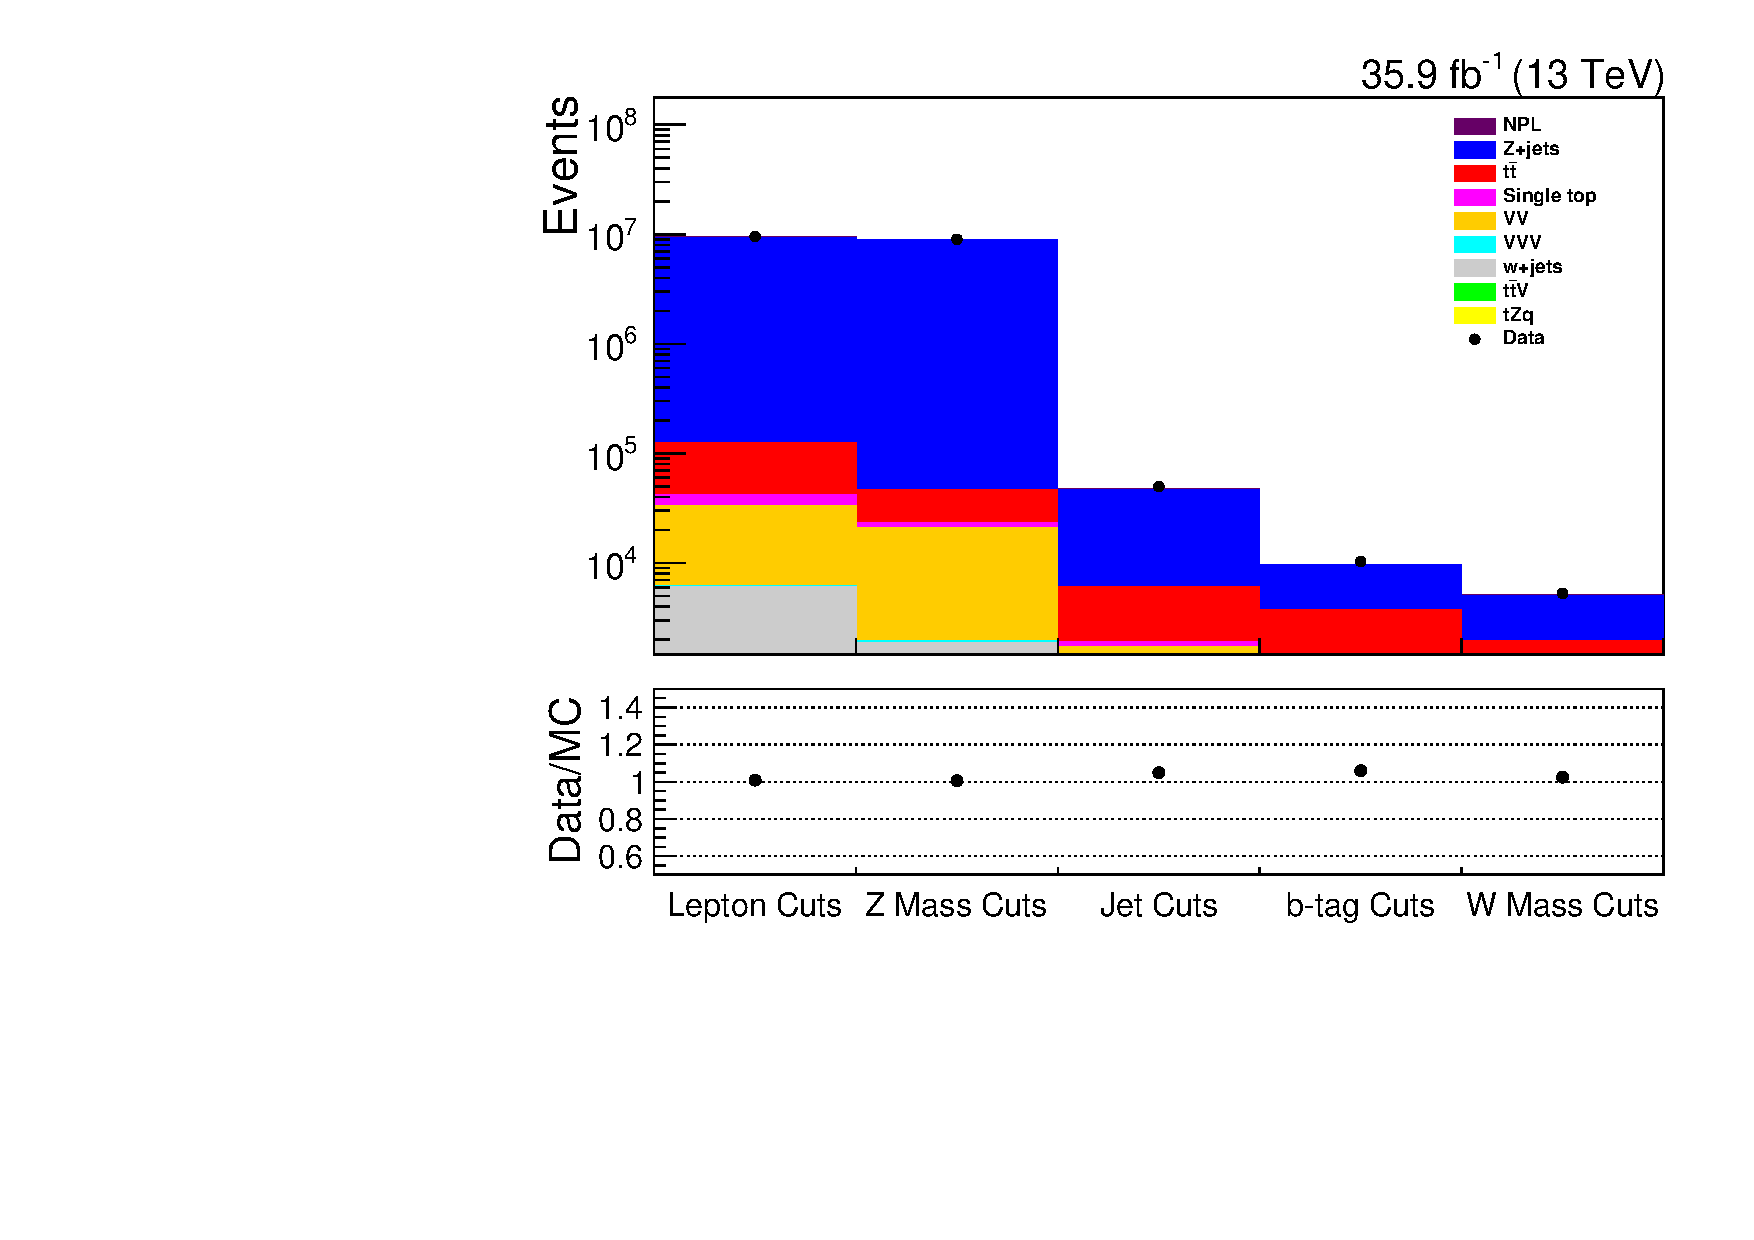
\includegraphics[width=0.47\textwidth]{figs/background-estimation/plots/unblinded/prompt_ee_ttbarInc/cutFlow_log.pdf}
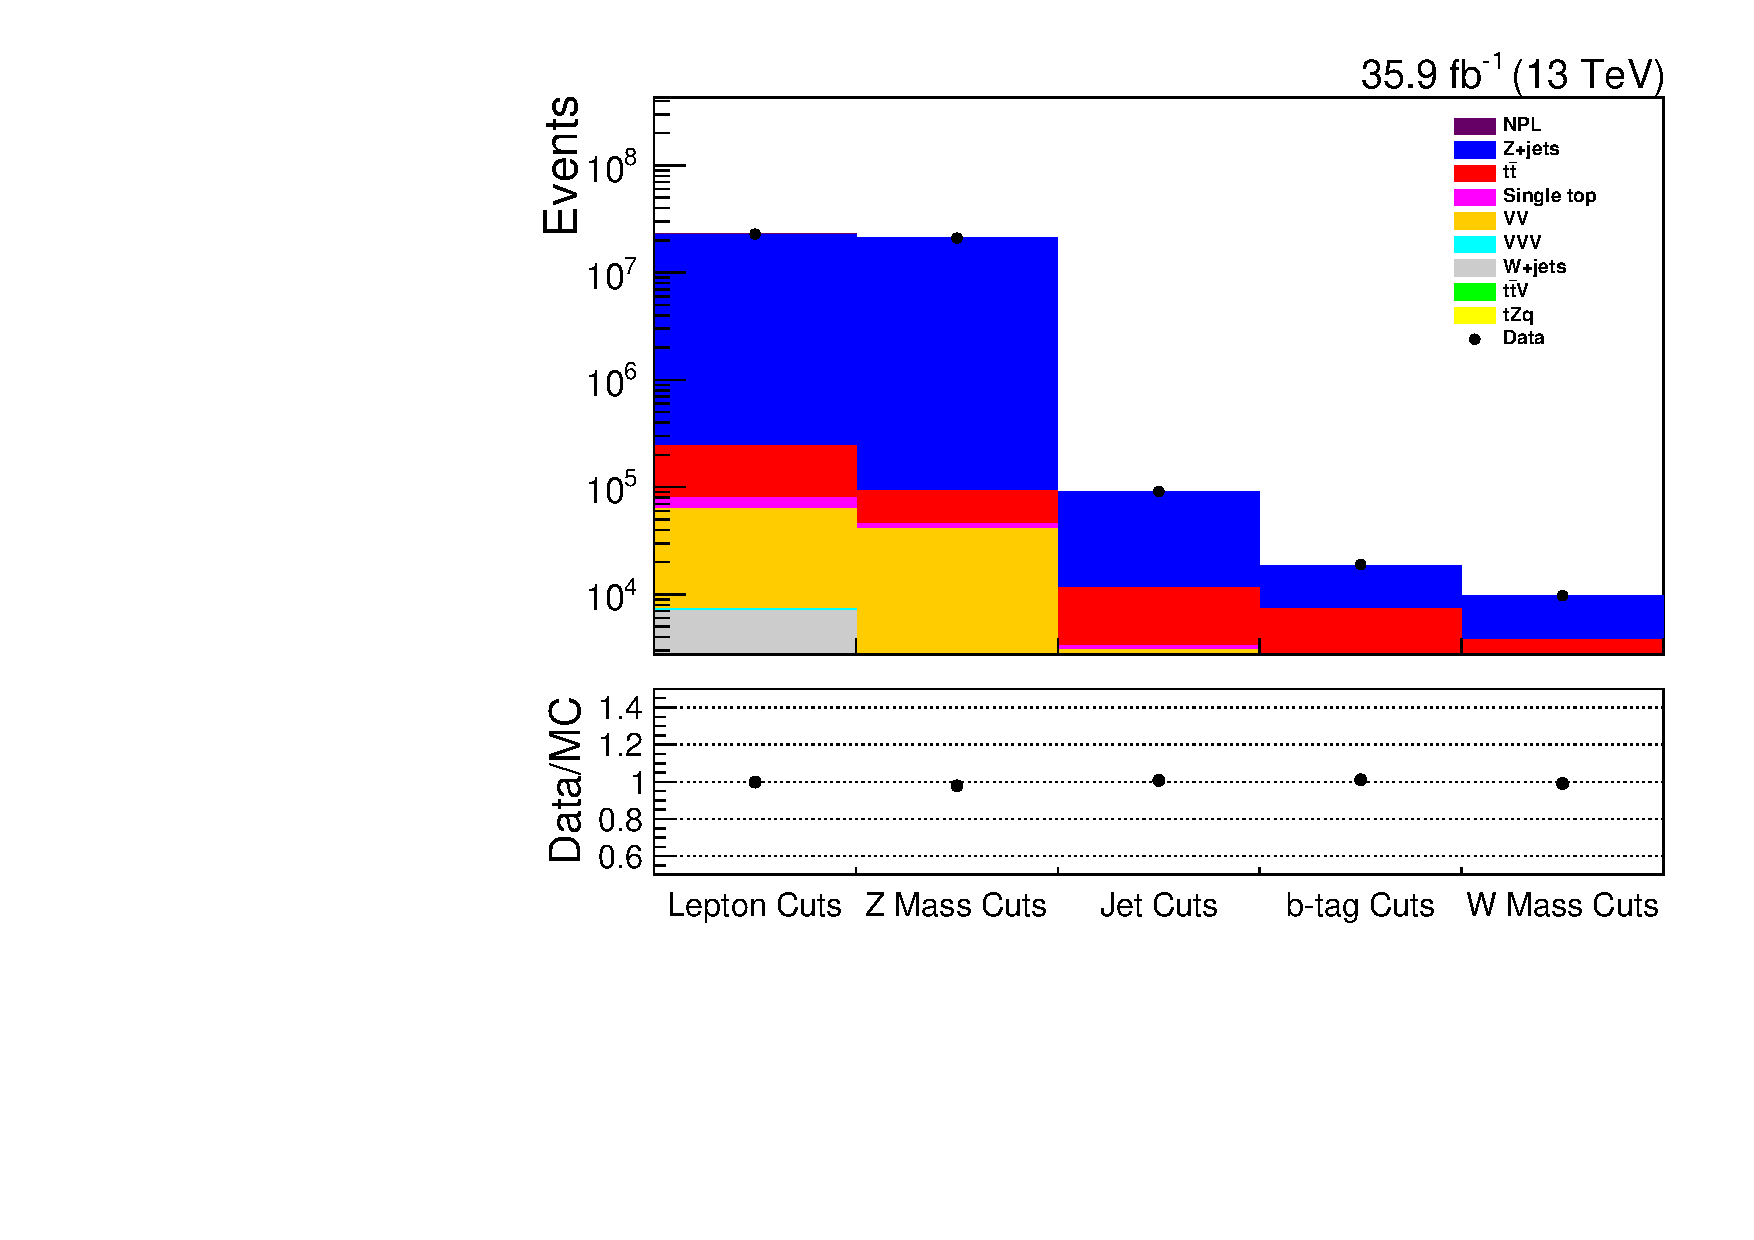
\includegraphics[width=0.47\textwidth]{figs/background-estimation/plots/unblinded/prompt_mumu_ttbarInc/cutFlow_log.pdf}
\caption{
The overall event yield for data and simulation at each stage of applying the signal region selection criteria and simulation corrections for the $ee$ channel (left) and the $\mu\mu$ channel (right).
}
\label{fig:SR_cutFlow}
\end{figure}

\begin{table}[Hp]
\topcaption{The number of observed events in data, expected events in simulation and data and the data-driven estimate of the non-prompt leptons in the signal region following the full event selection. The number of observed events is given for each of the separate channels and their  combination. The statistical uncertainties for each process is given and the LO Z+jets sample is used for the Z+jets contribution.
}\label{tab:signalYields}
\centering
\begin{tabular}{lccc}
\hline
Channel &  $ee$ & $\mu\mu$ & Combined \\
\hline
Signal (SM tZq) & 30.38$\pm$0.07 & 55.49 $\pm$ 0.10 & 85.87 $\pm$ 0.12 \\
Backgrounds: & & & \\
tWZ\@: & 6.44$\pm$0.21 & 10.96$\pm$0.29 & 17.40$\pm$0.36    \\
tHq: & 0.17$\pm$0.01 & 0.37$\pm$0.02 & 0.54$\pm$0.02    \\
ttW\@: & 7.38$\pm$0.14 & 10.83$\pm$0.15 & 18.21$\pm$0.21    \\
ttZ\@: & 62.23$\pm$0.21 & 111.98$\pm$0.29 & 174.21$\pm$0.36    \\
ttH\@: & 4.94$\pm$0.10 & 9.73$\pm$0.14 & 14.67$\pm$0.17    \\
\ttbar: & 1658.73$\pm$23.77 & 3277.48$\pm$34.22 & 4936.21$\pm$41.67    \\
tW\@: & 55.98$\pm$3.02 & 109.59$\pm$4.33 & 165.57$\pm$5.28    \\
s-channel: & 0.0 $\pm$ 0.0 & 0.19$\pm$0.19 & 0.19$\pm$0.19    \\
t-channel: & 0.61$\pm$0.19 & 1.12$\pm$0.25 & 1.73$\pm$0.31    \\
WW\@: & 1.34$\pm$0.47 & 2.29$\pm$0.69 & 3.63$\pm$0.83    \\
WZ\@: & 72.88$\pm$0.67 & 127.32$\pm$0.89 & 200.20$\pm$1.11    \\
ZZ\@: & 51.80$\pm$0.50 & 94.64$\pm$0.68 & 146.44$\pm$0.84    \\
WWW\@: & 0.11$\pm$0.06 & 0.27$\pm$0.10 & 0.38$\pm$0.12    \\
WWZ\@: & 1.32$\pm$0.17 & 2.20$\pm$0.22 & 3.32$\pm$0.28    \\
WZZ\@: & 1.53$\pm$0.11 & 2.62$\pm$0.14 & 4.15$\pm$0.18   \\
ZZZ\@: & 0.65$\pm$0.04 & 1.12$\pm$0.05 & 1.77$\pm$0.06    \\
W+jets: & 0.0$\pm$0.0 & 0.0$\pm$0.0 & 0.0$\pm$0.0    \\
Z+jets: & 3280.20$\pm$62.63 & 5877.51$\pm$87.79 & 9157.71$\pm$107.84    \\
\hline
NPLs: & 69.47$\pm$0.76 & 114.01$\pm$1.25 & 183.48$\pm$2.01   \\
\hline
Total MC & 5236.69$\pm$67.07 & 9695.71$\pm$94.33 & 14932.40$\pm$115.74    \\
Total MC + NPLs & 5306.16$\pm$67.07 & 9754.23$\pm$94.34 & 15060.39$\pm$115.75    \\
\hline
Data & 5274.0$\pm$72.62 & 9750.0$\pm$98.74 & 15024.0$\pm$122.57    \\
\hline
\end{tabular}
\end{table}

In Figure~\ref{fig:SR_cutFlow} it can be seen that the jet cleaning and tight isolation criteria for leptons has significantly reduced the non-prompt lepton contributions, completely removing the W+jets process.
The remaining backgrounds in the signal region consist of processes that involve the decay of a  real Z boson into two leptons or the leptonic decay of two W bosons where the resultant two leptons are consistent with a Z boson decay.
The two dominant background processes are Z+jets and \ttbar, with the single top tW-channel, \ttbarZ, WZ and ZZ processes contributing a similar order of events as tZq processes.
The remaining single top (tHq, tWZ, s-channel, t-channel), \ttbarW, \ttbarH, WW and triboson backgrounds produce contributions smaller than the signal process.

Good agreement between simulation and data is also observed for the reconstructed variables.
Examples of such good agreement include the distributions of the reconstructed Z boson mass following the lepton selection cuts in Figure~\ref{fig:SR_zBoson}; the invariant \pT of all the jets in an event following the jet selection criteria in Figure~\ref{fig:SR_totJetPt}; and the reconstructed W boson following application of the b-tagging criteria in Figure~\ref{fig:SR_wBoson}.

\begin{figure}[h]
\centering
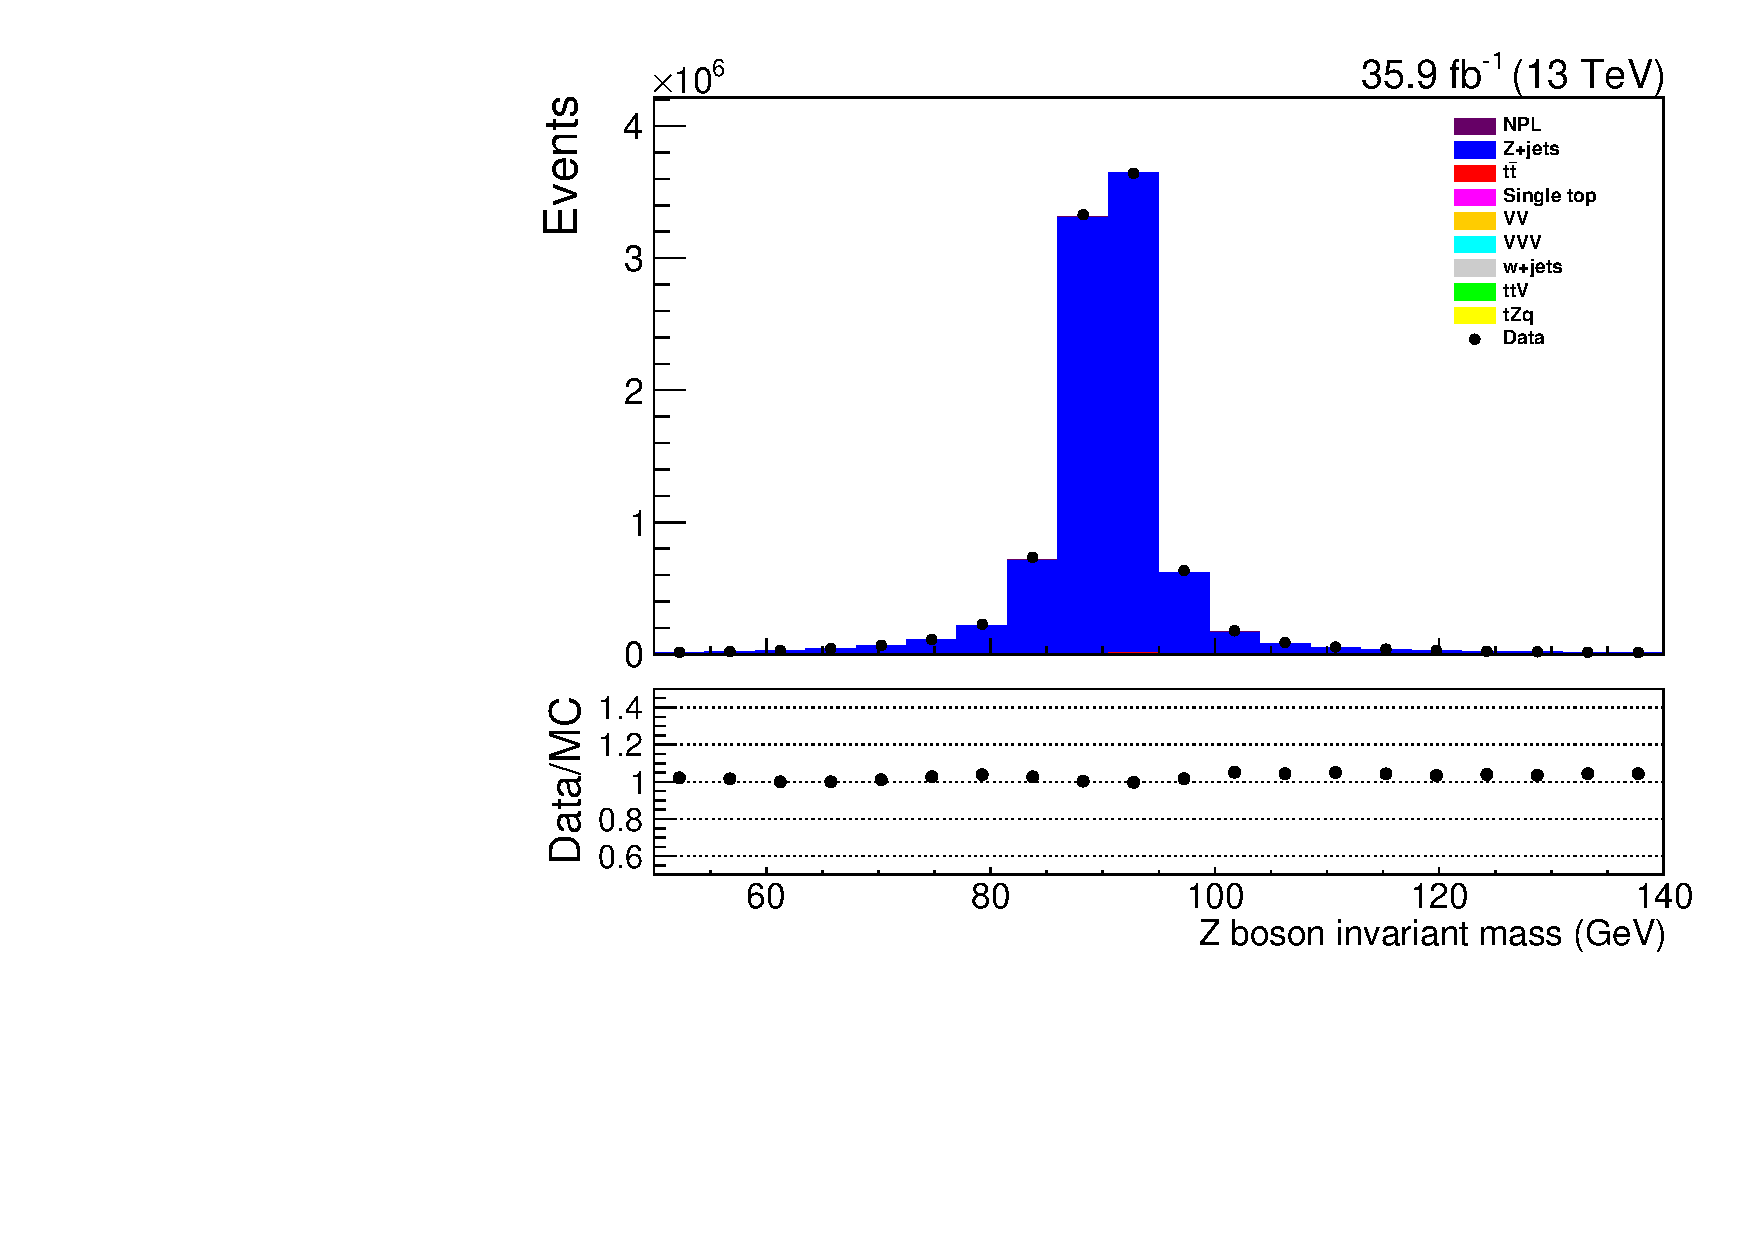
\includegraphics[width=0.47\textwidth]{figs/background-estimation/plots/unblinded/prompt_ee_ttbarInc/zPairMass_NPL_ee_lepSel_ee.pdf}
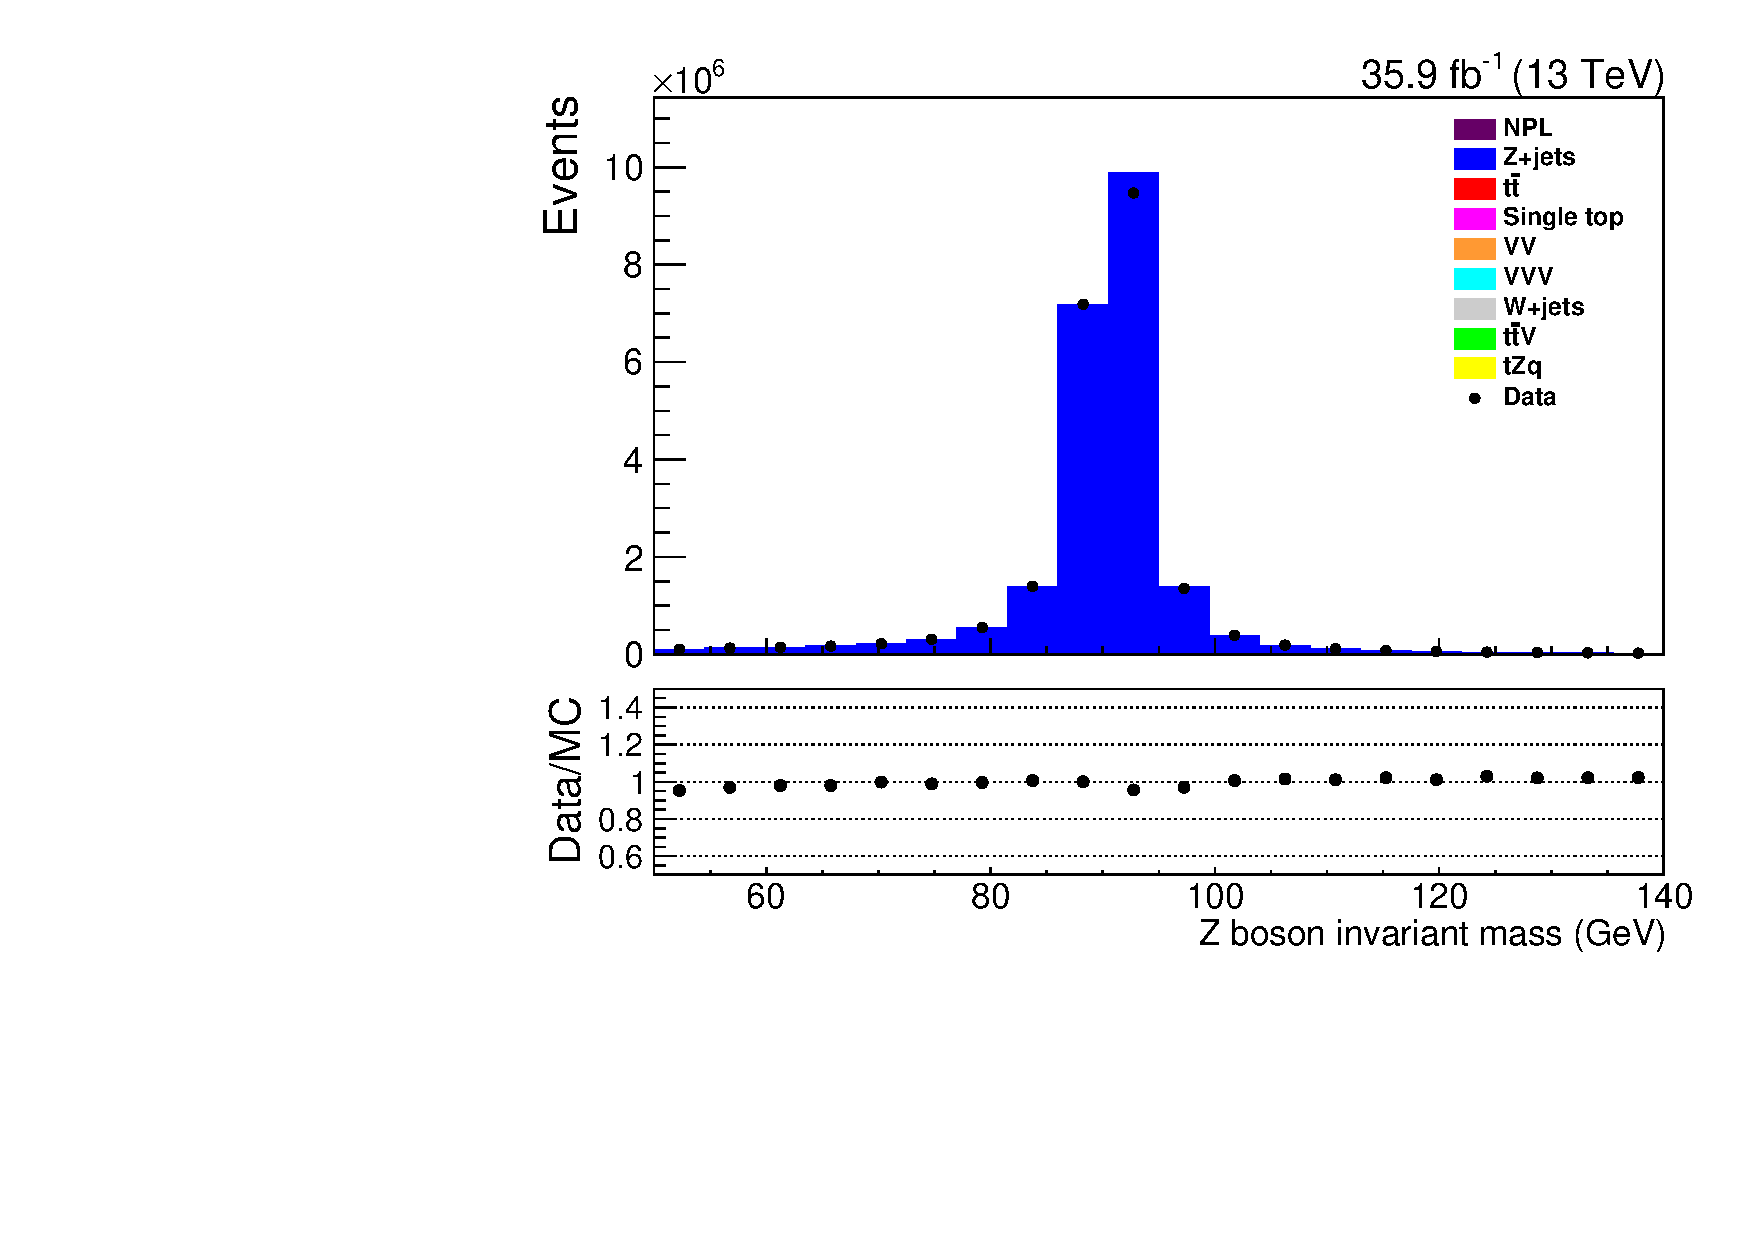
\includegraphics[width=0.47\textwidth]{figs/background-estimation/plots/unblinded/prompt_mumu_ttbarInc/zPairMass_NPL_mumu_lepSel_mumu.pdf}
\caption{
The distributions of the reconstructed Z boson mass for the $ee$ and $\mu\mu$ channels, left and right respectively, following the application of only the lepton selection criteria and corrections.
}
\label{fig:SR_zBoson}
\end{figure}

\begin{figure}[h]
\centering
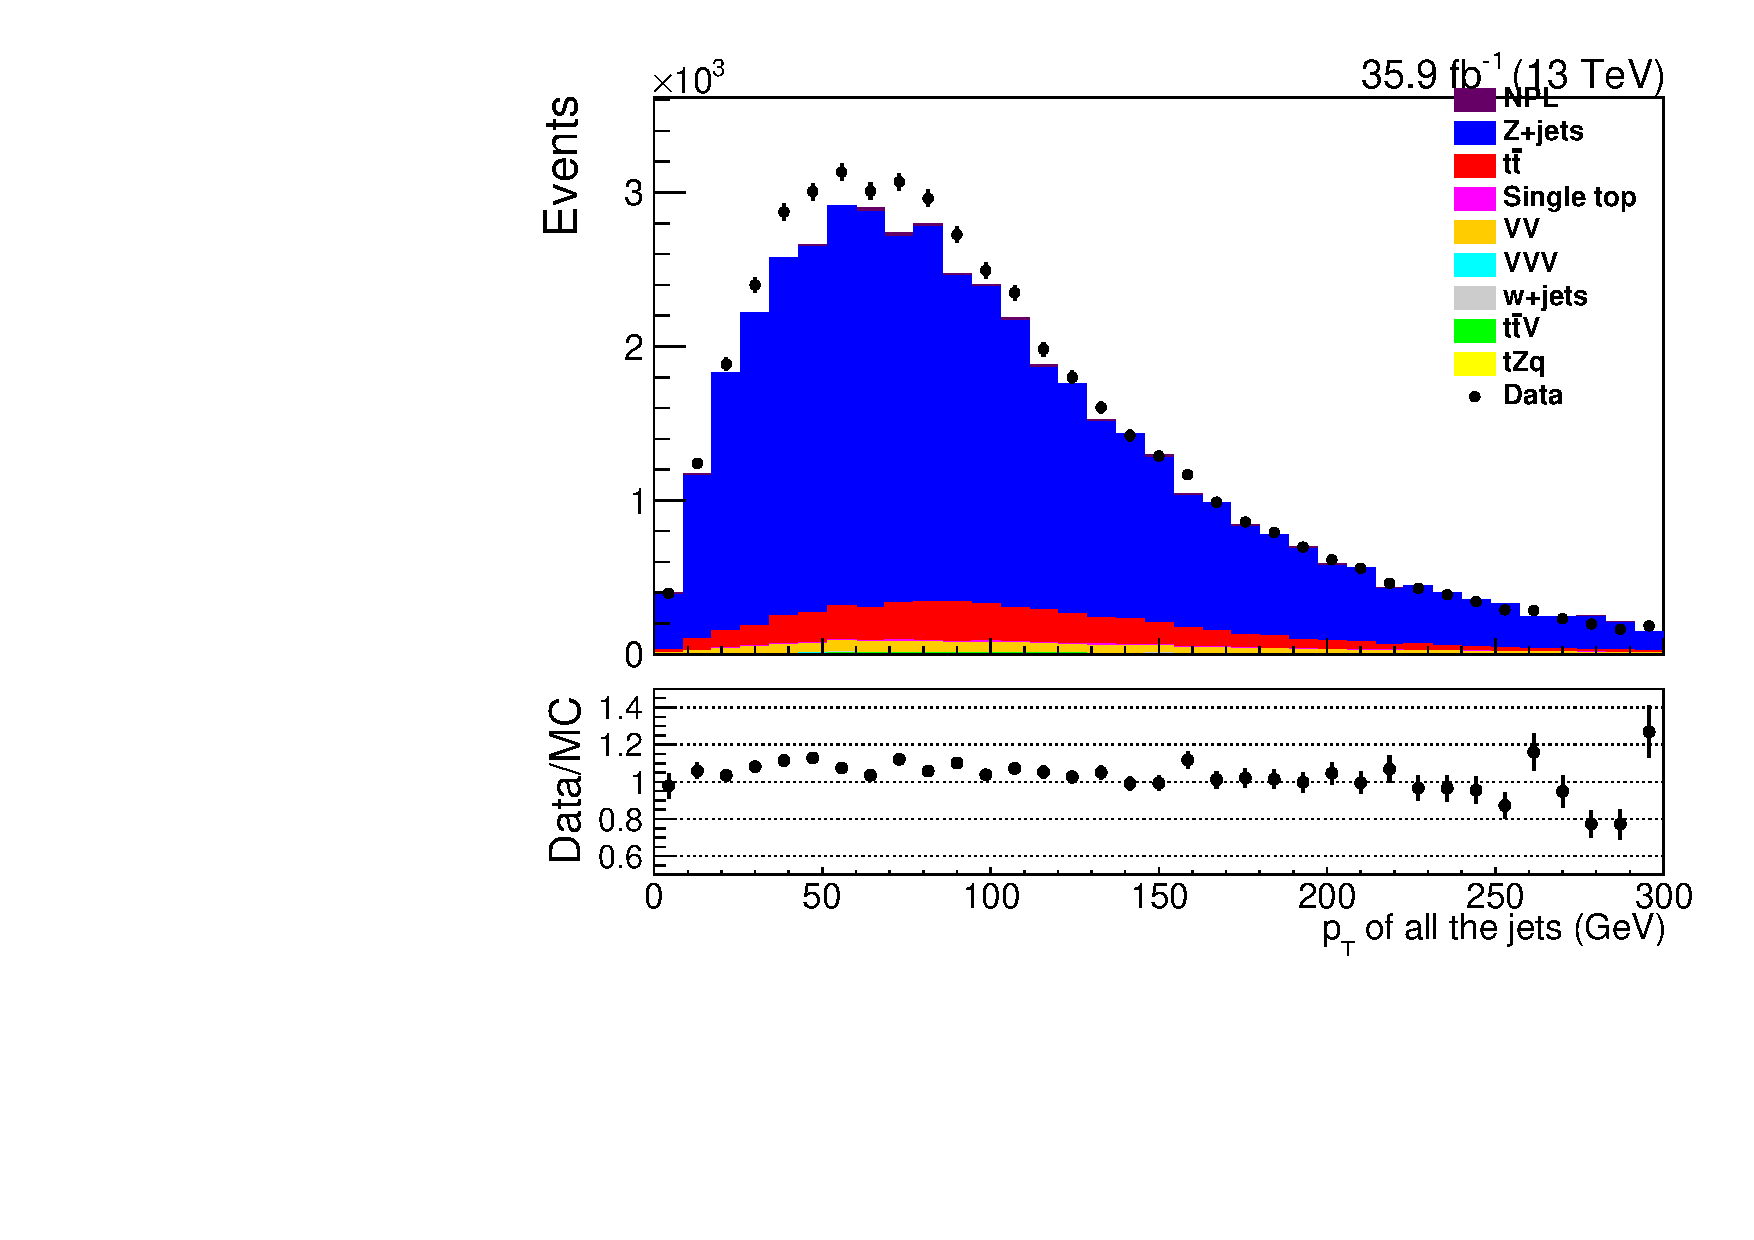
\includegraphics[width=0.47\textwidth]{figs/background-estimation/plots/unblinded/prompt_ee_ttbarInc/totalJetPt_NPL_ee_jetSel_ee.pdf}
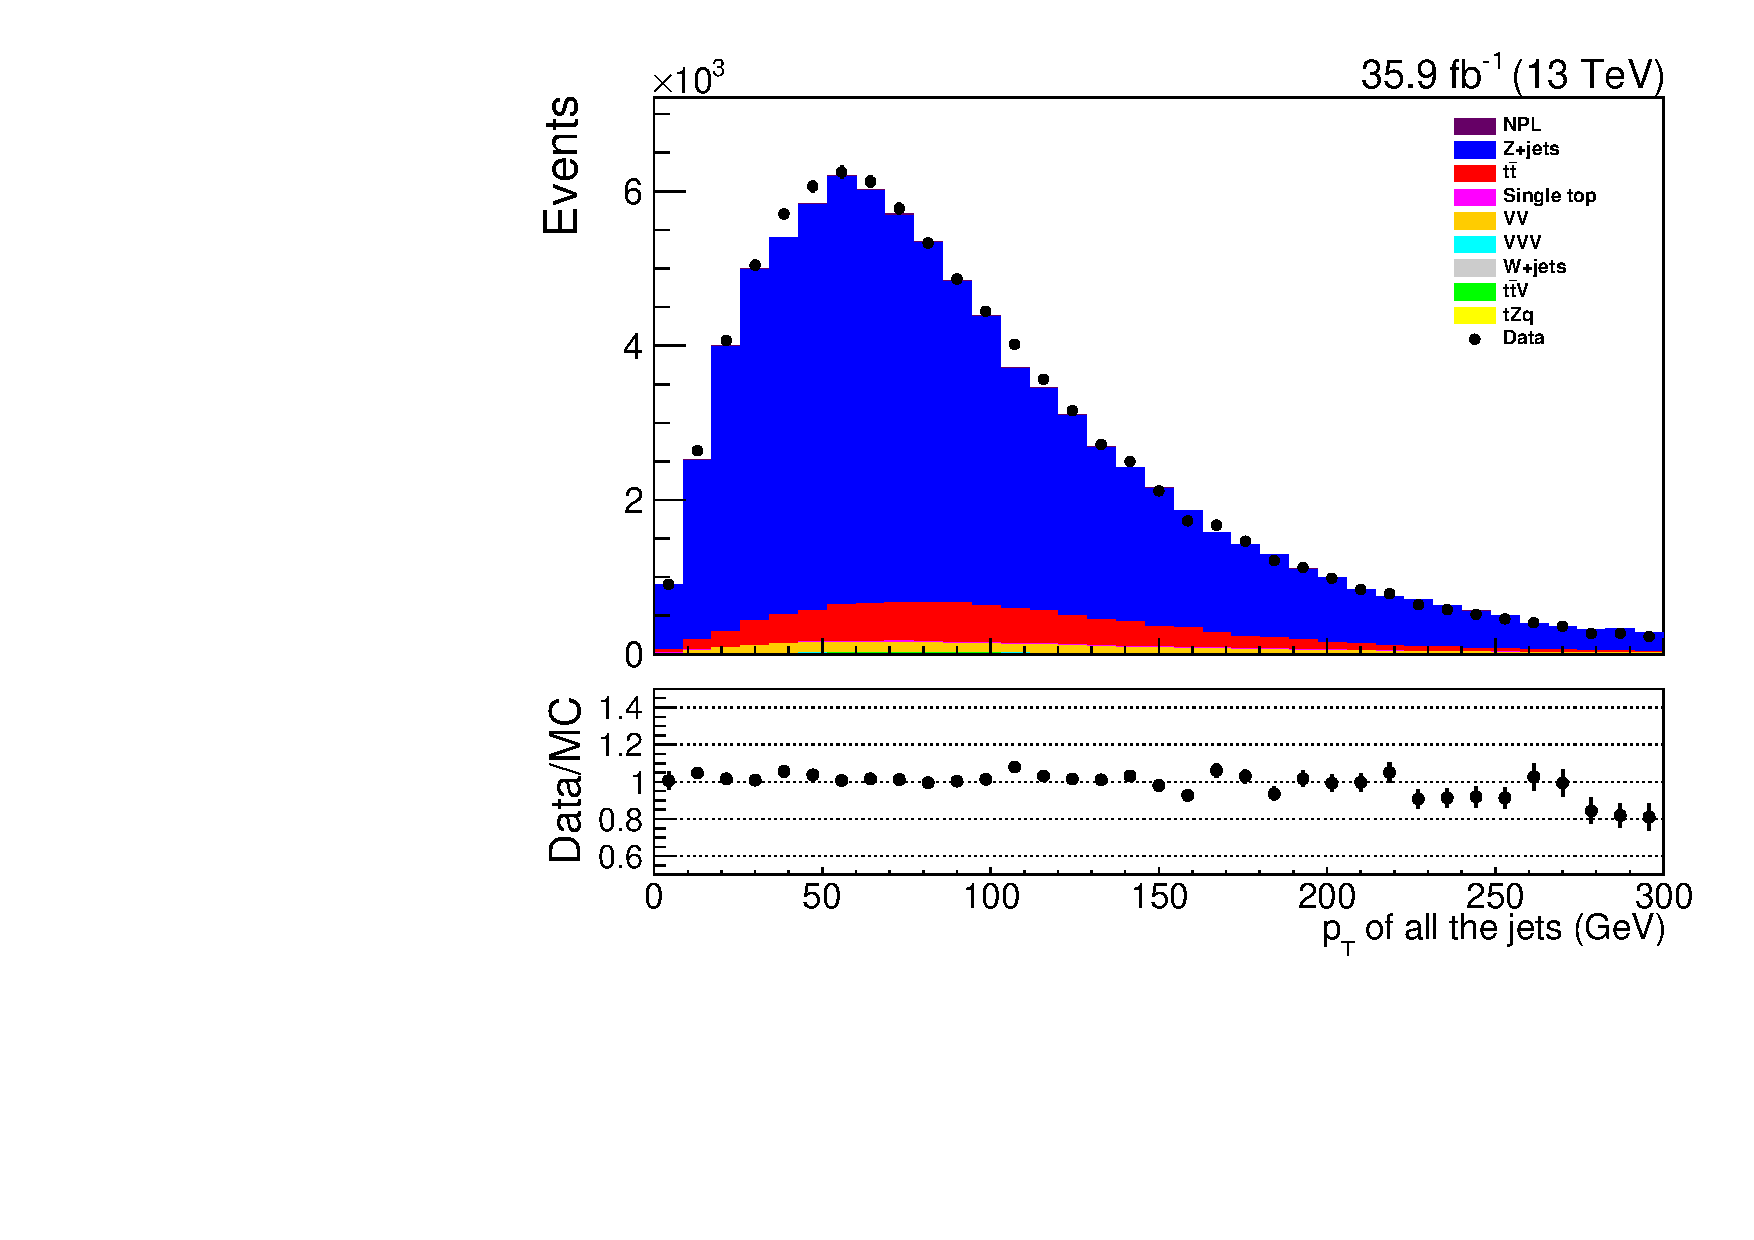
\includegraphics[width=0.47\textwidth]{figs/background-estimation/plots/unblinded/prompt_mumu_ttbarInc/totalJetPt_NPL_mumu_jetSel_mumu.pdf}
\caption{
The distributions of the invariant \pT of all the jets in an event for the $ee$ and $\mu\mu$ channels, left and right respectively, following the application of the jet selection criteria and corrections.
}
\label{fig:SR_totJetPt}
\end{figure}

\begin{figure}[h]
\centering
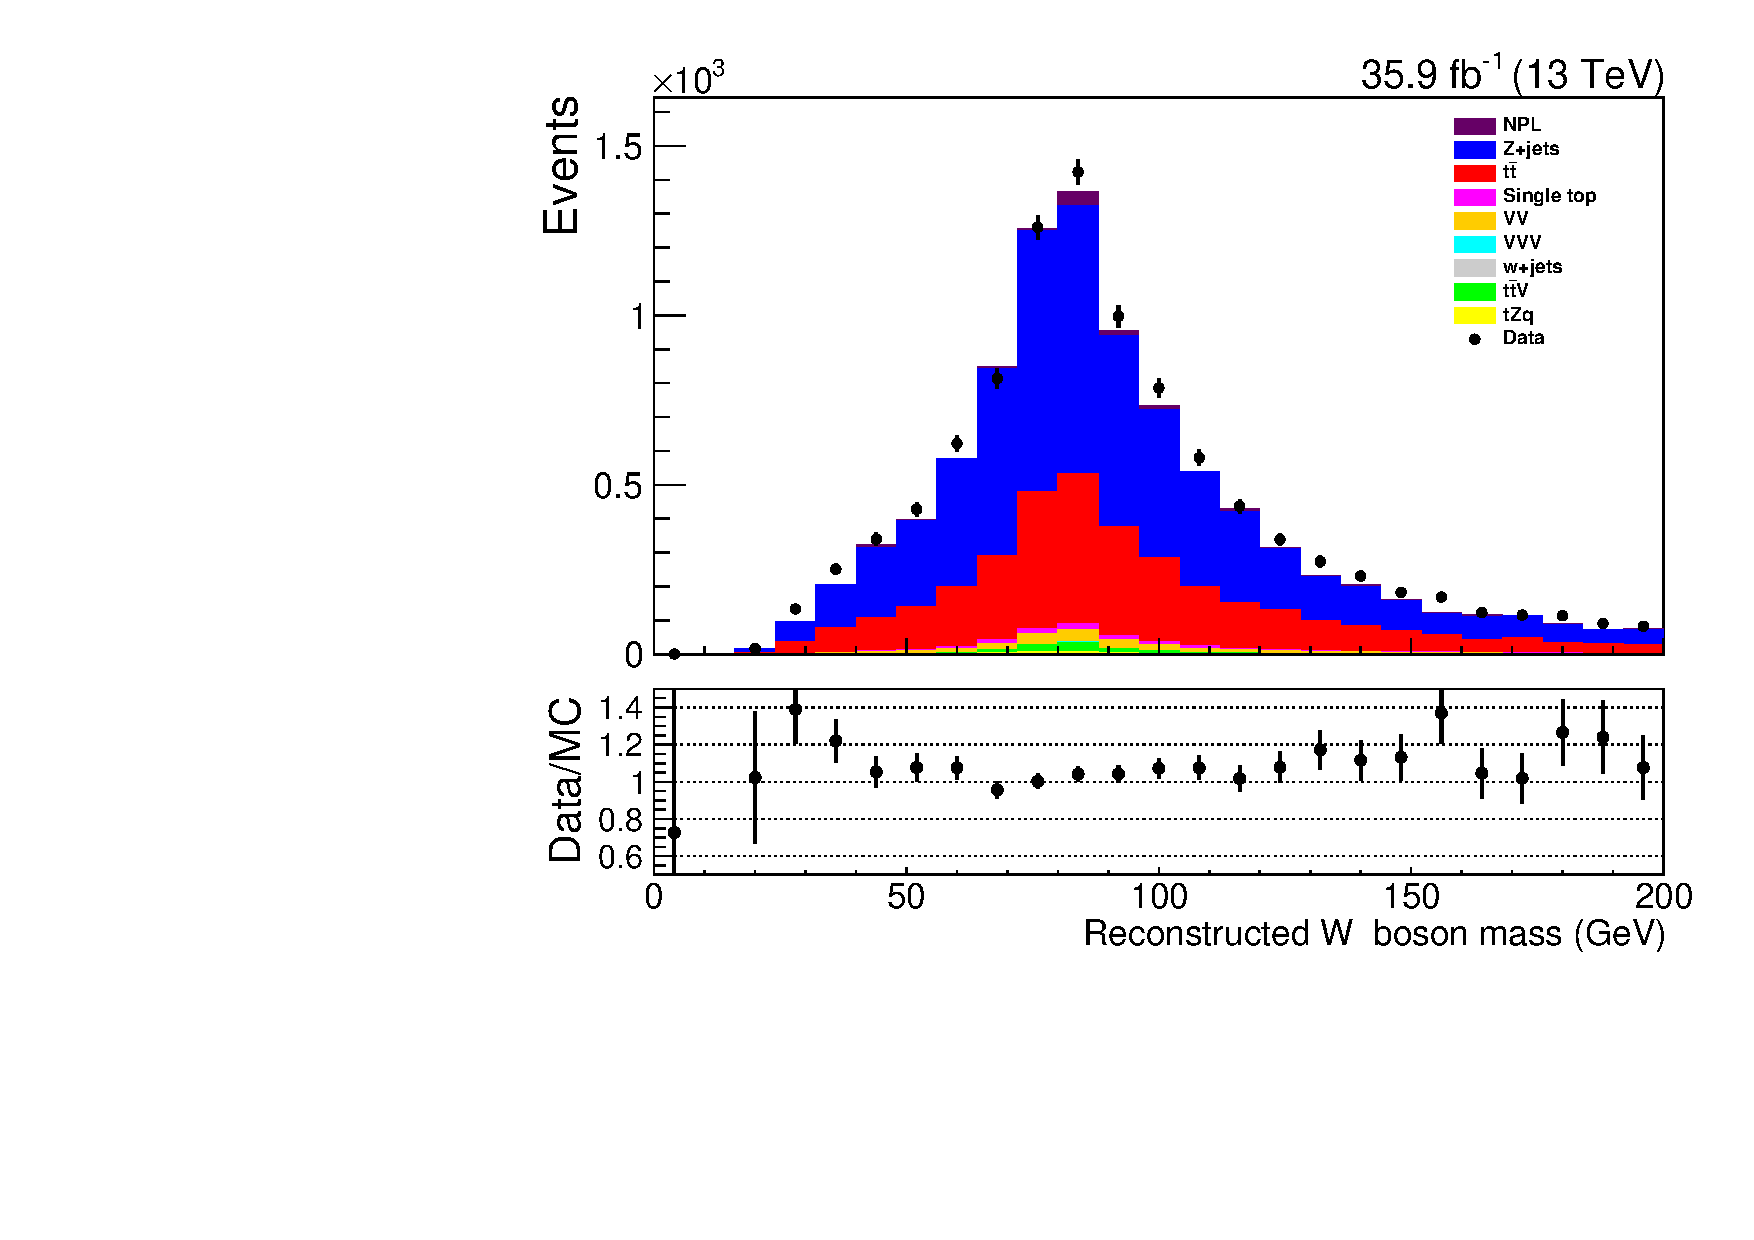
\includegraphics[width=0.47\textwidth]{figs/background-estimation/plots/unblinded/prompt_ee_ttbarInc/wPairMass_NPL_ee_bTag_ee.pdf}
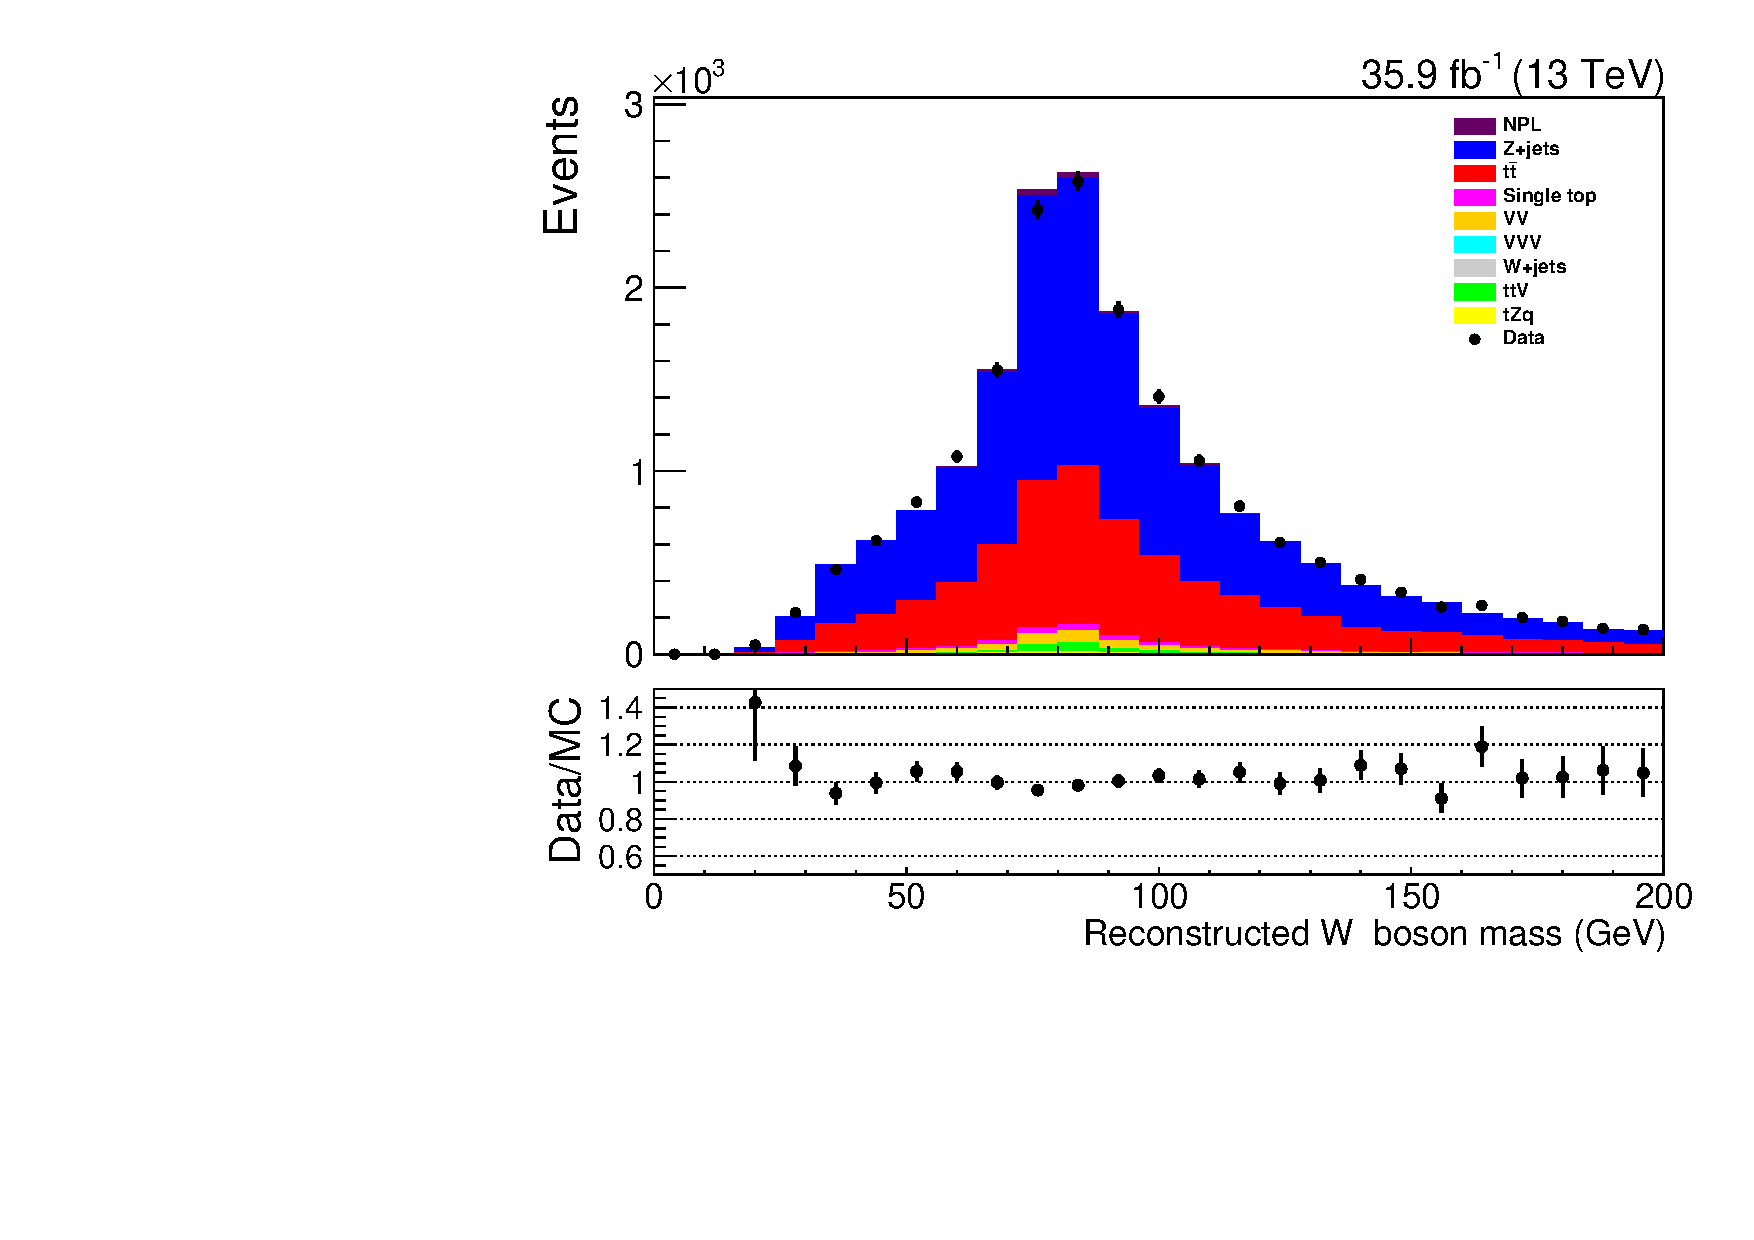
\includegraphics[width=0.47\textwidth]{figs/background-estimation/plots/unblinded/prompt_mumu_ttbarInc/wPairMass_NPL_mumu_bTag_mumu.pdf}
\caption{
The distributions of the reconstructed W boson mass for the $ee$ and $\mu\mu$ channels, left and right respectively, following the application of all the event selection criteria and selections except the W boson mass cut.
}
\label{fig:SR_wBoson}
\end{figure}

%A larger selection of data and simulation comparison plots for both the $ee$ and $\mu\mu$ channels is provided in Appendix~\ref{app:plots}.

\section{Data-driven Background Estimation}\label{sec:dataDrivenBackground}

\subsection{Non-Prompt Leptons}\label{sec:NPLs}
Leptons that are produced from events where at least one jet is incorrectly reconstructed as a lepton (predominately electrons) or a lepton from the decay of heavy quarks (predominately muons) are known as \emph{non-prompt leptons} (NPLs).
The majority of these events are produced by semi-leptonic \ttbar decays, and W+jets production, with smaller contributions from QCD and single top production.
As it is difficult to accurately model QCD processes the NPL contribution is estimated with data.

This data-driven estimate is based on the methodology used in top quark pair production~\cite{CMS:2016syx} and same charge SUSY searches~\cite{CMS:2015vqc}.
This approach takes advantage of the fact that the vast majority of events containing same charge lepton pairs result from non-prompt and charge misidentified leptons, with some contributions from prompt leptons (such as \ttV).
As these backgrounds are independent of the charge of the lepton pairs, it is expected that the nominal opposite charge event selection would have a contribution with a similar magnitude.

Thus, by inverting the signal region's opposite charge lepton pair requirement (\ie by requiring the leptons to have the same, not opposite, charge), a same sign control region can be defined that is dominated by NPL events while containing a small admixture of from prompt lepton events, charge misidentification and real same charge lepton pairs.

Using this control region, a data-driven estimate of the contribution of opposite charge NPLs can be derived as follows:

\begin{equation}\label{eq:NPL}
N_{data}^{OS non-prompt} = (N_{data}^{SS} - N^{SS}_{real + mis-ID}) \cdot \frac{N_{MC}^{OS non-prompt}}{N_{MC}^{SS non-prompt}}
\end{equation}

where $N_{data}^{SS}$ is the total number of same sign events observed in data and $N^{SS}_{real + mis-ID}$ is the expected number of real same sign events and events with charge misidentification.

The ratio of opposite sign and same sign NPLs in simulation, $N_{MC}^{OS non-prompt}$ and $N_{MC}^{SS non-prompt}$, respectively, is used to appropriately normalise this estimate and uses the generator level information in simulation to correctly identify how the leptons were produced.
The W+jets, \ttZ, \ttW, and single top simulated samples that have sufficient statistics in the same sign control region are used to calculate this ratio as these simulation indicates that these processes are the predominant source of non-prompt leptons for this analysis.

The event yields of the simulated samples and data following the full event selection in the same lepton sign control region, the same sign background contributions not accounted for by simulation, ratio of same charge to opposite charge event yields and the data-driven NPL contribution estimate are given in table~\ref{tab:fakeLeptonYields}.

\begin{table}[htbp]
\topcaption{The event yields following the full event selection ratio of same to opposite charge lepton events, the same sign background contributions not accounted for by simulation, ratio of same charge to opposite charge event yields and the estimated non-prompt lepton contribution following all selection cuts.
}
\centering
\begin{tabular}{l | cccc}
\hline
Source &  $ee$ & $\mu\mu$  \\ 
\hline
$N_{\ttbar}^{SS}$ & 5.85 $\pm$ 1.30 & 8.93$\pm$1.47    \\
$N_{\ttbar V}^{SS}$ & 4.81 $\pm$ 0.11 & 11.81 $\pm$0.10  \\ 
$N_{single top}^{SS}$ & 0.90$\pm$0.18 & 0.97 $\pm$0.11    \\
$N_{W+jets}^{SS}$ & 0.0$\pm$0.0 & 0.0 $\pm$ 0.0  \\
$N_{Z+jets}^{SS}$ & 37.53$\pm$6.85 & 0.0 $\pm$ 0.0  \\
$N_{VV}^{SS}$ & 1.89$\pm$0.22 & 0.35$\pm$0.13 \\
$N_{VVV}^{SS}$ & 0.00$\pm$ & 0.23$\pm$0.09 \\
\hline
$N_{MC}^{SS}$ background & 50.98$\pm$6.98 & 22.29 $\pm$ 2.21 \\ 
$N_{data}^{SS}$ & 126.0 $\pm$ 11.22 & 125.0 $\pm$ 1.18\\ 
\hline
$N_{data}^{SS} - N_{MC}^{SS}$: & 30.64$\pm$13.21 & 102.71 $\pm$ 6.27\\
\hline
$N_{MC}^{OS non-prompt}$: & 1.58$\pm$0.03 & 2.38$\pm$0.04 \\
$N_{MC}^{SS non-prompt}$: & 1.71$\pm$0.03 & 2.14$\pm$0.04 \\
$N_{MC}^{OS non-prompt}/N_{MC}^{SS non-prompt}$: & 0.93 $\pm$ 0.02 & 1.11 $\pm$ 0.03 \\
\hline
$N_{data}^{OS non-prompt}$: & 69.47$\pm$12.95 & 114.01$\pm$7.61 \\
\hline
\end{tabular}
\label{tab:fakeLeptonYields}
\end{table}

\subsection{Z+jets Background}\label{subsec:zPlusJetsEstimation}
In Section~\ref{subsec:zPlusJetsCR} two Z+jets enriched control regions were defined to produce orthogonal regions that were topologically similar to the signal region to validate the modelling of the simulated Z+jets samples.
These control regions differed from the signal region by either requiring zero b-tagged jets in the event (0-bjet) or an inverted W boson mass threshold and less than 50\GeV of \MET is present in an event ($m_{W}^{inv}$).

Two different simulated samples were considered for modelling the Z+jets processes: one generated at LO and the other at NLO.
Given that the final state of the signal process contains multiple jets, it would be preferable to use the NLO description of this large multi-jet background.
Both of these samples are listed in table~\ref{tab:mcList}.

The final event yields for the 0-bjet region are given in table~\ref{tab:zPlusControlYieldsOld} and the corresponding yields for the $m_{W}^{inv}$ region are given in table~\ref{tab:zPlusControlYieldsNew}.
It was observed that 94\% of the simulated events in the 0-bjet region were produced by Z+jets processes compared to 82\% in the $m_{W}^{inv}$ region.
Consequently, it was decided to use the 0-bjet region to validate the modelling of the Z+jets processes.

\begin{figure}[!h]
\centering
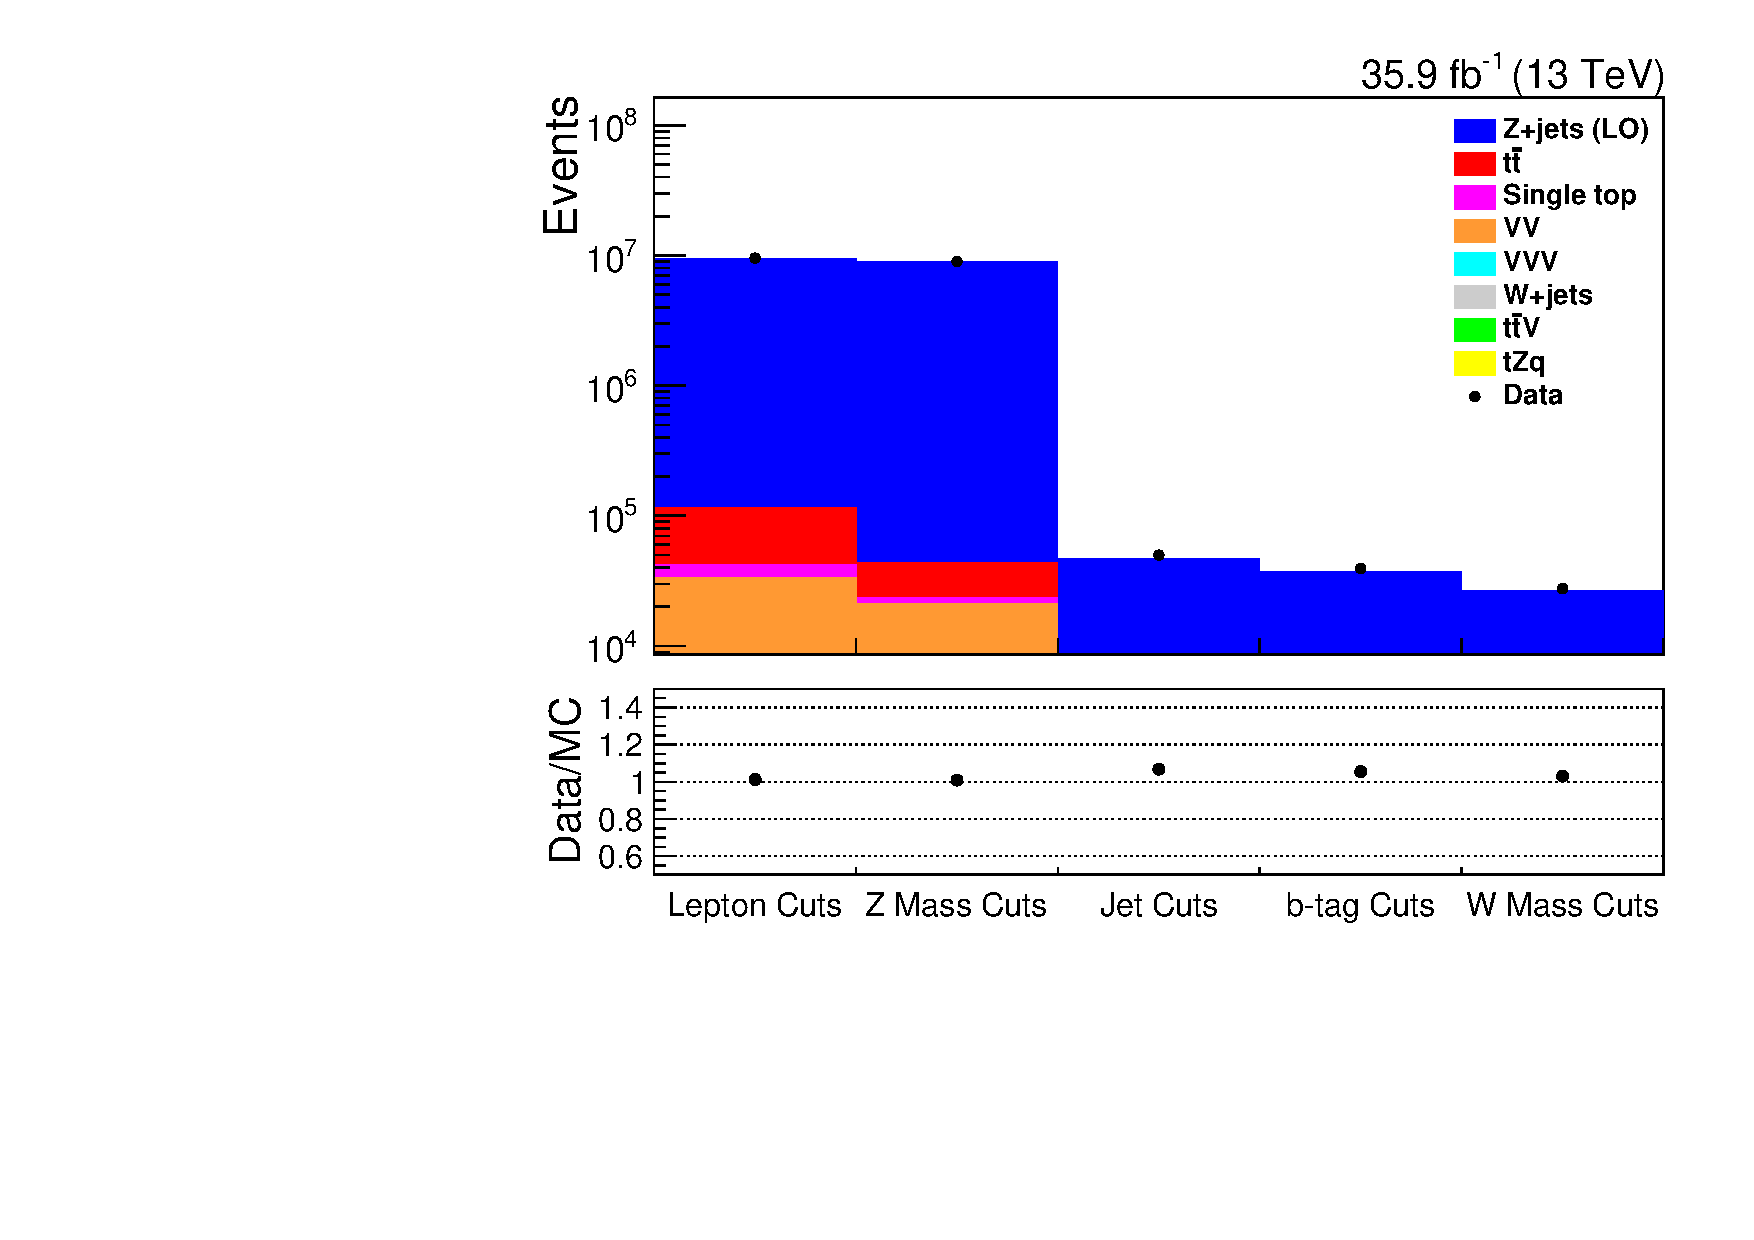
\includegraphics[width=0.47\textwidth]{figs/background-estimation/plots/unblinded/DY_control_old_prompt_ee_ttbarInc/cutFlow_log.pdf}
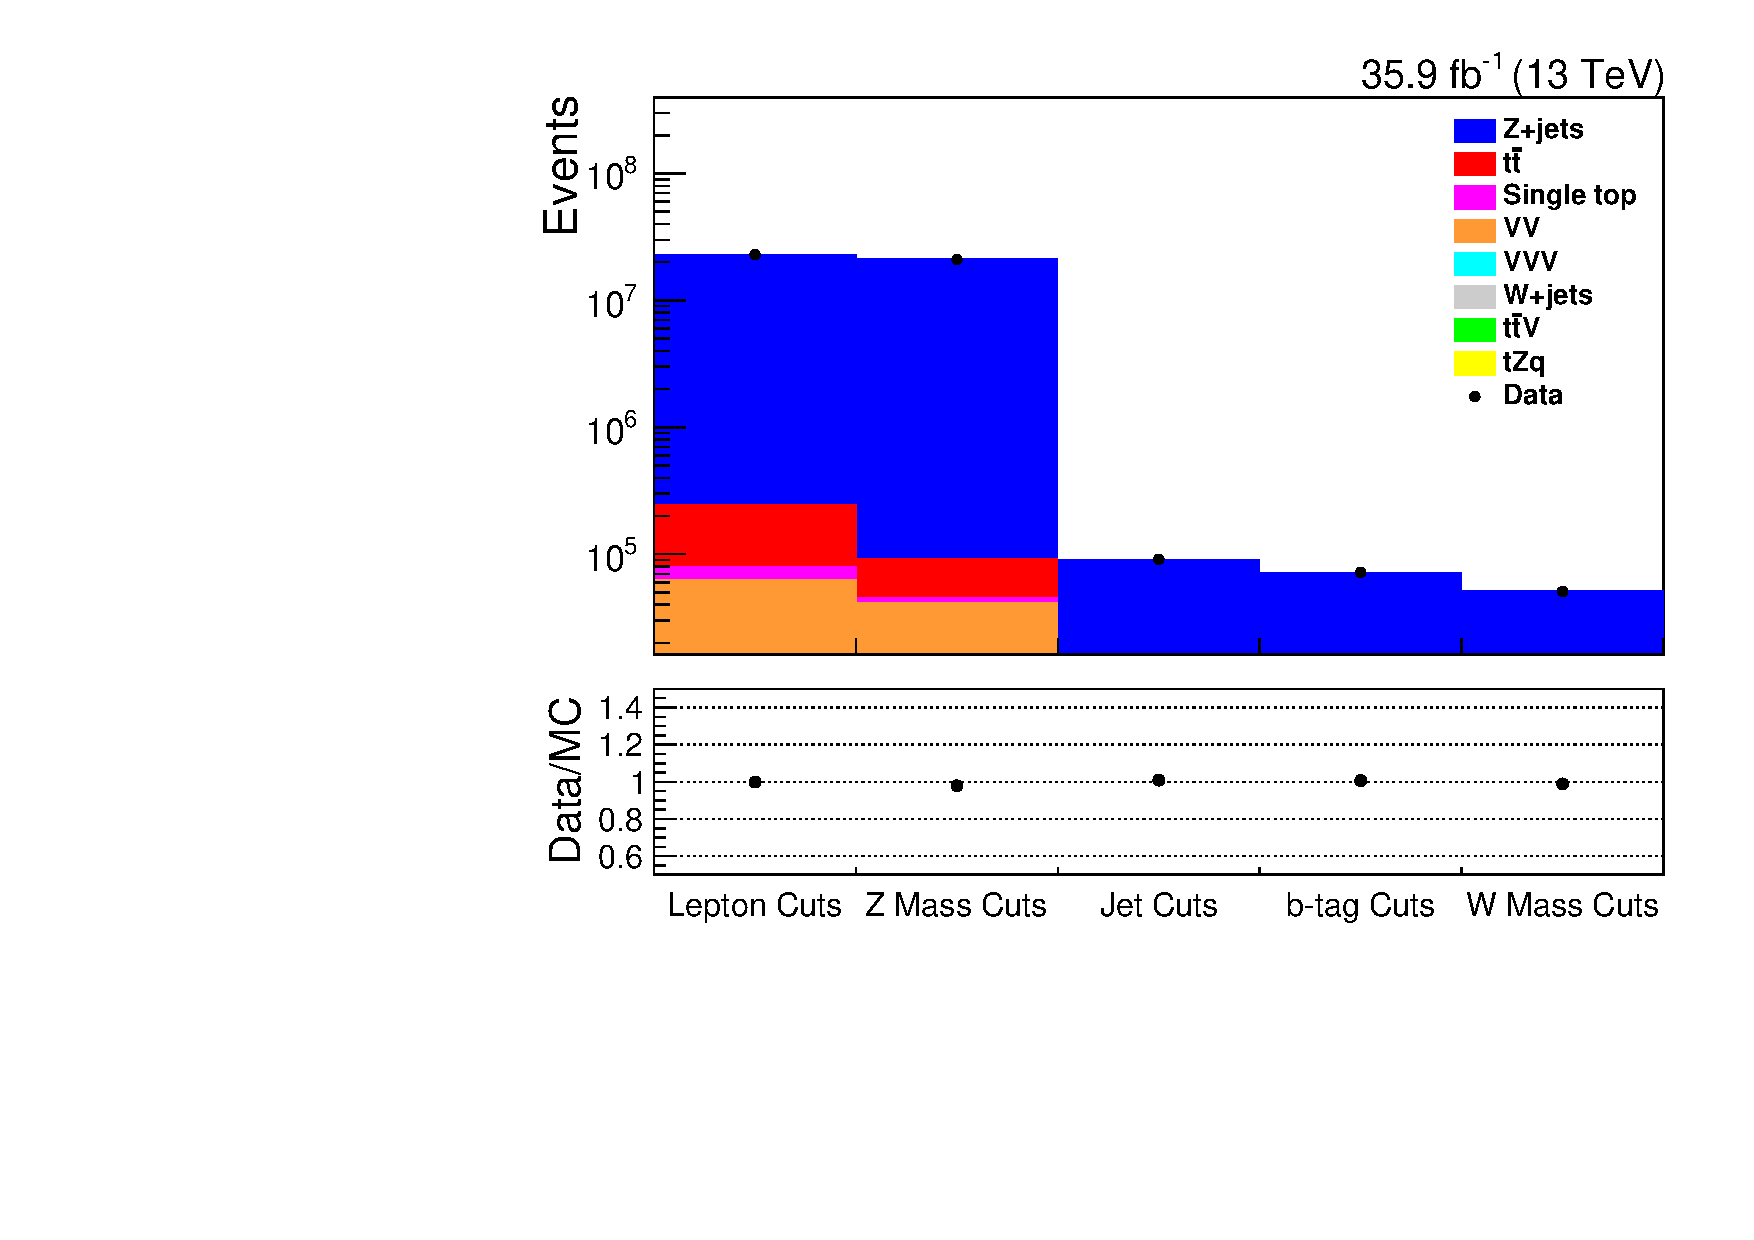
\includegraphics[width=0.47\textwidth]{figs/background-estimation/plots/unblinded/DY_control_old_prompt_mumu_ttbarInc/cutFlow_log.pdf}
\\
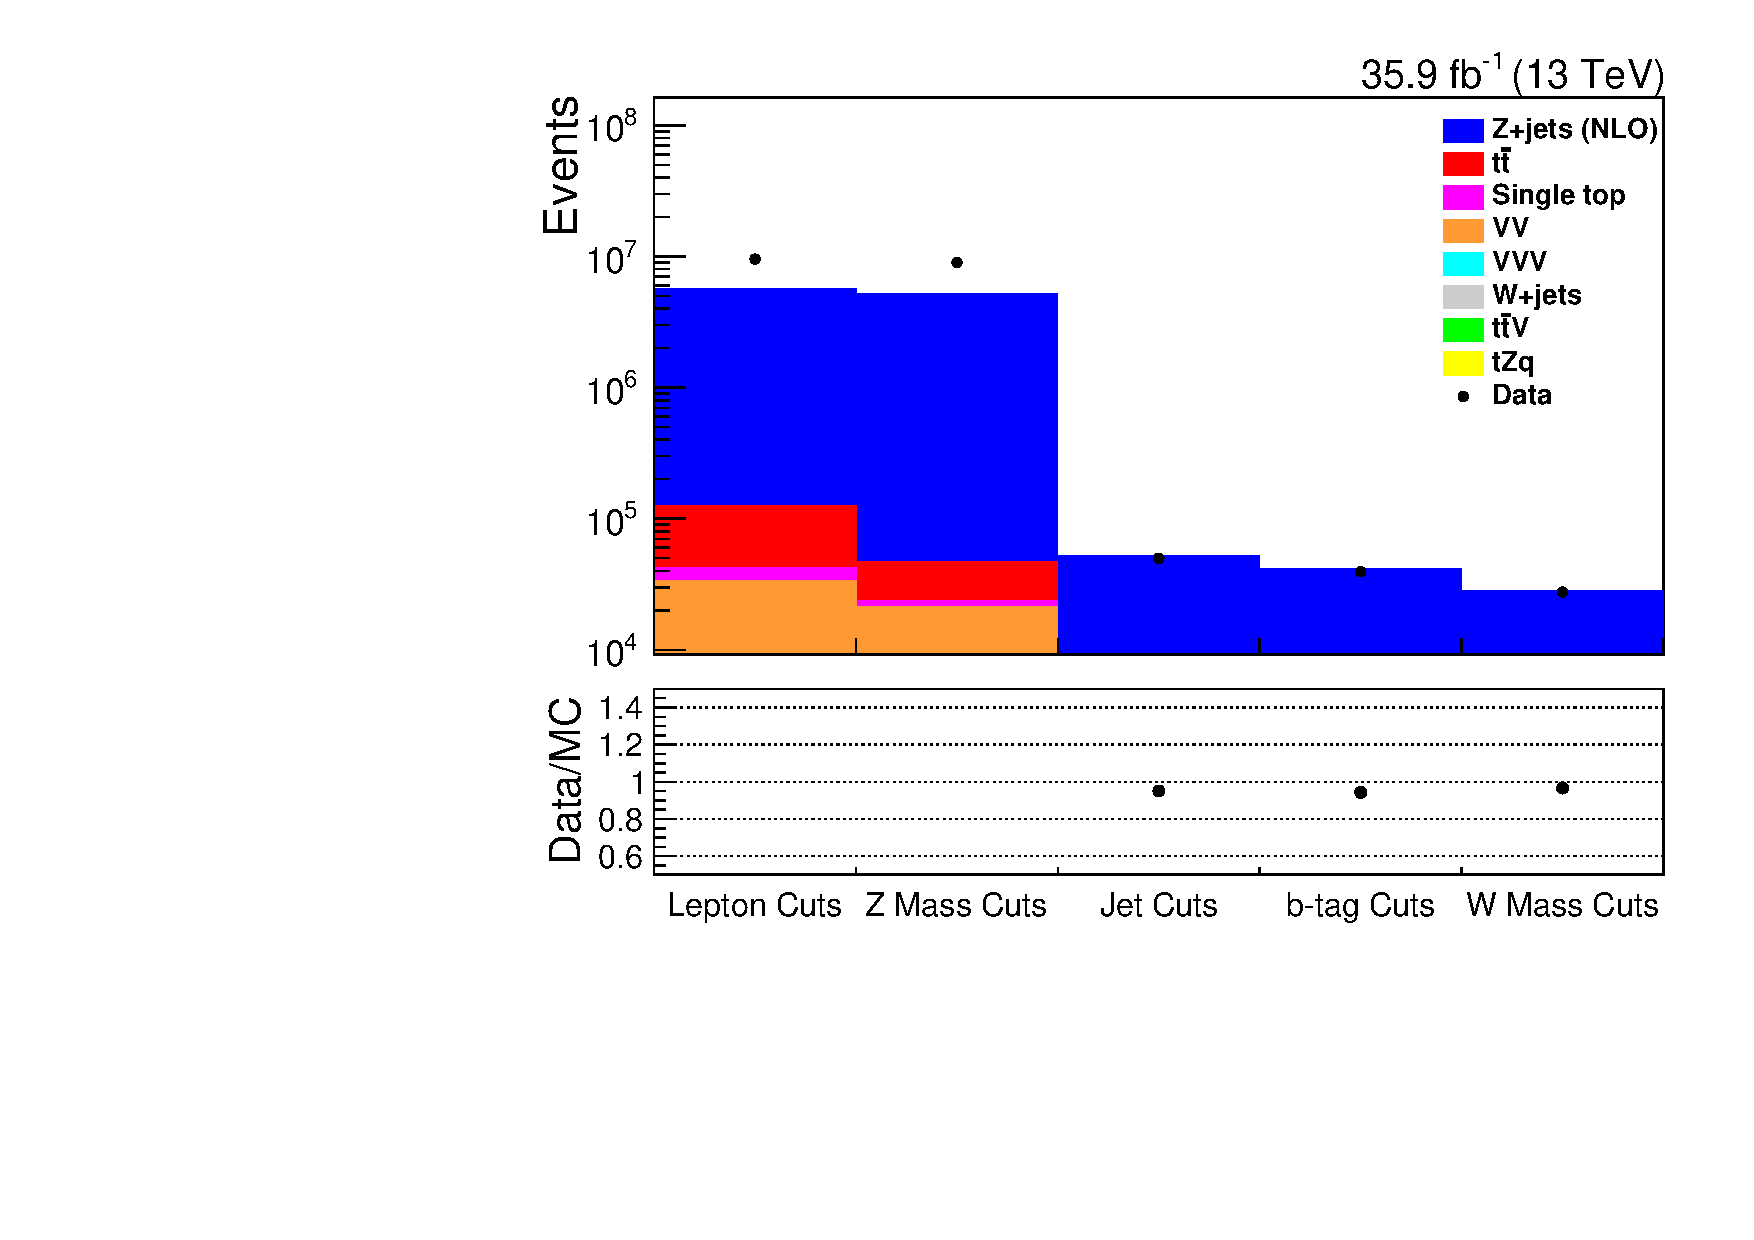
\includegraphics[width=0.47\textwidth]{figs/background-estimation/plots/unblinded/DY_control_old_prompt_ee_DYamcatnlo/cutFlow_log.pdf}
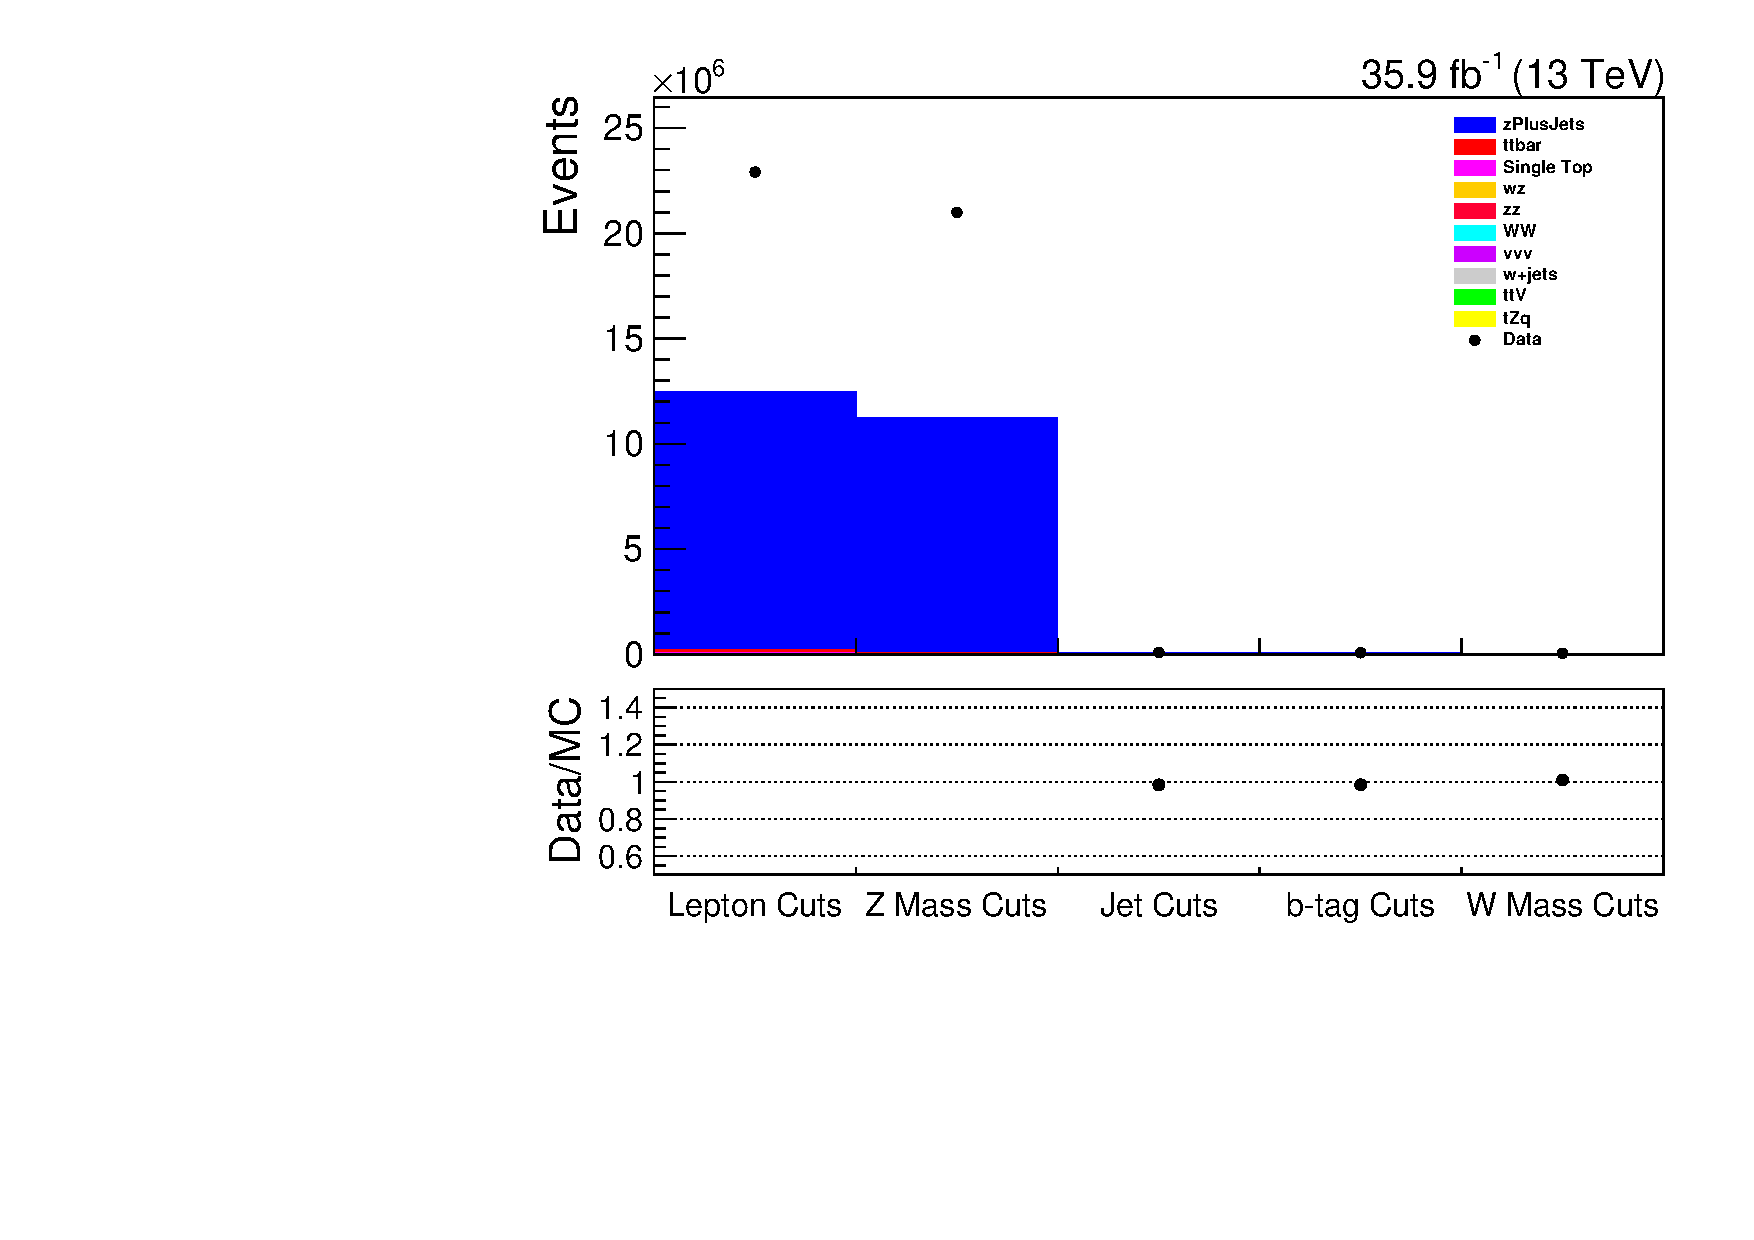
\includegraphics[width=0.47\textwidth]{figs/background-estimation/plots/unblinded/DY_control_old_prompt_mumu_DYamcatnlo/cutFlow_log.pdf}
\caption{
The overall event yield for data and simulation at each stage of applying the 0-bjet region selection criteria and simulation corrections for when the LO (top) and NLO (bottom) simulation samples are used to model the Z+jets processes.
The event yields for the $ee$ channel and the $\mu\mu$ channel are shown on the left and right, respectively.
}
\label{fig:zPlus_cutFlow}
\end{figure}

Based on the final event yields in both control regions, as given in tables~\ref{tab:zPlusControlYieldsOld}-\ref{tab:zPlusControlYieldsNew}, it was observed that the NLO Z+jets sample did not correctly describe the normalisation of the Z+jets process.
Further studies into the NLO Z+jets sample were done using a simple scale factor based on the final event yields to correctly normalise this Z+jets sample.

During these studies it was found that the NLO Z+jets normalisation scale factor only resolves the incorrect normalisation of this process following the application of the jet selection criteria, as shown in Figure~\ref{fig:zPlus_cutFlow}.
In contrast consistently good agreement is observed at all stages of applying the 0-bjet region selection criteria when the LO Z+jets sample is used.

As illustrated in Figure~\ref{fig:zPlusCR_nJets}, the disagreement that is observed between simulation and data when using the NLO Z+jets sample is the result of the NLO sample incorrectly describing low jet multiplicities.
The LO Z+jets sample however, correctly describes jet multiplicities throughout the application of the 0-bjet region selection criteria selection criteria.

\begin{figure}[!h]
\centering
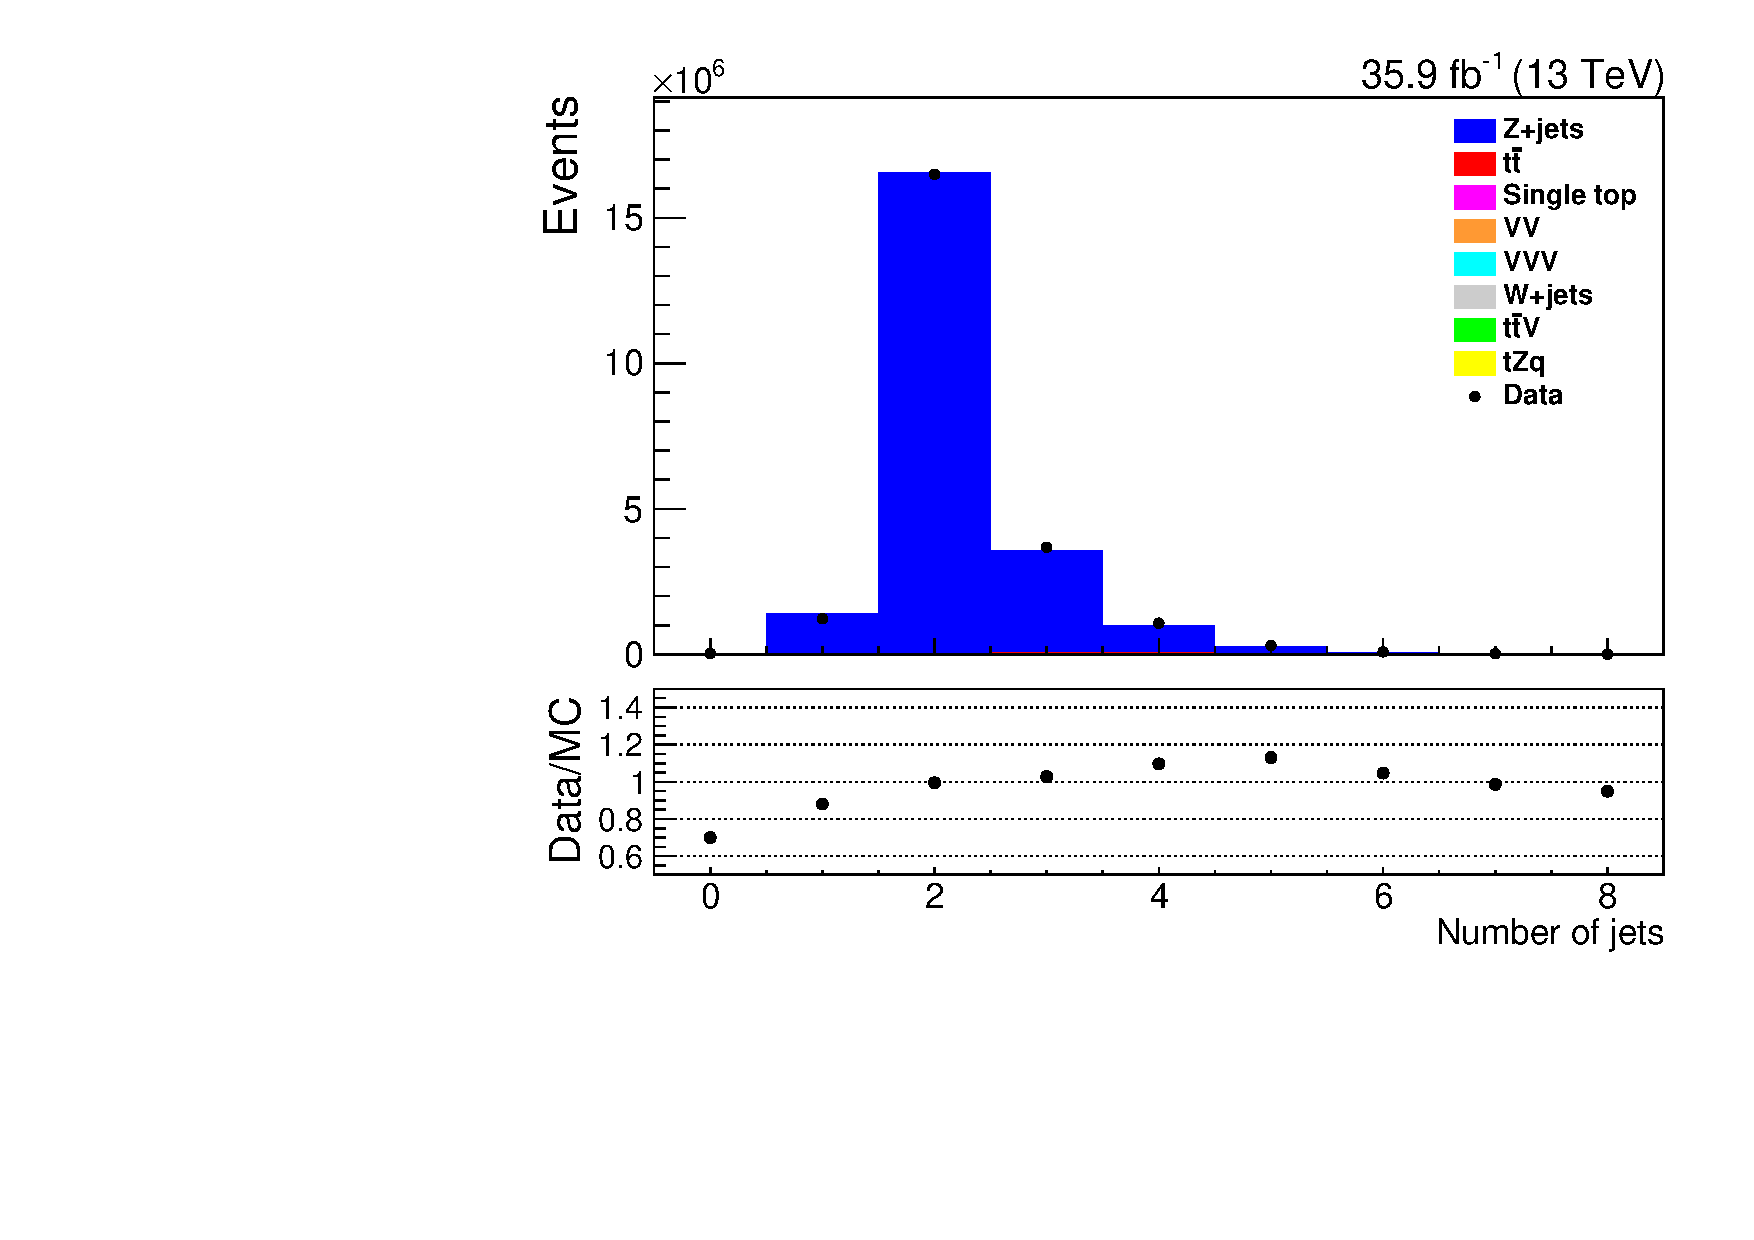
\includegraphics[width=0.47\textwidth]{figs/background-estimation/plots/unblinded/DY_control_old_prompt_mumu_ttbarInc/numbJets_SingleTop_lepSel_mumu.pdf}
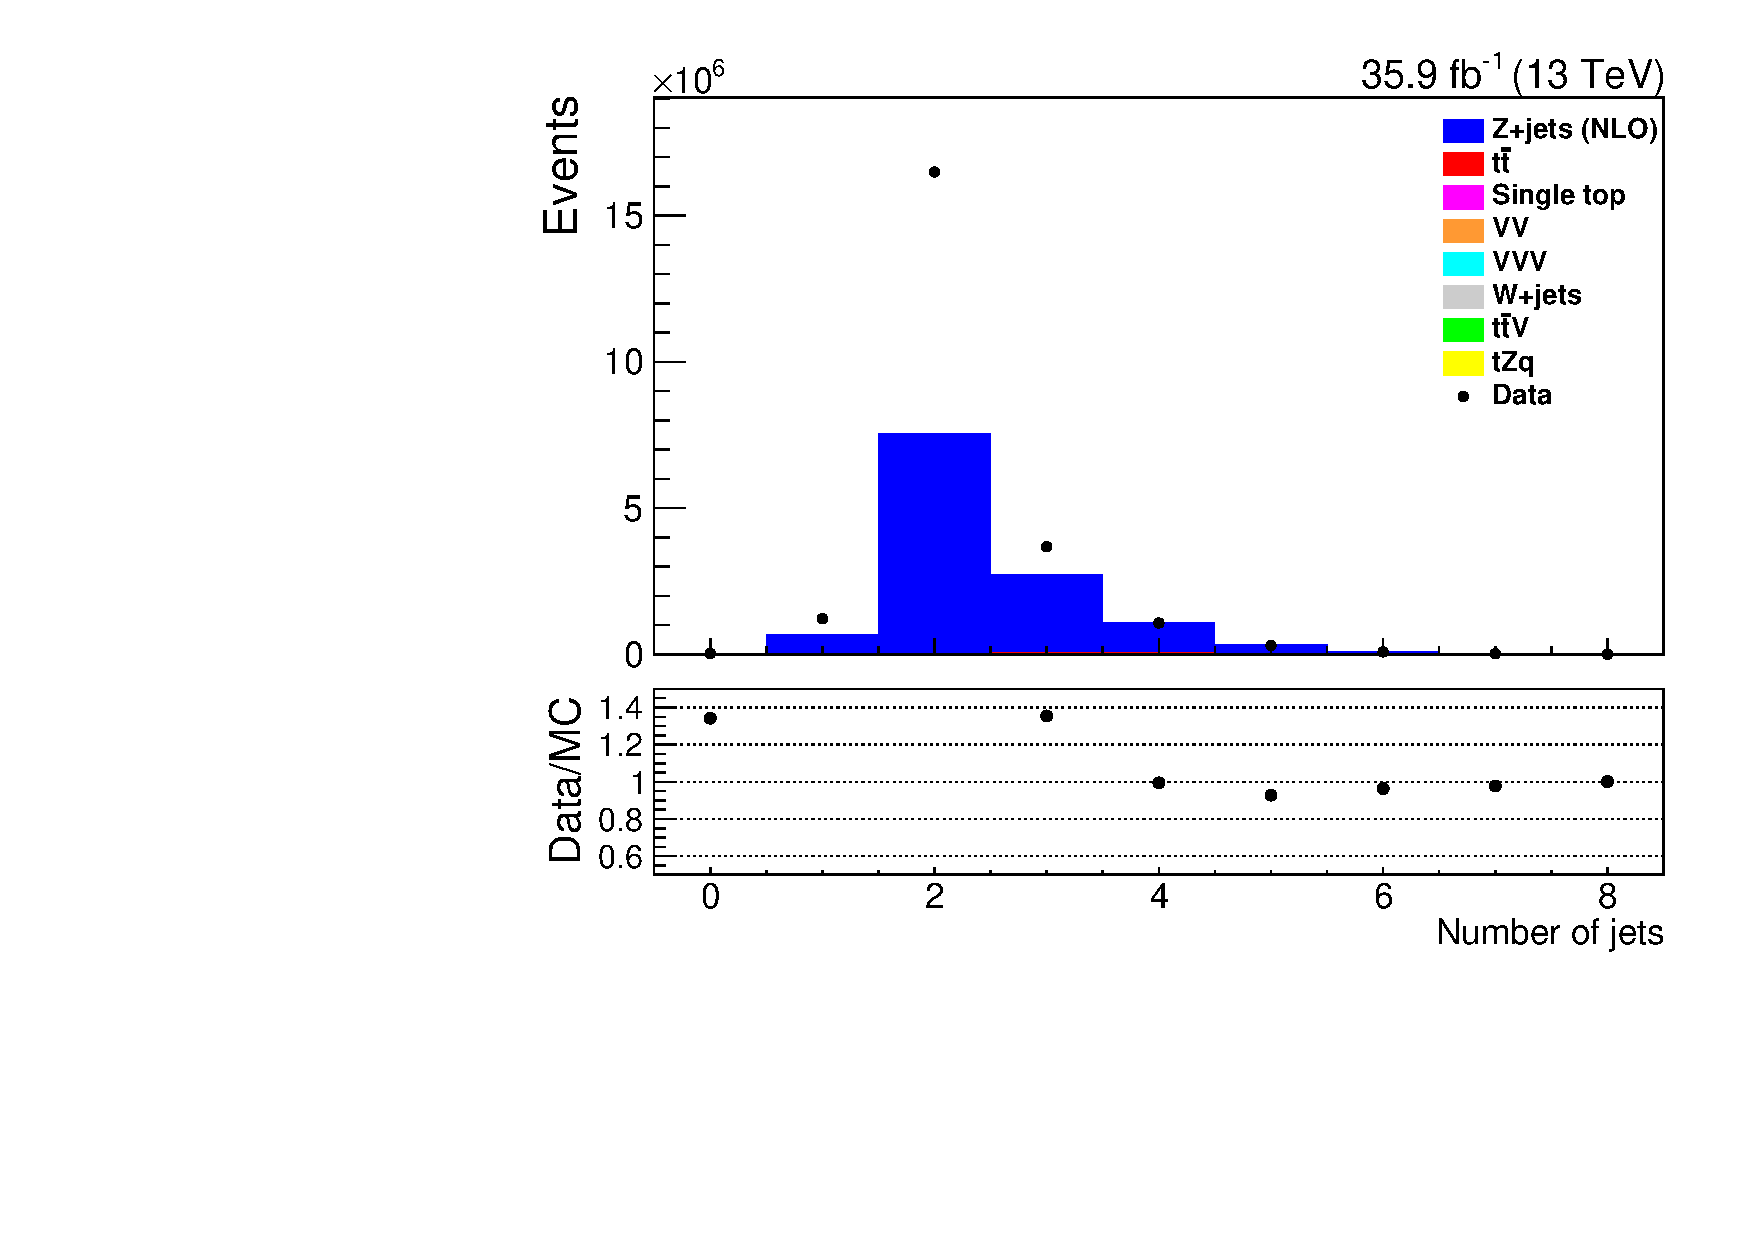
\includegraphics[width=0.47\textwidth]{figs/background-estimation/plots/unblinded/DY_control_old_prompt_mumu_DYamcatnlo/numbJets_SingleTop_lepSel_mumu.pdf}
\caption{
The distributions of the number of jets in the 0-bjet region following the lepton selection criteria and associated simulation corrections for the LO (left) and NLO (right) Z+jets samples in the $\mu\mu$ channel.
}
\label{fig:zPlusCR_nJets}
\end{figure}

\begin{figure}[!hp]
\centering
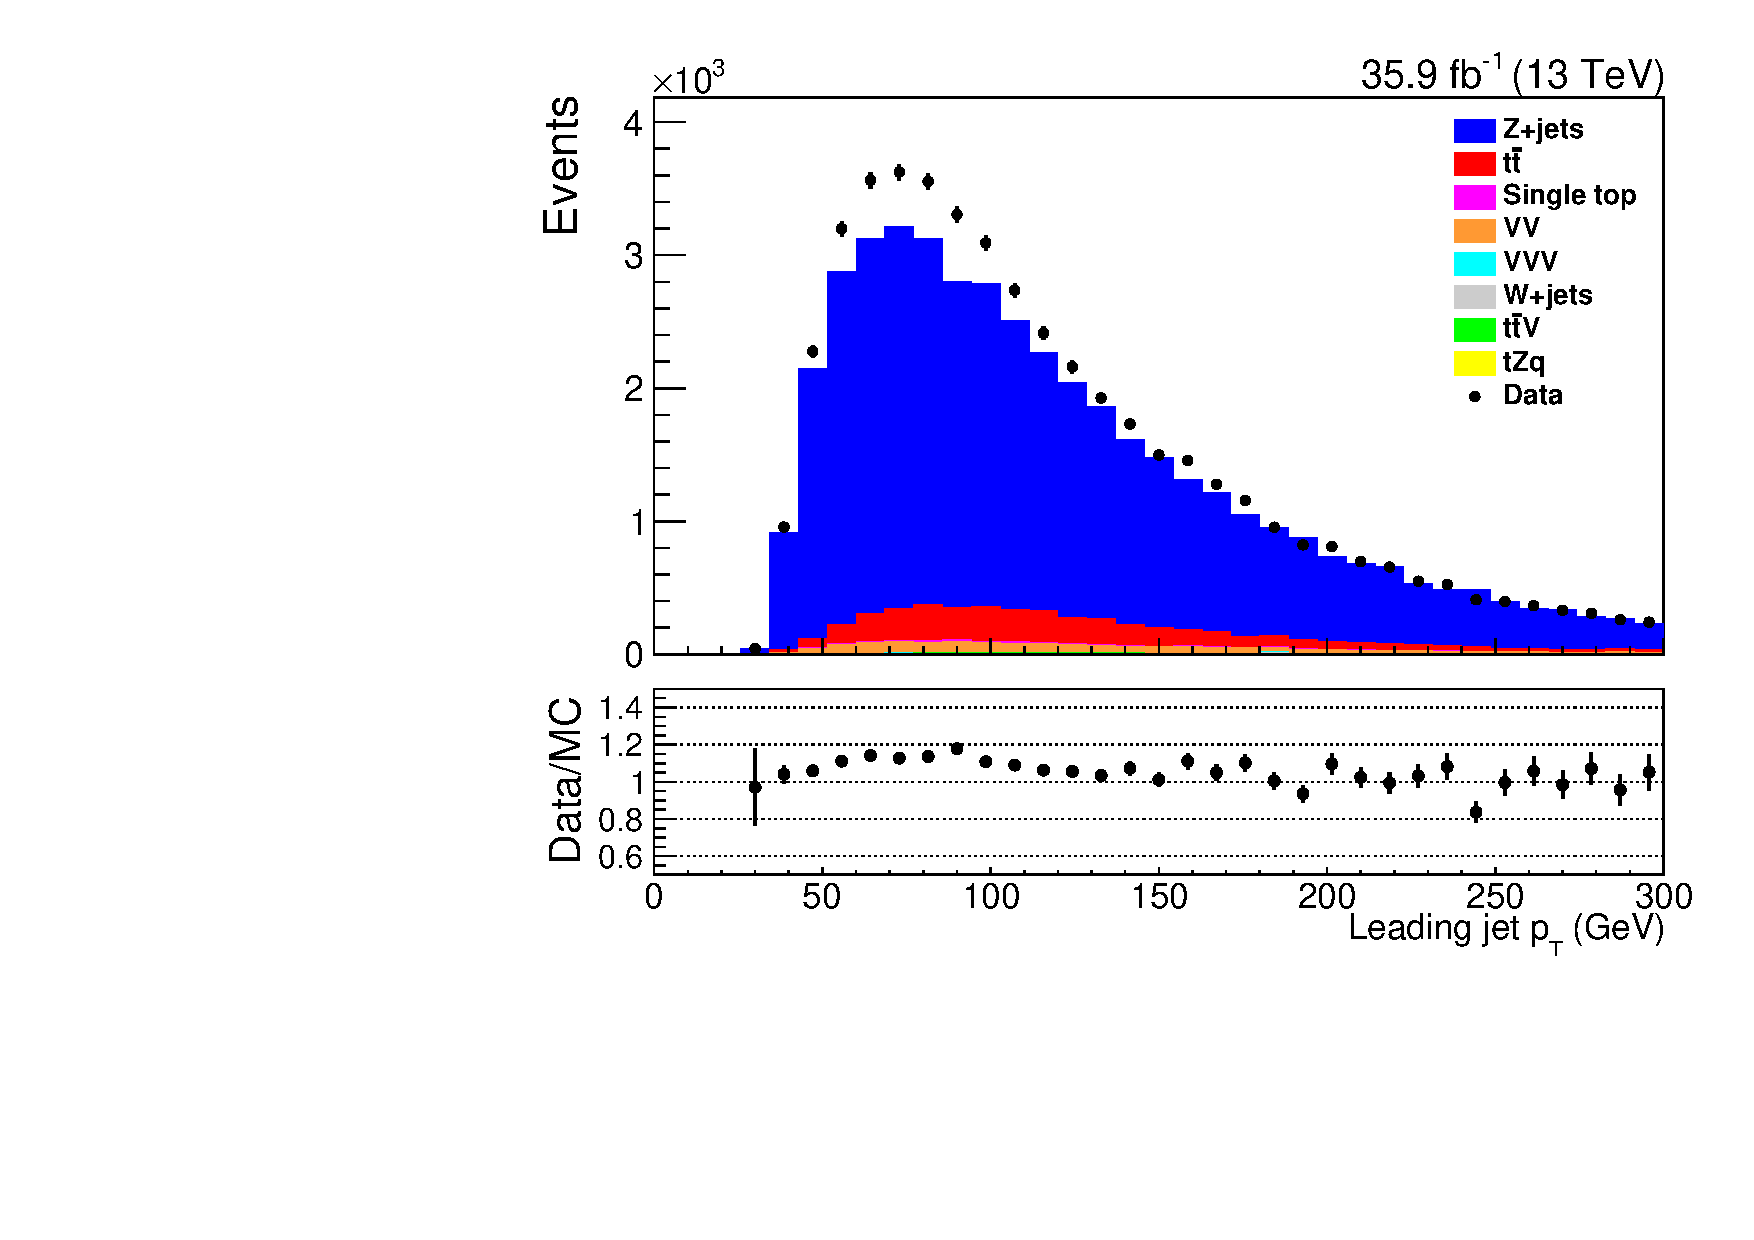
\includegraphics[width=0.47\textwidth]{figs/background-estimation/plots/unblinded/DY_control_old_prompt_ee_ttbarInc/leadingJetPt_SingleTop_jetSel_ee.pdf}
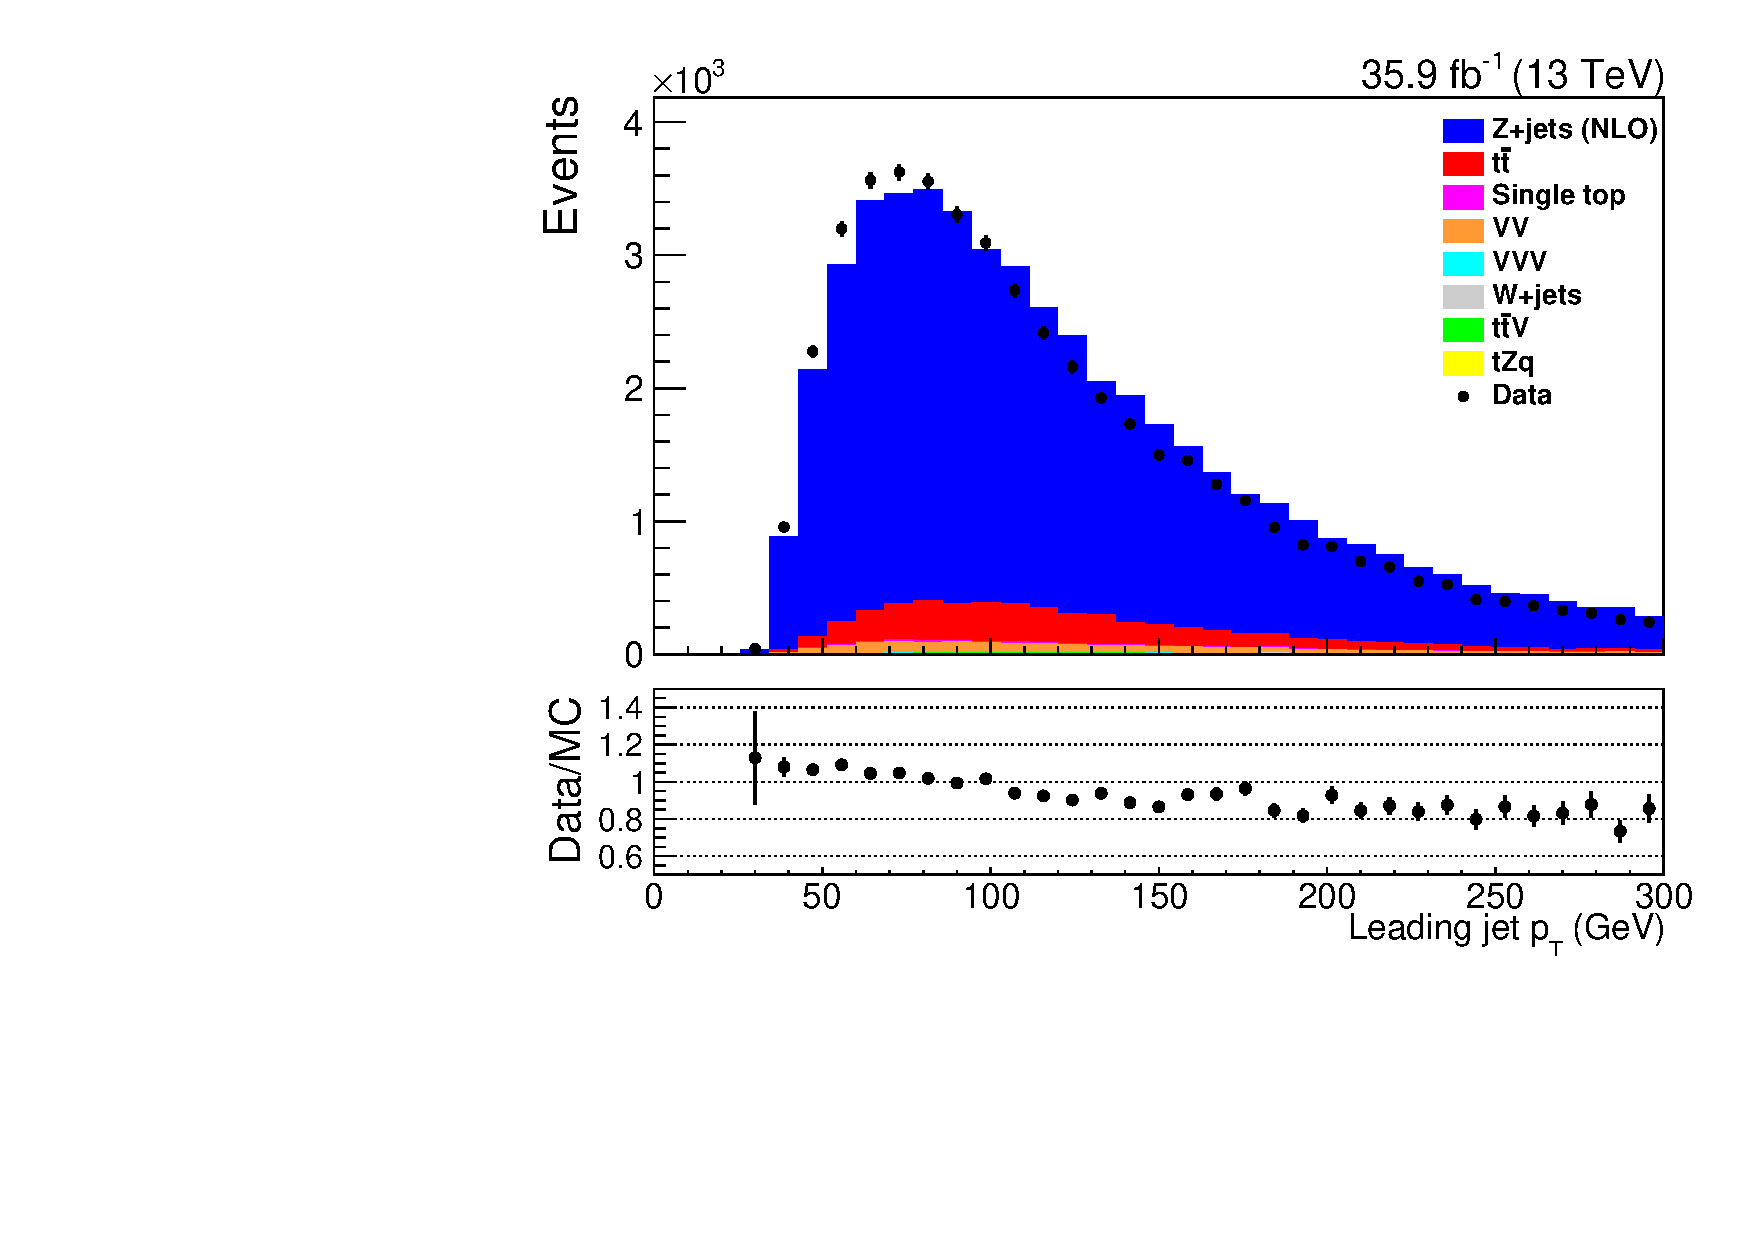
\includegraphics[width=0.47\textwidth]{figs/background-estimation/plots/unblinded/DY_control_old_prompt_ee_DYamcatnlo/leadingJetPt_SingleTop_jetSel_ee.pdf}
\\
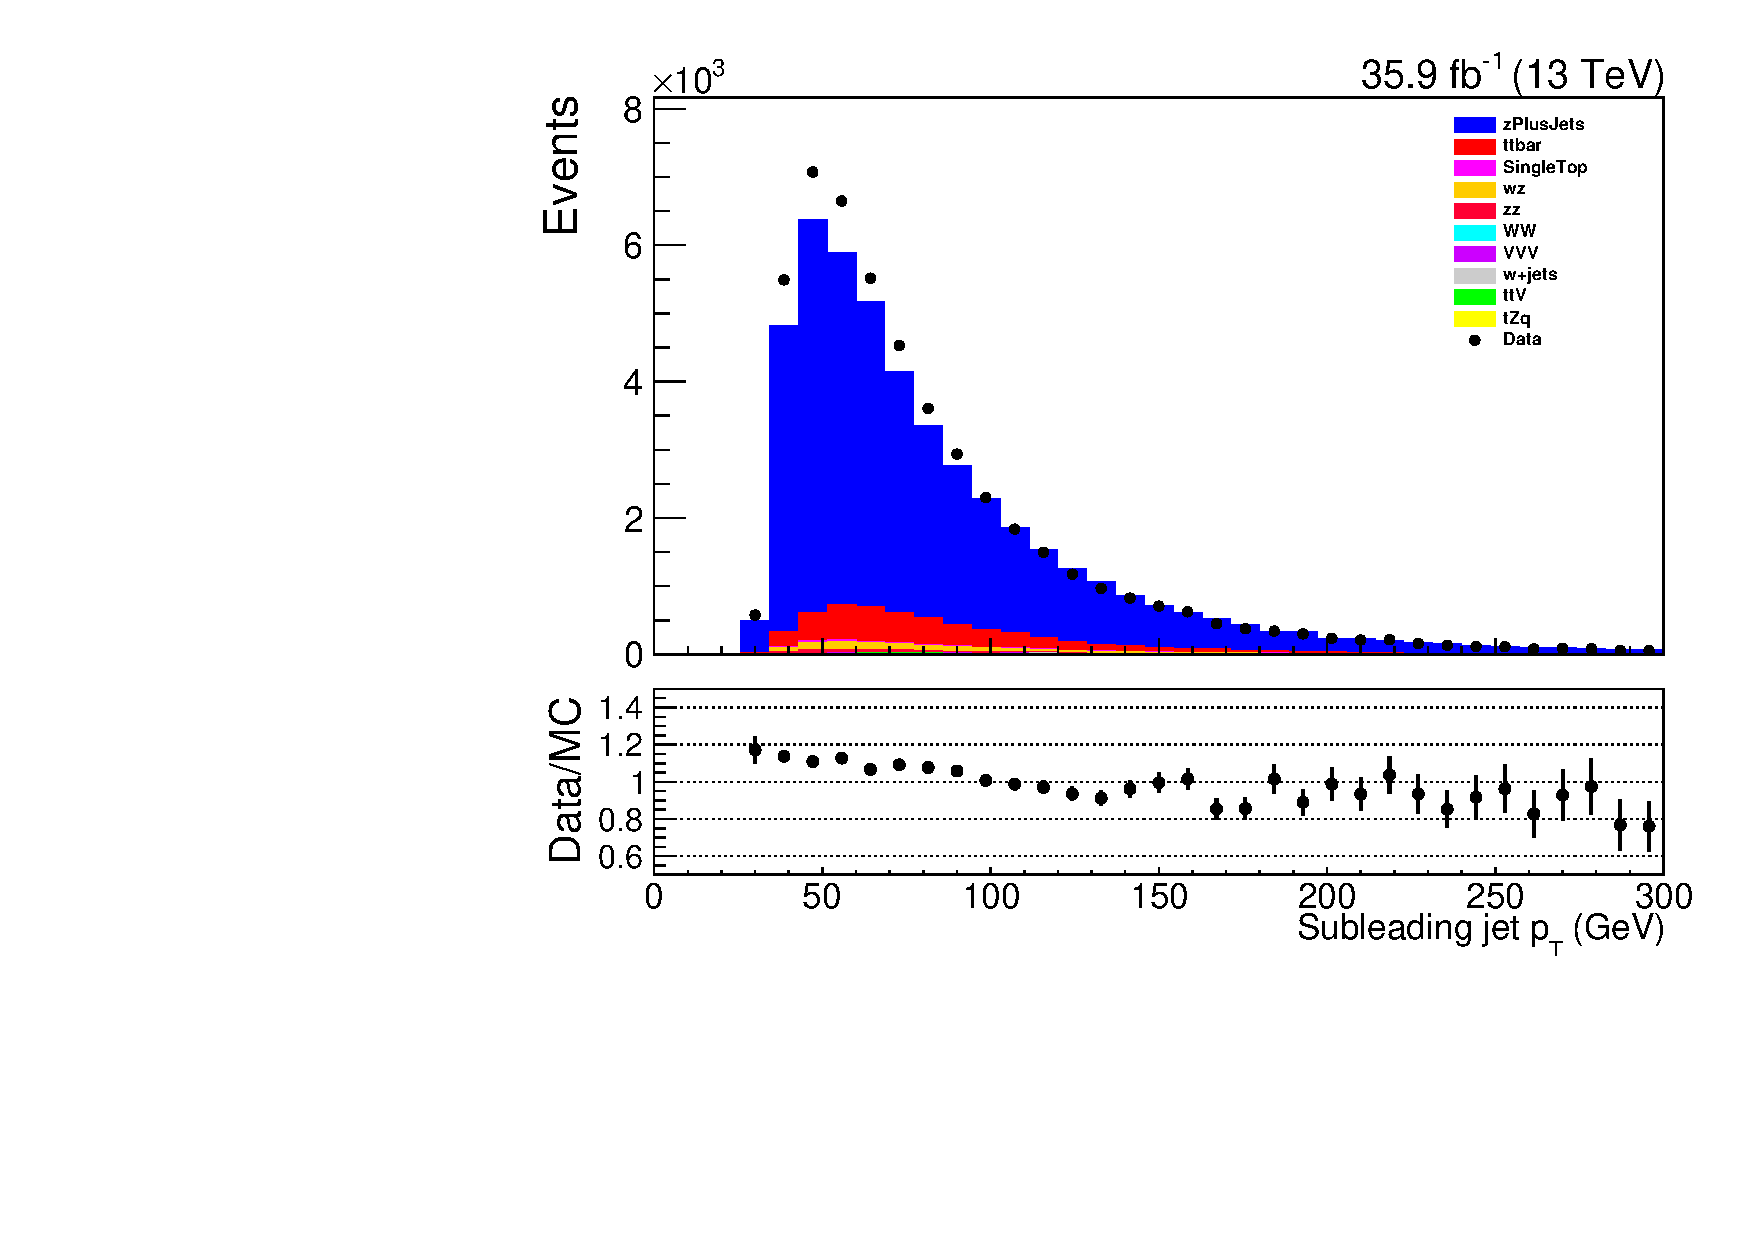
\includegraphics[width=0.47\textwidth]{figs/background-estimation/plots/unblinded/DY_control_old_prompt_ee_ttbarInc/secondJetPt_SingleTop_jetSel_ee.pdf}
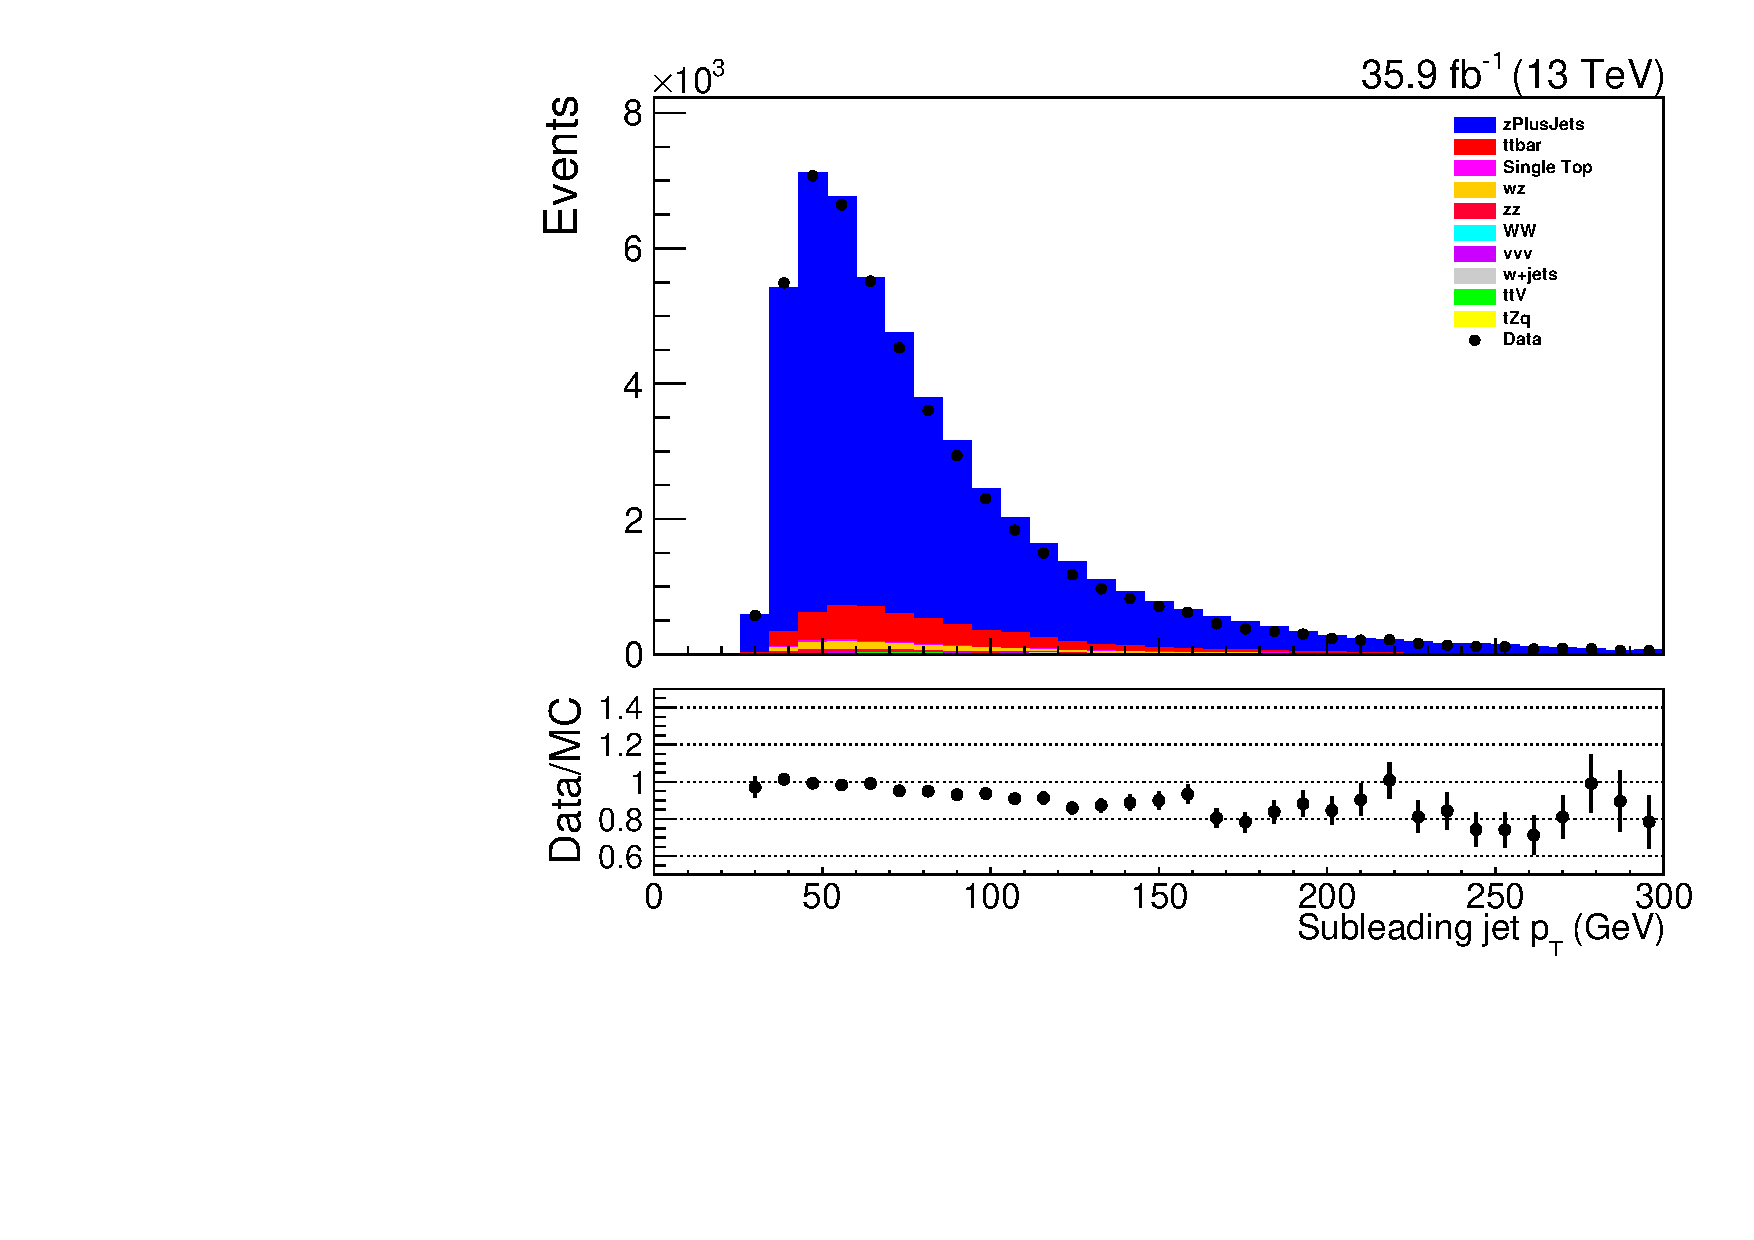
\includegraphics[width=0.47\textwidth]{figs/background-estimation/plots/unblinded/DY_control_old_prompt_ee_DYamcatnlo/secondJetPt_SingleTop_jetSel_ee.pdf}
\\
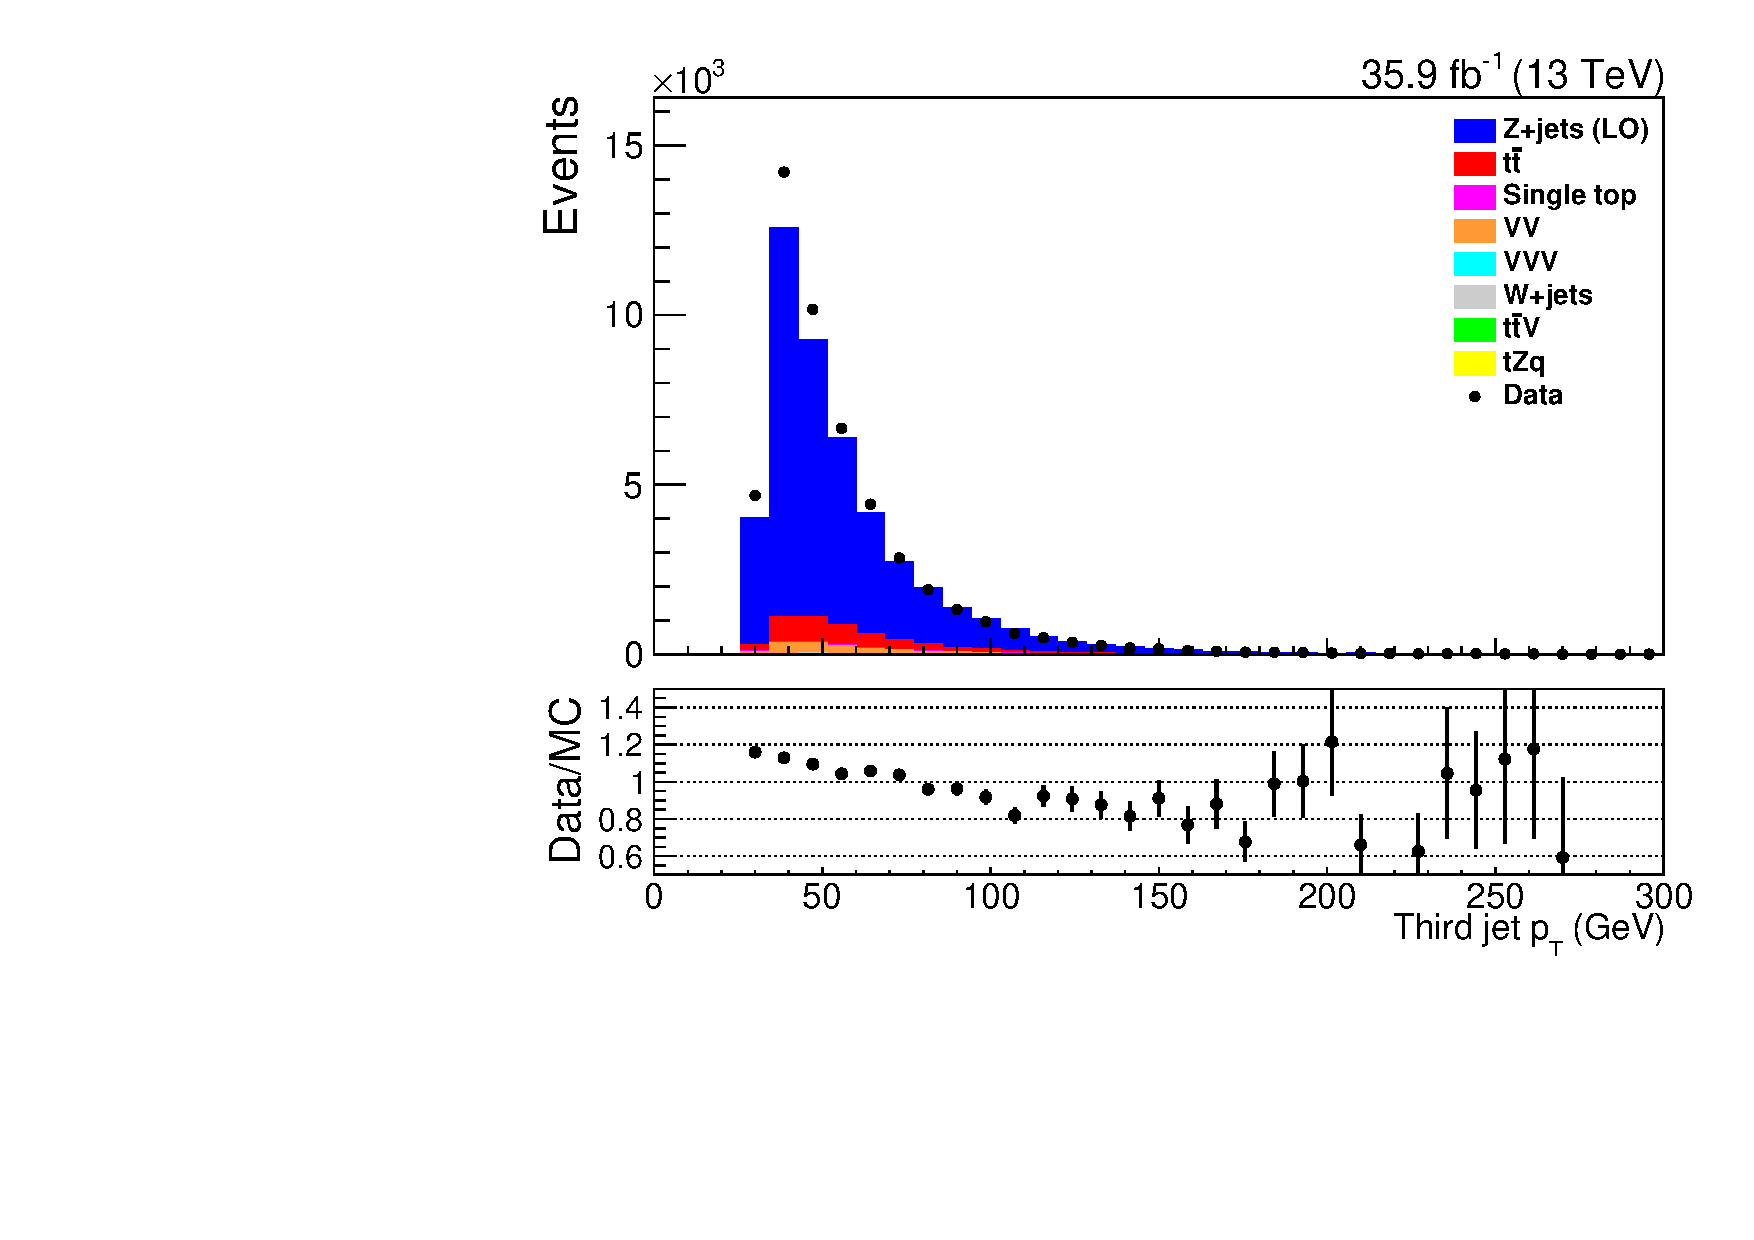
\includegraphics[width=0.47\textwidth]{figs/background-estimation/plots/unblinded/DY_control_old_prompt_ee_ttbarInc/thirdJetPt_SingleTop_jetSel_ee.pdf}
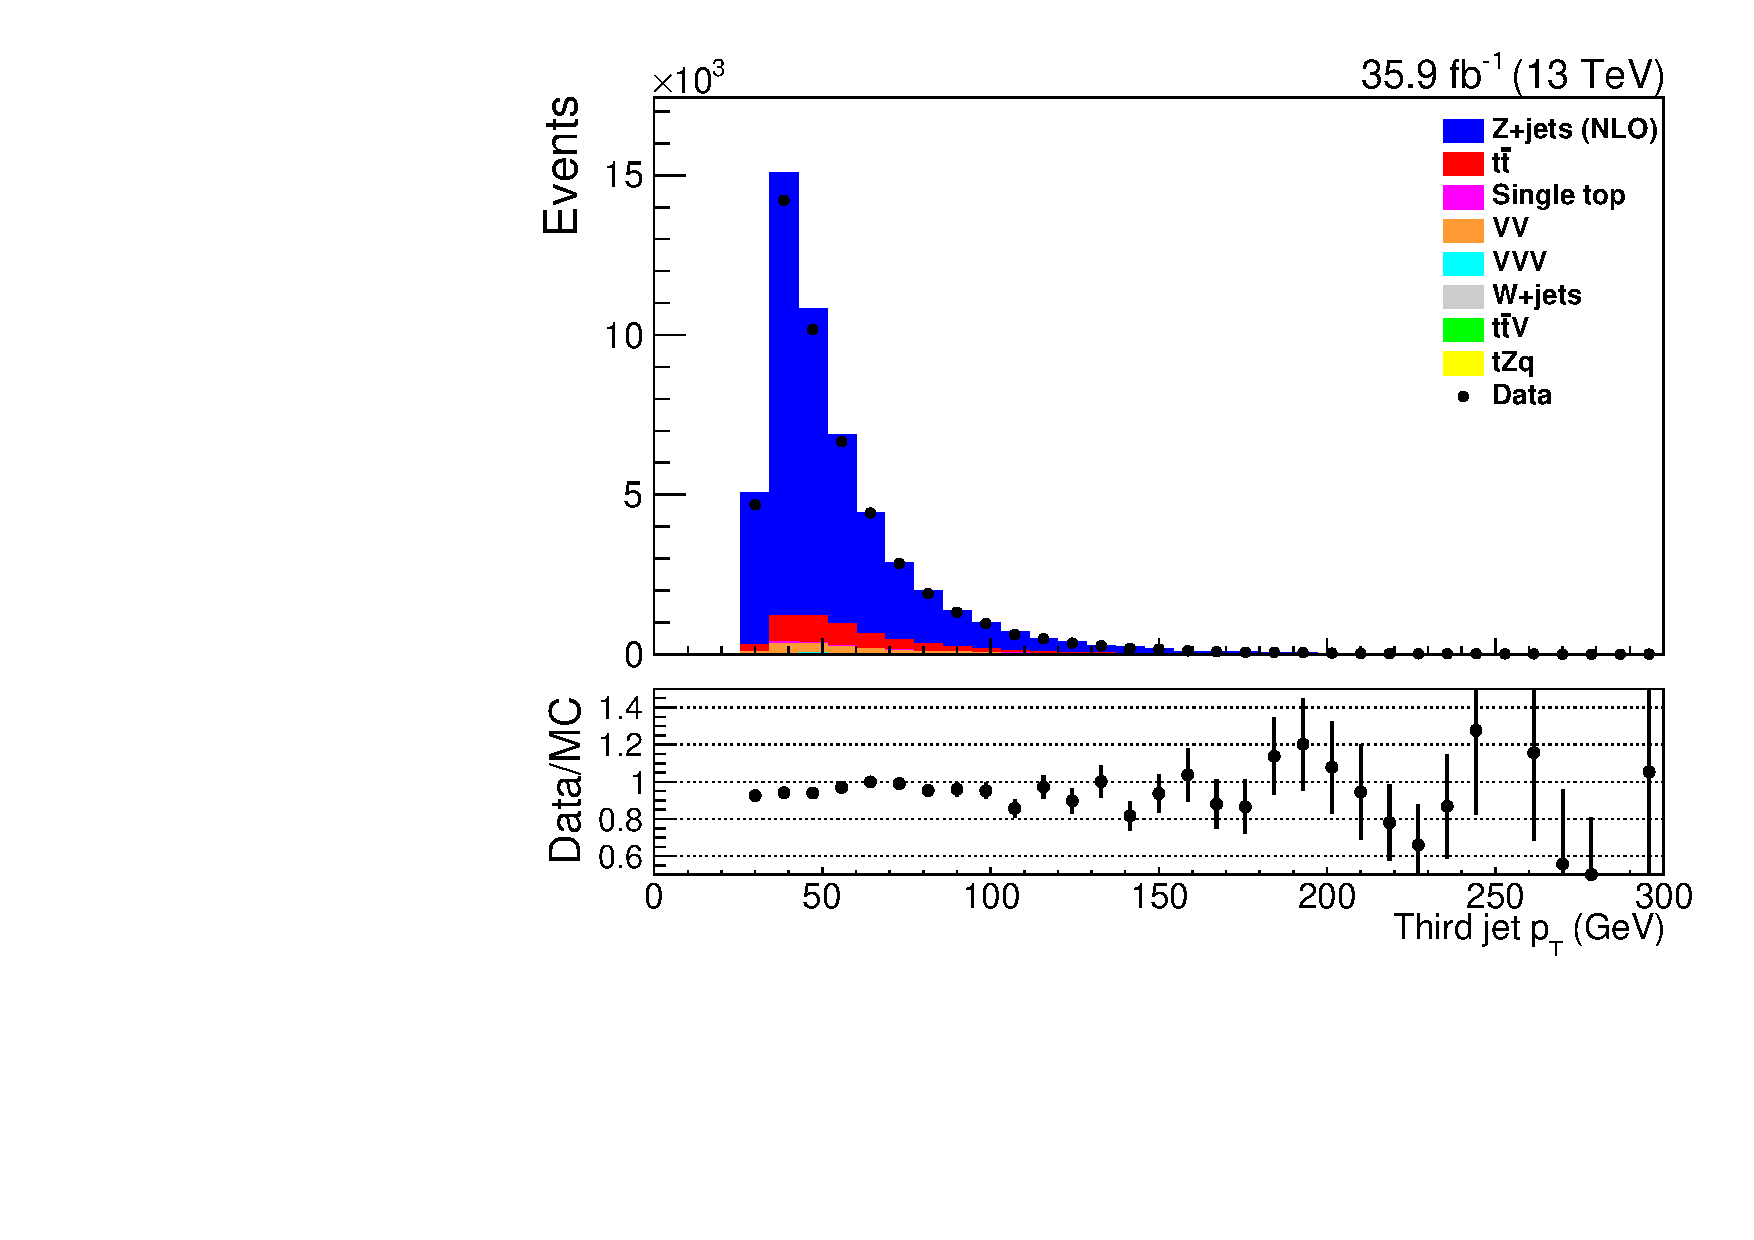
\includegraphics[width=0.47\textwidth]{figs/background-estimation/plots/unblinded/DY_control_old_prompt_ee_DYamcatnlo/thirdJetPt_SingleTop_jetSel_ee.pdf}
\\
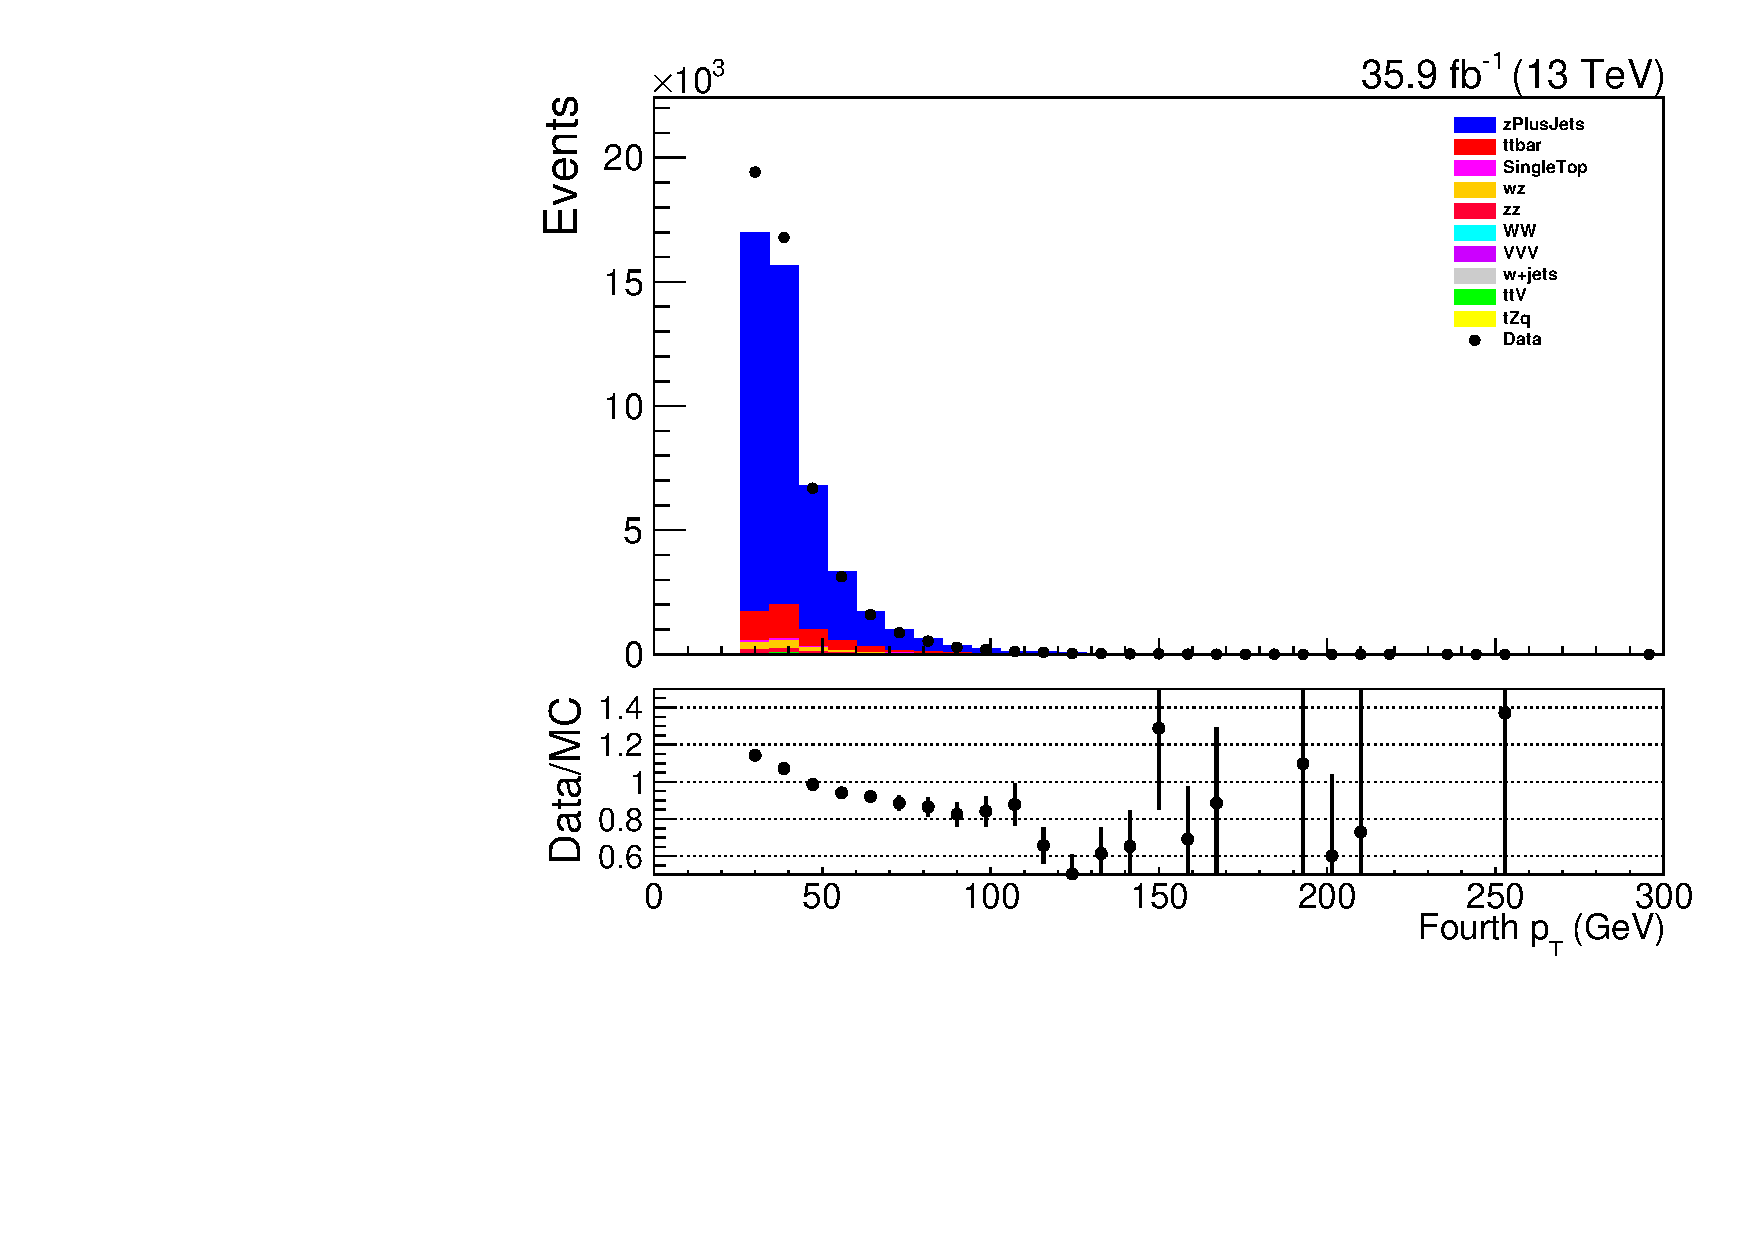
\includegraphics[width=0.47\textwidth]{figs/background-estimation/plots/unblinded/DY_control_old_prompt_ee_ttbarInc/fourthJetPt_SingleTop_jetSel_ee.pdf}
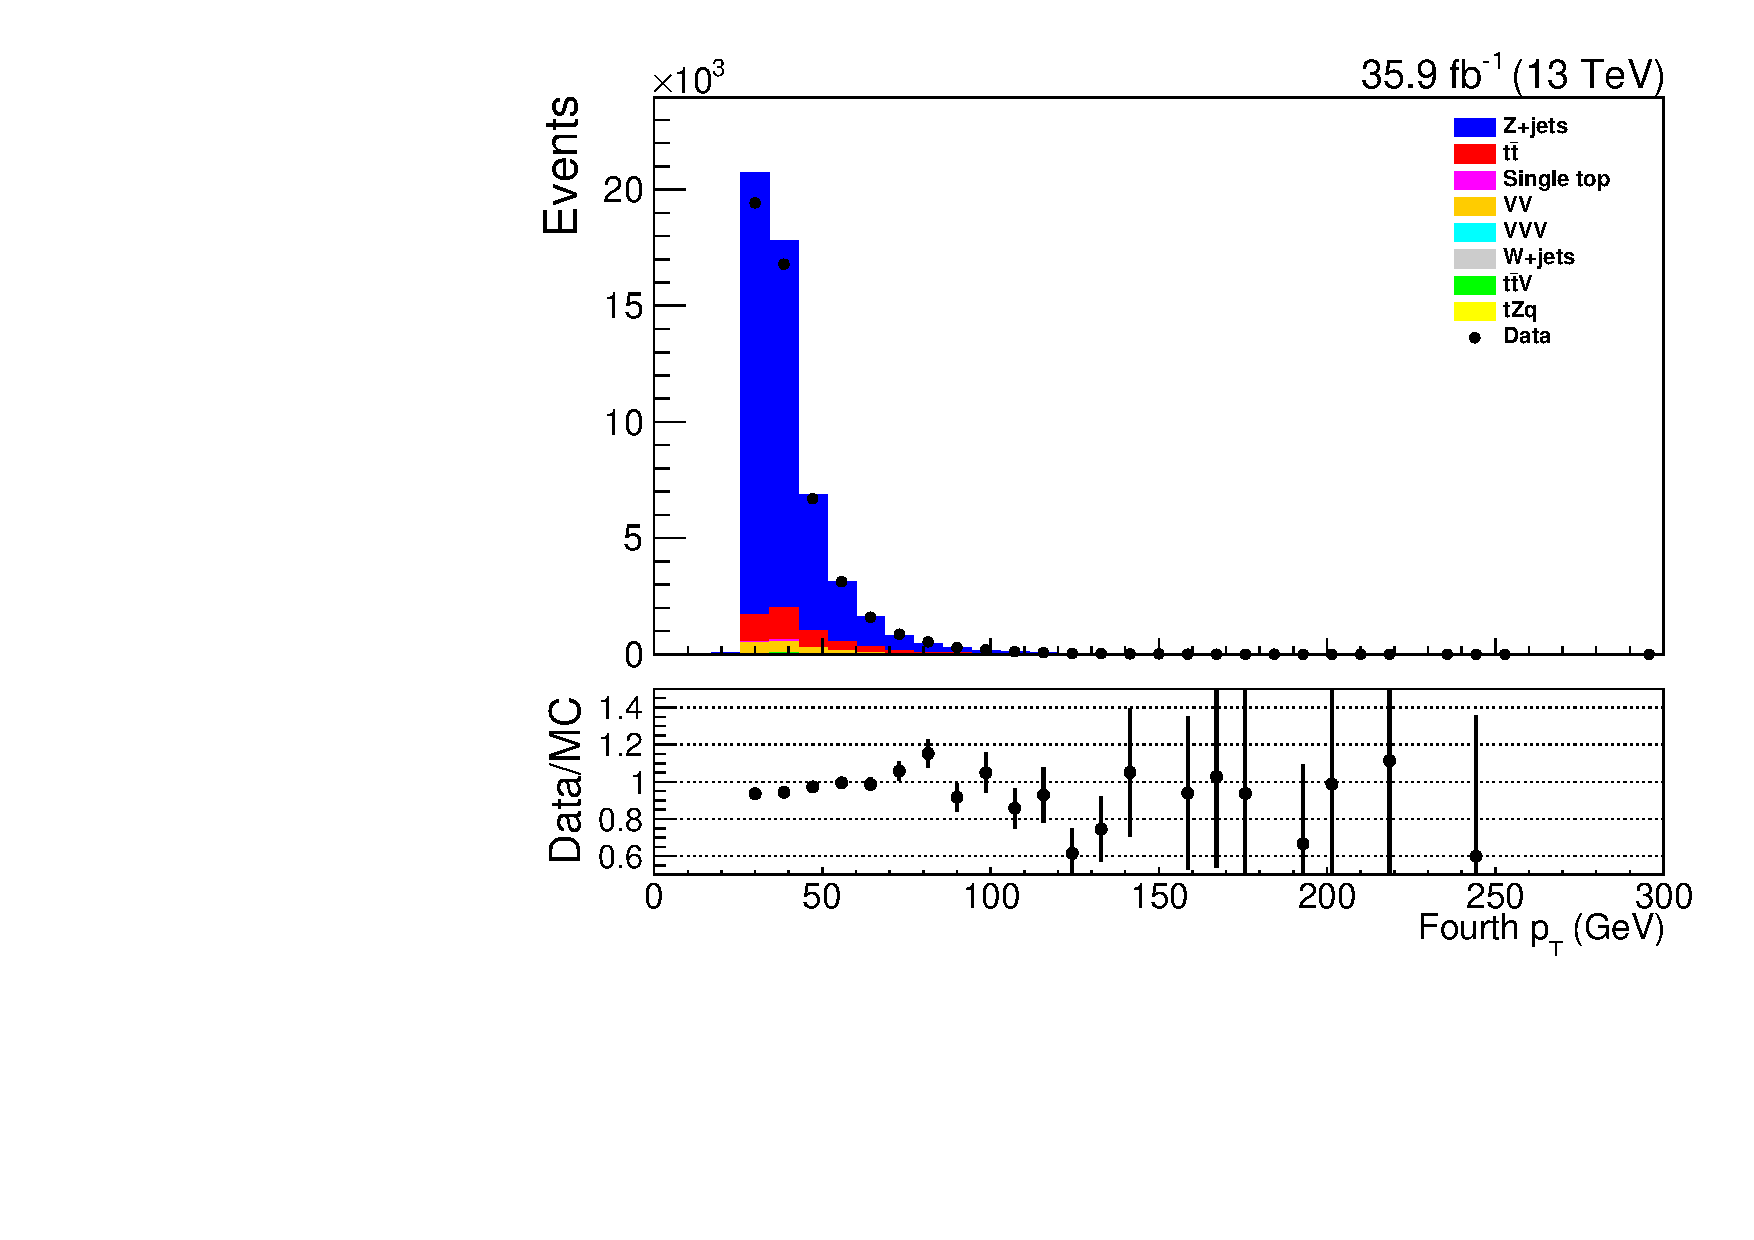
\includegraphics[width=0.47\textwidth]{figs/background-estimation/plots/unblinded/DY_control_old_prompt_ee_DYamcatnlo/fourthJetPt_SingleTop_jetSel_ee.pdf}
\caption{
The distributions of the leading four jets \pt in the 0-bjet region following the application of the jet selection criteria and simulation corrections for the LO (left) and NLO (right) Z+jets samples in the $ee$ channel.
}
\label{fig:zPlusCR_jetPt}
\end{figure}

Consequently, it was decided to use the LO Z+jets sample to model Z+jets processes despite the NLO sample providing a better description of the \pT of the higher order jets (as shown in Figure~\ref{fig:zPlusCR_jetPt}).
The reasons why the NLO Z+jets sample does not correctly normalise and poorly describes events with low jet multiplicities will need to be understood before it can be considered in the future.

\begin{table}[p]
\topcaption{The number of observed events in data and the number of expected events from simulation for the 0-bjet Z+jets control region following the application of the full event selection and simulation corrections.
These event yields are shown for each of the individual channels, as well as their combination.
}\label{tab:zPlusControlYieldsOld}
\centering
\begin{tabular}{lccccc}
\hline
Channel &  $ee$ & $\mu\mu$ & Combined \\
\hline
tZq & 20.96$\pm$0.06 & 38.47$\pm$0.08 & 59.43$\pm$0.10    \\
tWZ: & 4.38$\pm$0.18 & 7.17$\pm$0.24 & 11.55$\pm$0.30    \\
tHq: & 0.10$\pm$0.01 & 0.17$\pm$0.01 & 0.27$\pm$0.01    \\
ttW: & 2.26$\pm$0.07 & 4.90$\pm$0.12 & 7.16$\pm$0.14    \\
ttZ: & 26.05$\pm$0.14 & 43.92$\pm$0.18 & 69.97$\pm$0.23    \\
ttH: & 1.29$\pm$0.05 & 2.36$\pm$0.07 & 3.65$\pm$0.09    \\
\ttbar: & 568.32$\pm$14.67 & 1182.74$\pm$21.78 & 1751.06$\pm$26.26    \\
tW: & 30.09$\pm$2.31 & 56.88$\pm$3.22 & 86.97$\pm$3.96    \\
s-channel: & 0.0$\pm$0.0 & 0.0$\pm$0.0 & 0.0$\pm$0.0    \\
t-channel: & 0.21$\pm$0.12 & 1.48$\pm$0.32 & 1.69$\pm$0.34    \\
WW: & 14.92$\pm$1.69 & 29.21$\pm$2.43 & 44.13$\pm$2.96    \\
WZ: & 733.13$\pm$2.12 & 1282.83$\pm$2.85 & 2015.96$\pm$3.55    \\
ZZ: & 246.36$\pm$1.07 & 444.69$\pm$1.48 & 691.05$\pm$1.83    \\
WWW: & 0.69$\pm$0.15 & 1.65$\pm$0.23 & 2.34$\pm$0.27    \\
WWZ: & 10.08$\pm$0.47 & 17.17$\pm$0.63 & 27.25$\pm$0.79    \\
WZZ: & 6.19$\pm$0.22 & 9.96$\pm$0.28 & 16.15$\pm$0.36    \\
ZZZ: & 1.65$\pm$0.05 & 2.84$\pm$0.07 & 4.49$\pm$0.09    \\
W+jets: & 0.0$\pm$ & 0.0$\pm$ & 0.0$\pm$0.0    \\
\hline
Z+jets (LO): & 25102.1$\pm$180.2 & 48148.2$\pm$253.6 & 73250.3$\pm$311.10    \\
Z+jets (NLO): & 66092.6$\pm$331.5 & 125392.2$\pm$464.4 & 191484.8$\pm$570.58    \\
\hline
Total MC (LO): & 26768.8$\pm$180.8 & 51274.6$\pm$254.6 & 78043.4$\pm$312.27   \\
Total MC (NLO): & 67759.3$\pm$331.9 & 128518.6$\pm$464.9 & 196277.9$\pm$571.2    \\
\hline
Data & 27598.0$\pm$166.13 & 50814.0$\pm$255.42 & 78412.0$\pm$304.69    \\
\hline
\end{tabular}
\end{table}

\begin{table}[p]
\topcaption{The number of observed events in data and the number of expected events from simulation for the $m_{W}^{inv}$ Z+jets control region following the application of the full event selection and simulation corrections.
These event yields are shown for each of the individual channels, as well as their combination.
}\label{tab:zPlusControlYieldsNew}
\centering
\begin{tabular}{lccccc}
\hline
Channel &  $ee$ & $\mu\mu$ & Combined \\
\hline
tZq & 13.16$\pm$0.05 & 24.32$\pm$0.07 & 37.48$\pm$0.09    \\
tWZ: & 1.01$\pm$0.08 & 1.99$\pm$0.12 & 3.00$\pm$0.14    \\
tHq: & 0.05$\pm$0.01 & 0.10$\pm$0.01 & 0.15$\pm$0.01    \\
ttW: & 0.66$\pm$0.04 & 1.33$\pm$0.06 & 1.99$\pm$0.07   \\
ttZ: & 9.86$\pm$0.08 & 17.87$\pm$0.11 & 27.73$\pm$0.14    \\
ttH: & 0.52$\pm$0.03 & 1.24$\pm$0.05 & 1.76$\pm$0.06    \\
\ttbar: & 403.56$\pm$11.78 & 827.84$\pm$17.31 & 1234.40$\pm$20.94    \\
tW: & 10.83$\pm$1.31 & 25.79$\pm$2.11 & 36.62$\pm$2.48    \\
s-channel: & 0.0$\pm$0.0 & 0.0$\pm$0.0 & 0.0$\pm$0.0    \\
t-channel: & 0.22$\pm$0.10 & 0.68$\pm$0.21 & 0.90$\pm$0.23    \\
WW: & 0.18$\pm$0.10 & 0.0$\pm$0.0 & 0.18$\pm$0.10    \\
WZ: & 39.43$\pm$0.50 & 68.57$\pm$0.67 & 108.0$\pm$0.84    \\
ZZ: & 33.43$\pm$0.42 & 59.54$\pm$0.57 & 92.97$\pm$0.71    \\
WWW: & 0.0$\pm$0.0 & 0.04$\pm$0.04 & 0.04$\pm$0.04    \\
WWZ: & 0.25$\pm$0.06 & 0.78$\pm$0.13 & 1.03$\pm$0.14    \\
WZZ: & 0.48$\pm$0.06 & 0.71$\pm$0.07 & 1.19$\pm$0.09    \\
ZZZ: & 0.20$\pm$0.02 & 0.25$\pm$0.02 & 0.45$\pm$0.03    \\
W+jets: & 0.0$\pm$0.0 & 0.0$\pm$0.0 & 0.0$\pm$0.0    \\
\hline
Z+jets (LO): & 2259.5$\pm$54.5 & 4363.7$\pm$77.2 & 6623.2$\pm$94.50    \\
Z+jets (NLO): & 6922.4$\pm$107.9 & 13147.4$\pm$151.8 & 20069.8$\pm$186.24    \\
\hline
Total MC (LO): & 2773.3$\pm$55.78 & 5394.7$\pm$79.15 & 8168.0$\pm$96.83    \\
Total MC (NLO): & 7436.2$\pm$108.55 & 14178.4$\pm$152.80 & 21614.6$\pm$187.43    \\
\hline
Data: & 2940.0$\pm$64.2 & 5718.0$\pm$87.2 & 8658.0$\pm$108.28    \\
\hline
\end{tabular}
\end{table}

\newpage
\subsection{\ttbar Background}\label{subsec:ttbarEstimation}
In Section~\ref{subsec:ttbarCR} a \ttbar enriched control regions was defined to produce an orthogonal region that was topologically similar to the signal region to validate the modelling of the simulated \ttbar sample used.
This control region differed from the signal region by requiring that the event contained an electron and muon, rather than a pair of electrons or muons.

Good agreement is observed between the normalisation of simulation and data at every stage of applying the simulation corrections and control region selection criteria, as illustrated in Figure~\ref{fig:ttbar_cutFlow}.

\begin{figure}[!h]
\centering
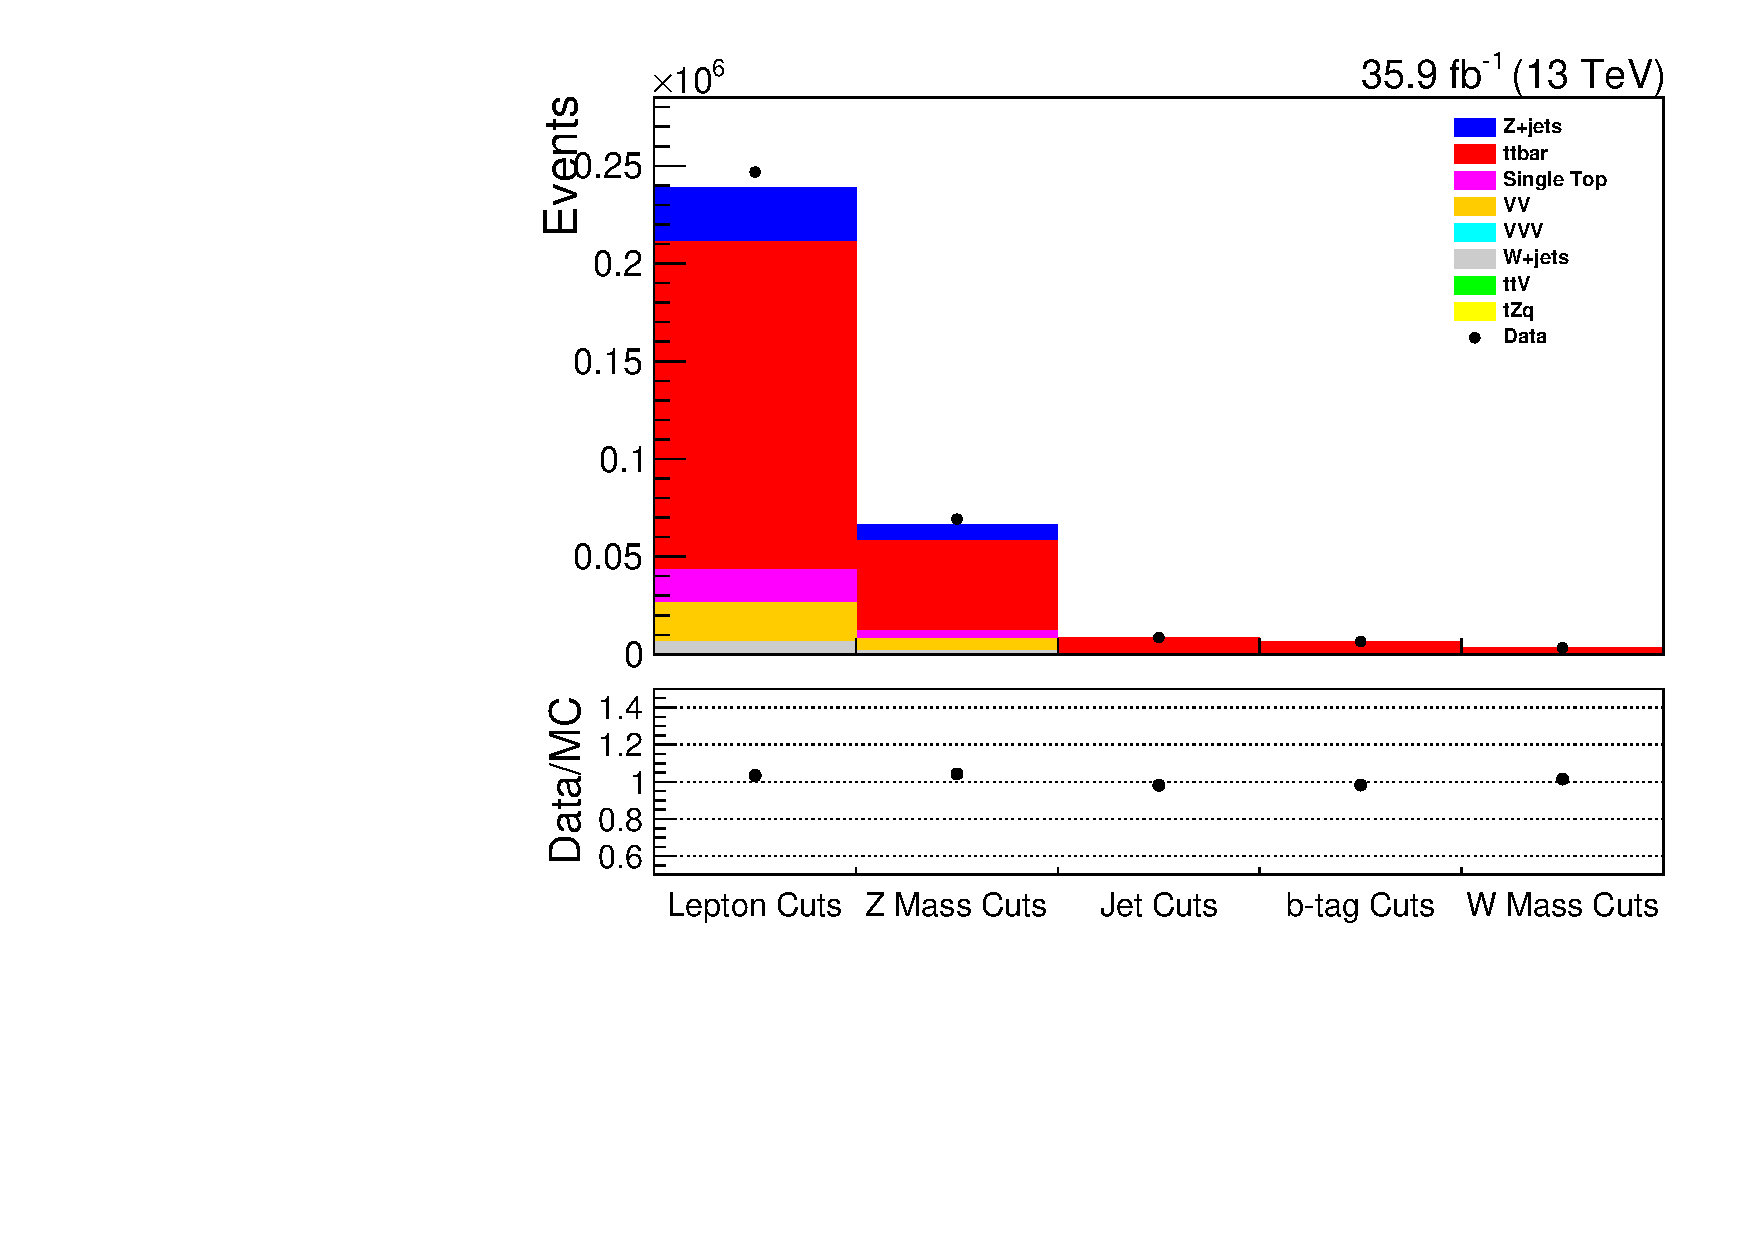
\includegraphics[width=0.6\textwidth]{figs/background-estimation/plots/unblinded/ttbar_control/cutFlow_log.pdf}
\caption{
The overall event yield for data and simulation at each stage of applying the \ttbar control region selection criteria and simulation corrections.
}
\label{fig:ttbar_cutFlow}
\end{figure}

From table~\ref{tab:ttbarCR}, it can be seen that the full application of the control region's criteria selection produces an enriched region where 97.5\% of the expected events are from \ttbar production.
Of the remaining events, 70\% are expected to be from tW single top production.

\begin{table}[h]
\topcaption {
The event yields, and the statistical uncertainties associated with them, following the full event selection and simulation corrections for the \ttbar control region.
}
\label{tab:ttbarCR}
  \centering
% This right-aligns numbers in column, but centers them under column title.
 \begin{tabular}{cc}
   \hline
   \textbf{MC process} & \textbf{$e\mu$}  \\
   \hline
	tZq\@: & 0.42$\pm$0.01  \\
	tWZ\@: & 0.14$\pm$0.03  \\
	tHq\@: & 0.32$\pm$0.01  \\
	ttW\@: & 11.90$\pm$0.15   \\
	ttZ\@: & 10.90$\pm$0.13   \\
	ttH\@: & 8.71$\pm$0.13  \\
	\ttbar: & 3288.4$\pm$31.4   \\
	tW\@: & 112.59$\pm$5.76   \\
	s-channel\@: &  0.0$\pm$0.0 \\
	t-channel\@: & 0.70$\pm$0.27 \\
	WW\@: & 1.77$\pm$0.56  \\
	WZ\@: & 0.61$\pm$0.16 \\
	ZZ\@: & 0.11$\pm$0.02 \\
	WWW\@: & 0.18$\pm$0.06     \\
	WWZ\@: & 0.09$\pm$0.05     \\
	WZZ\@: & 0.0$\pm$0.0     \\
	ZZZ\@: & 0.0$\pm$0.0     \\
	W+jets\@: & 0.0$\pm$0.0     \\
	Z+jets\@: & 0.0$\pm$0.0     \\
	\hline
	Total MC\@: & 3366.84$\pm$31.93     \\
	\hline
	Data\@: & 3396.0$\pm$58.26     \\
   \hline
 \end{tabular}
\end{table}

Good agreement is also observed for the reconstructed variables, as illustrated by the distributions of the number of jets and b-jets in Figure~\ref{fig:ttbarCR_nJets}; the \pT of the four leading jets in Figure~\ref{fig:ttbarCR_jetPt}; and the invariant mass and \pT of the two leptons in Figure~\ref{fig:ttbarCR_leptons}.

Given the good agreement observed between data and simulation, it was determined that the \ttbar MC sample accurately modelled data.
Consequently, a data-driven estimate of the \ttbar contribution was deemed unnecessary.

\begin{figure}[h]
\centering
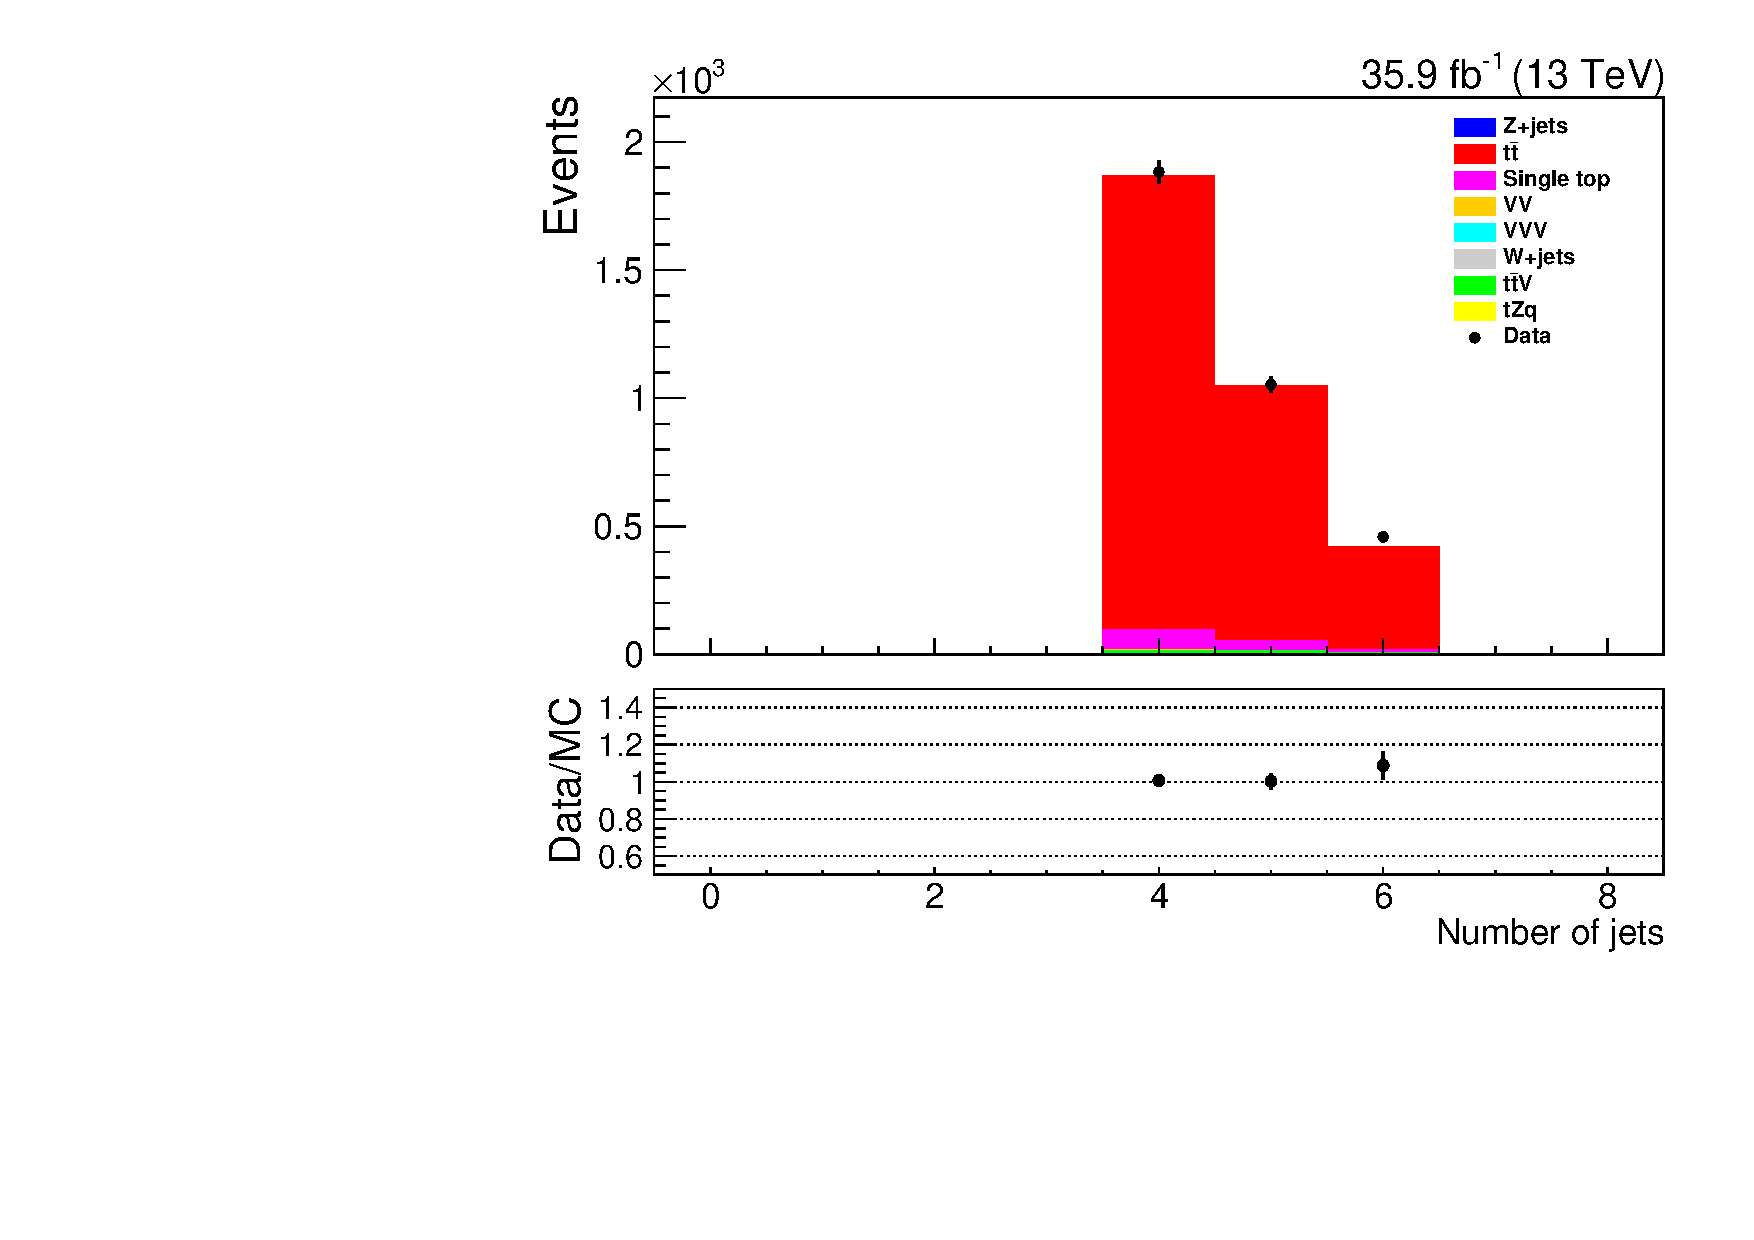
\includegraphics[width=0.47\textwidth]{figs/background-estimation/plots/unblinded/ttbar_control/numbJets_SingleTop_wMass_emu.pdf}
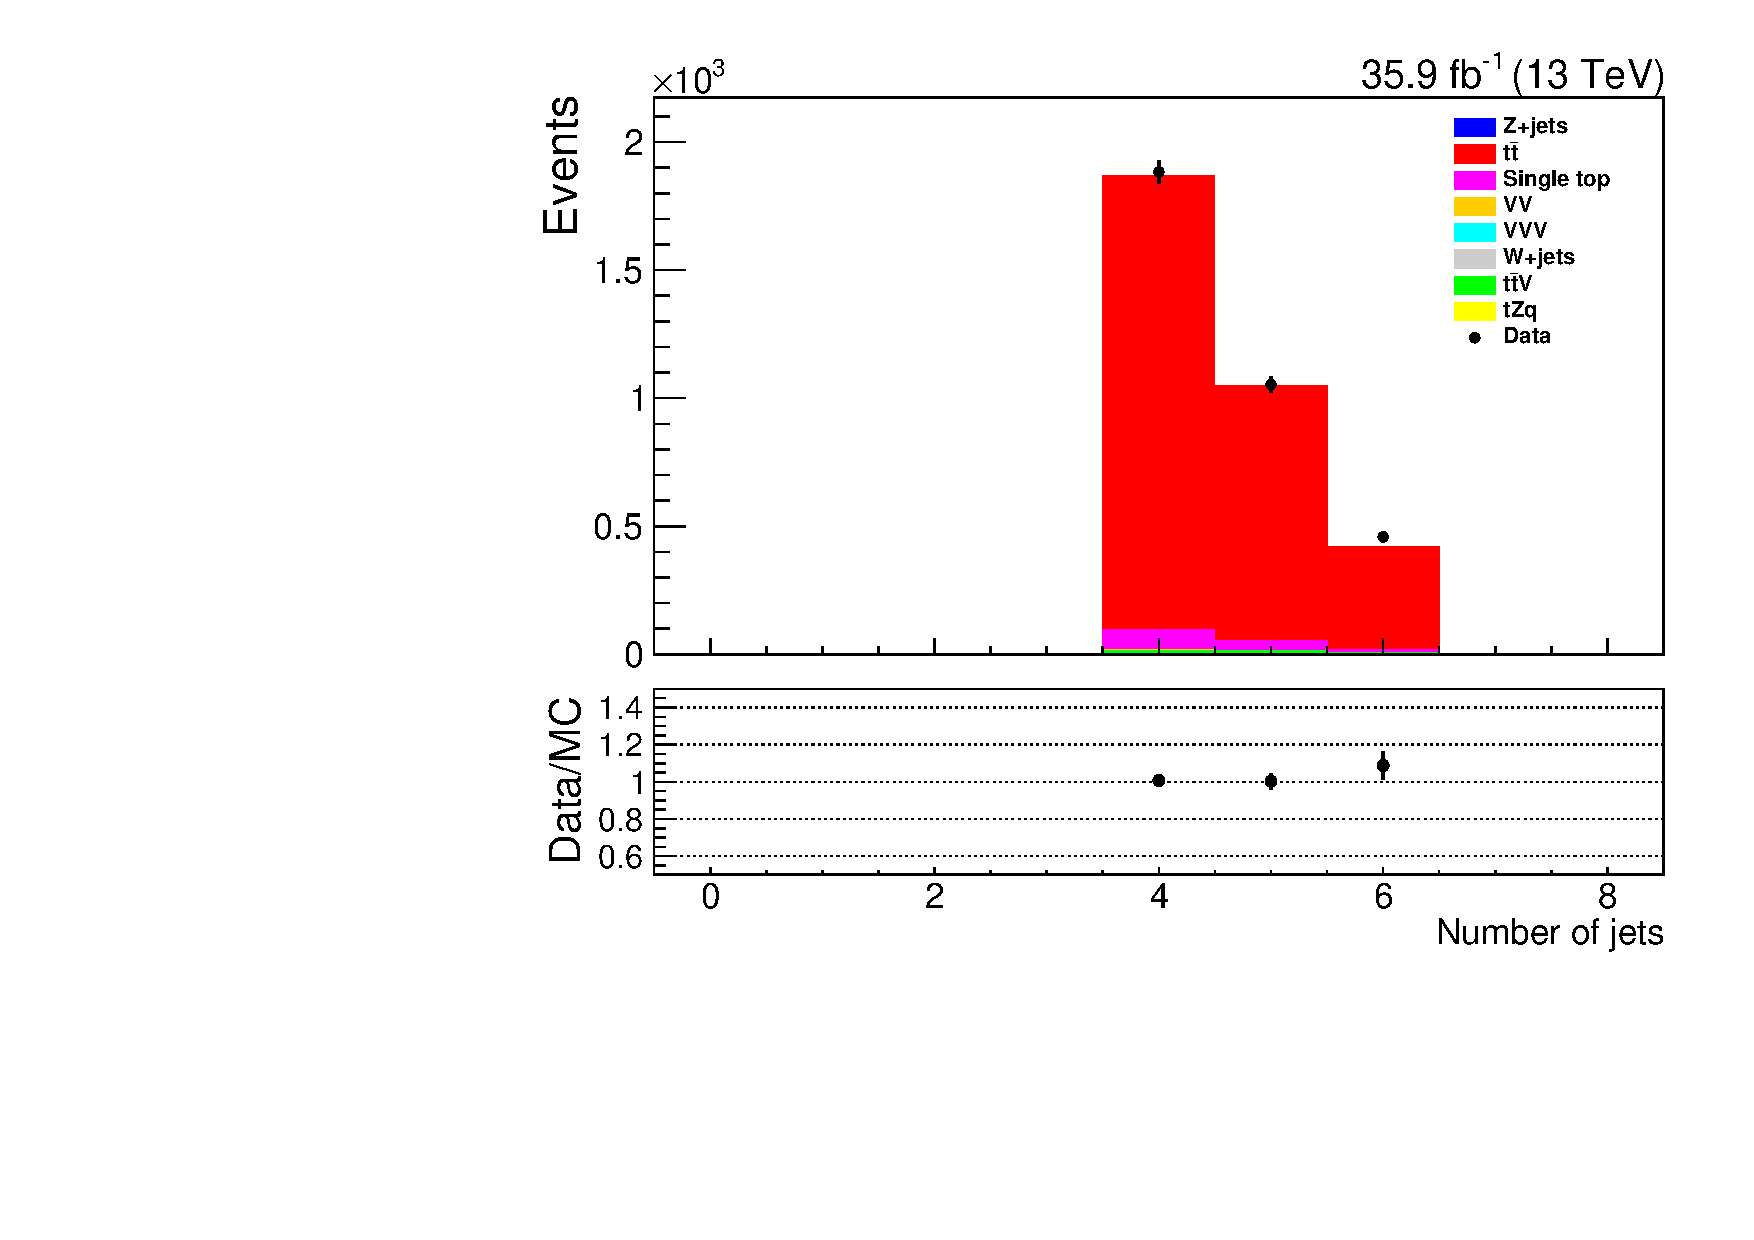
\includegraphics[width=0.47\textwidth]{figs/background-estimation/plots/unblinded/ttbar_control/numbJets_SingleTop_wMass_emu.pdf}
\caption{
The distributions of the number of jets and the number b-tagged jets for the \ttbar control region following the application of the full control region selection criteria and simulation corrections.
}
\label{fig:ttbarCR_nJets}
\end{figure}

\begin{figure}[h]
\centering
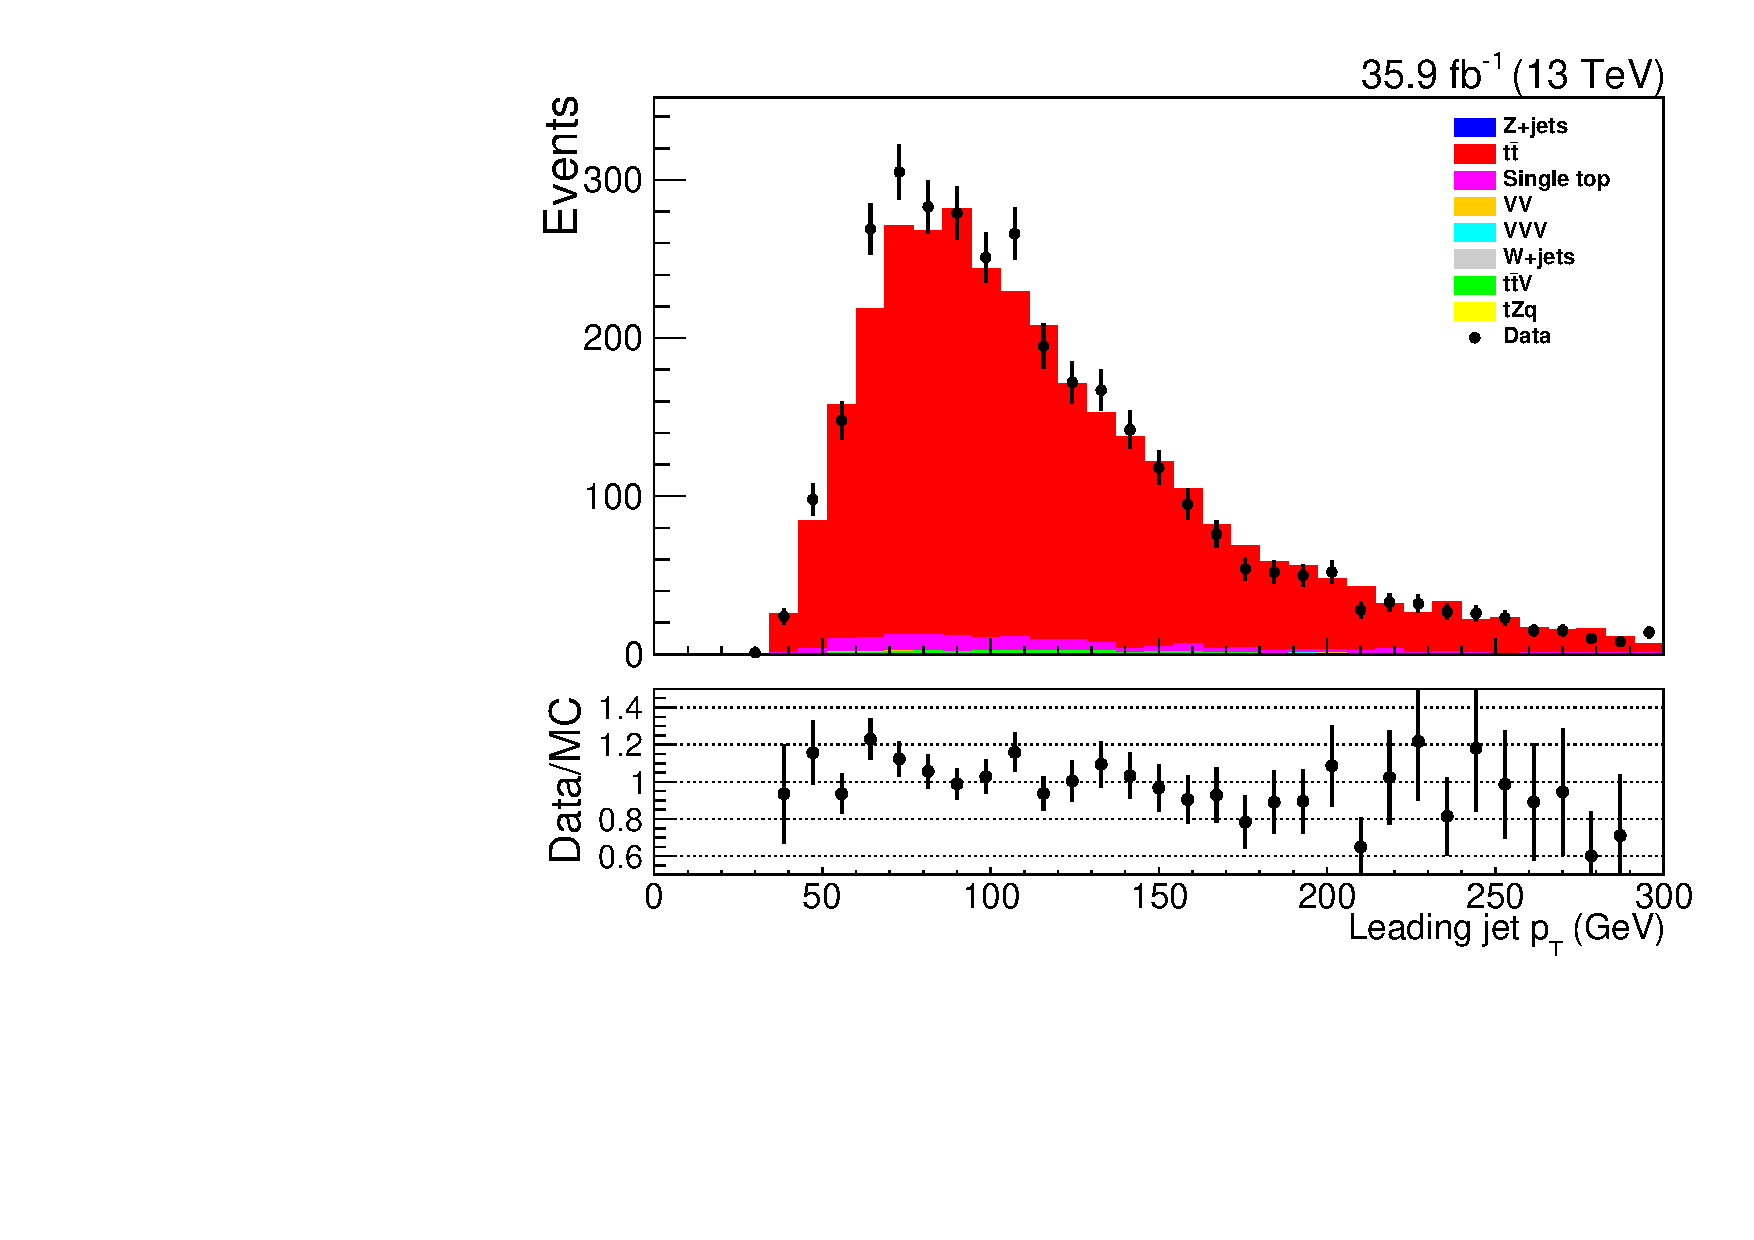
\includegraphics[width=0.47\textwidth]{figs/background-estimation/plots/unblinded/ttbar_control/leadingJetPt_SingleTop_wMass_emu.pdf}
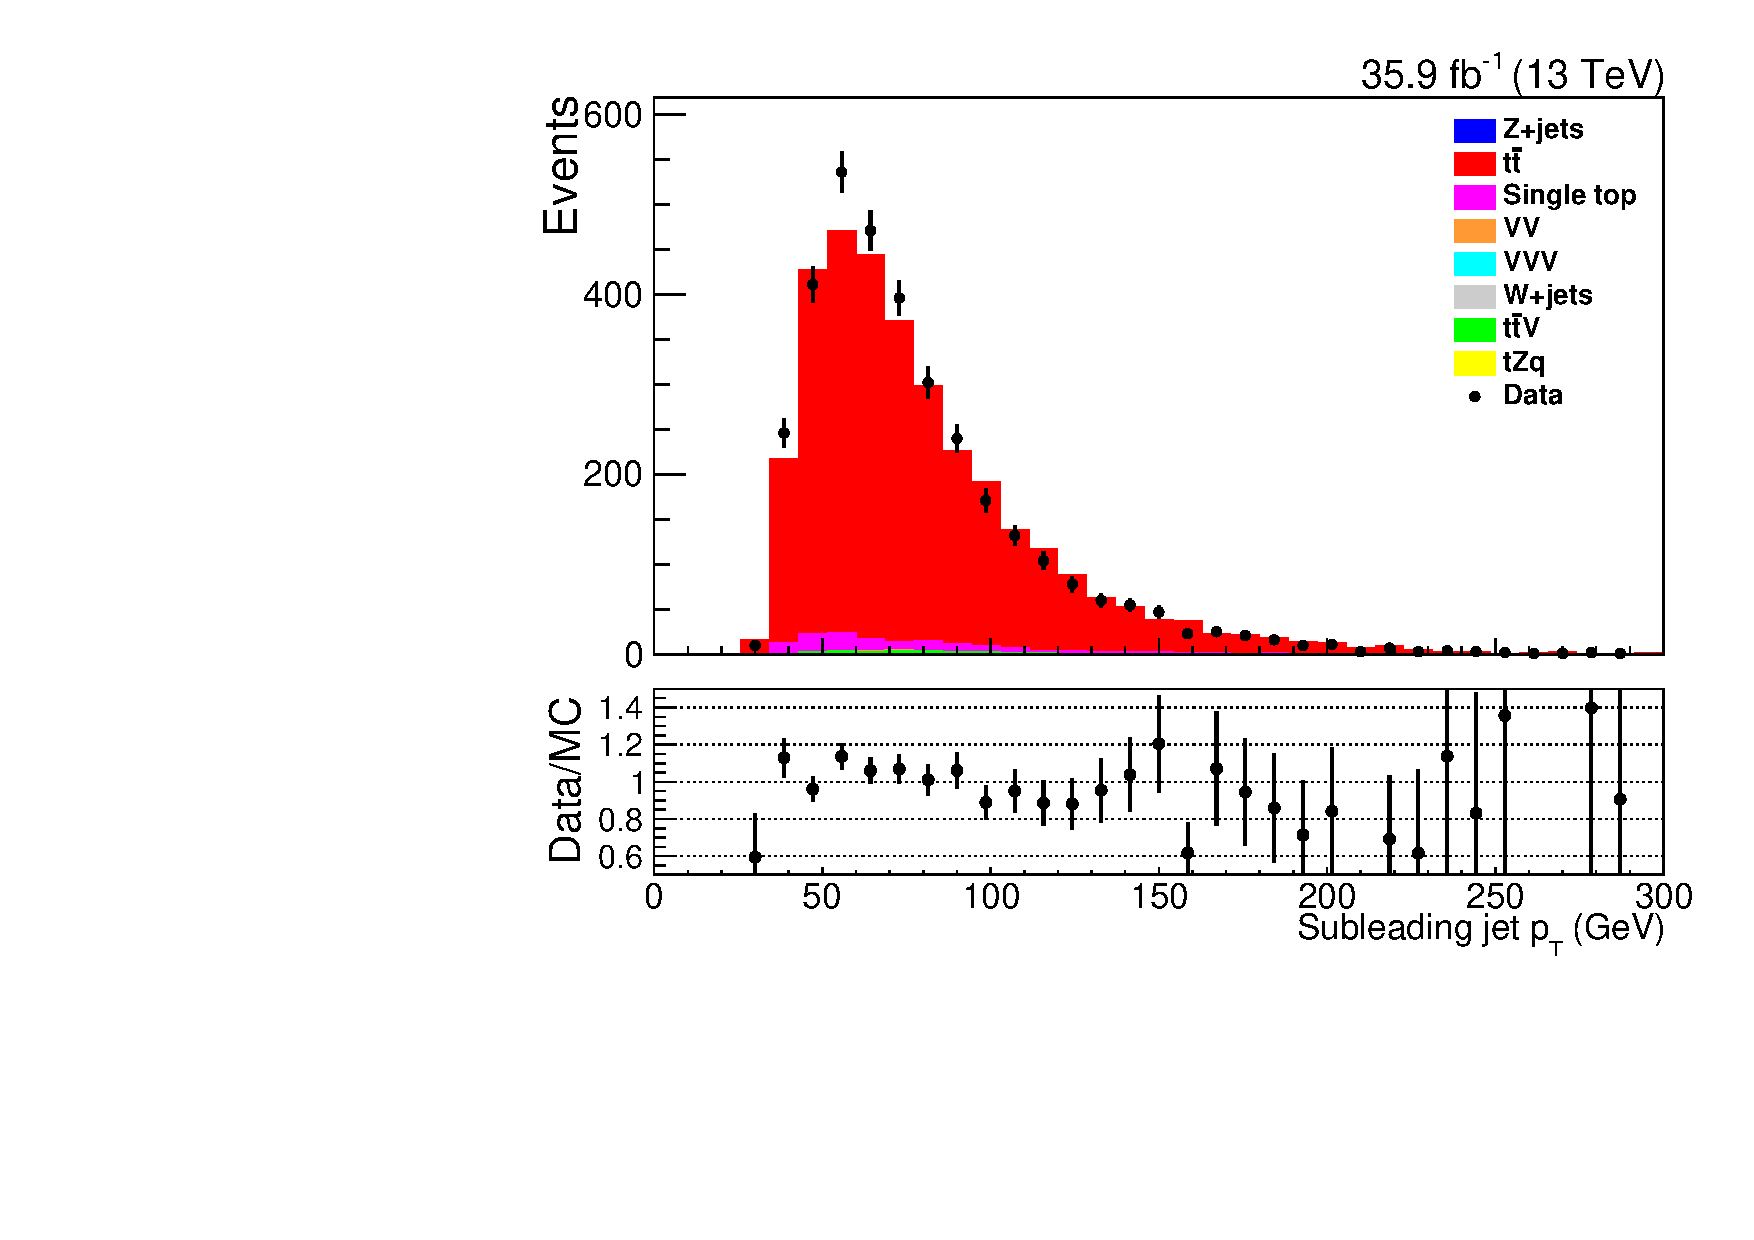
\includegraphics[width=0.47\textwidth]{figs/background-estimation/plots/unblinded/ttbar_control/secondJetPt_SingleTop_wMass_emu.pdf}
\\
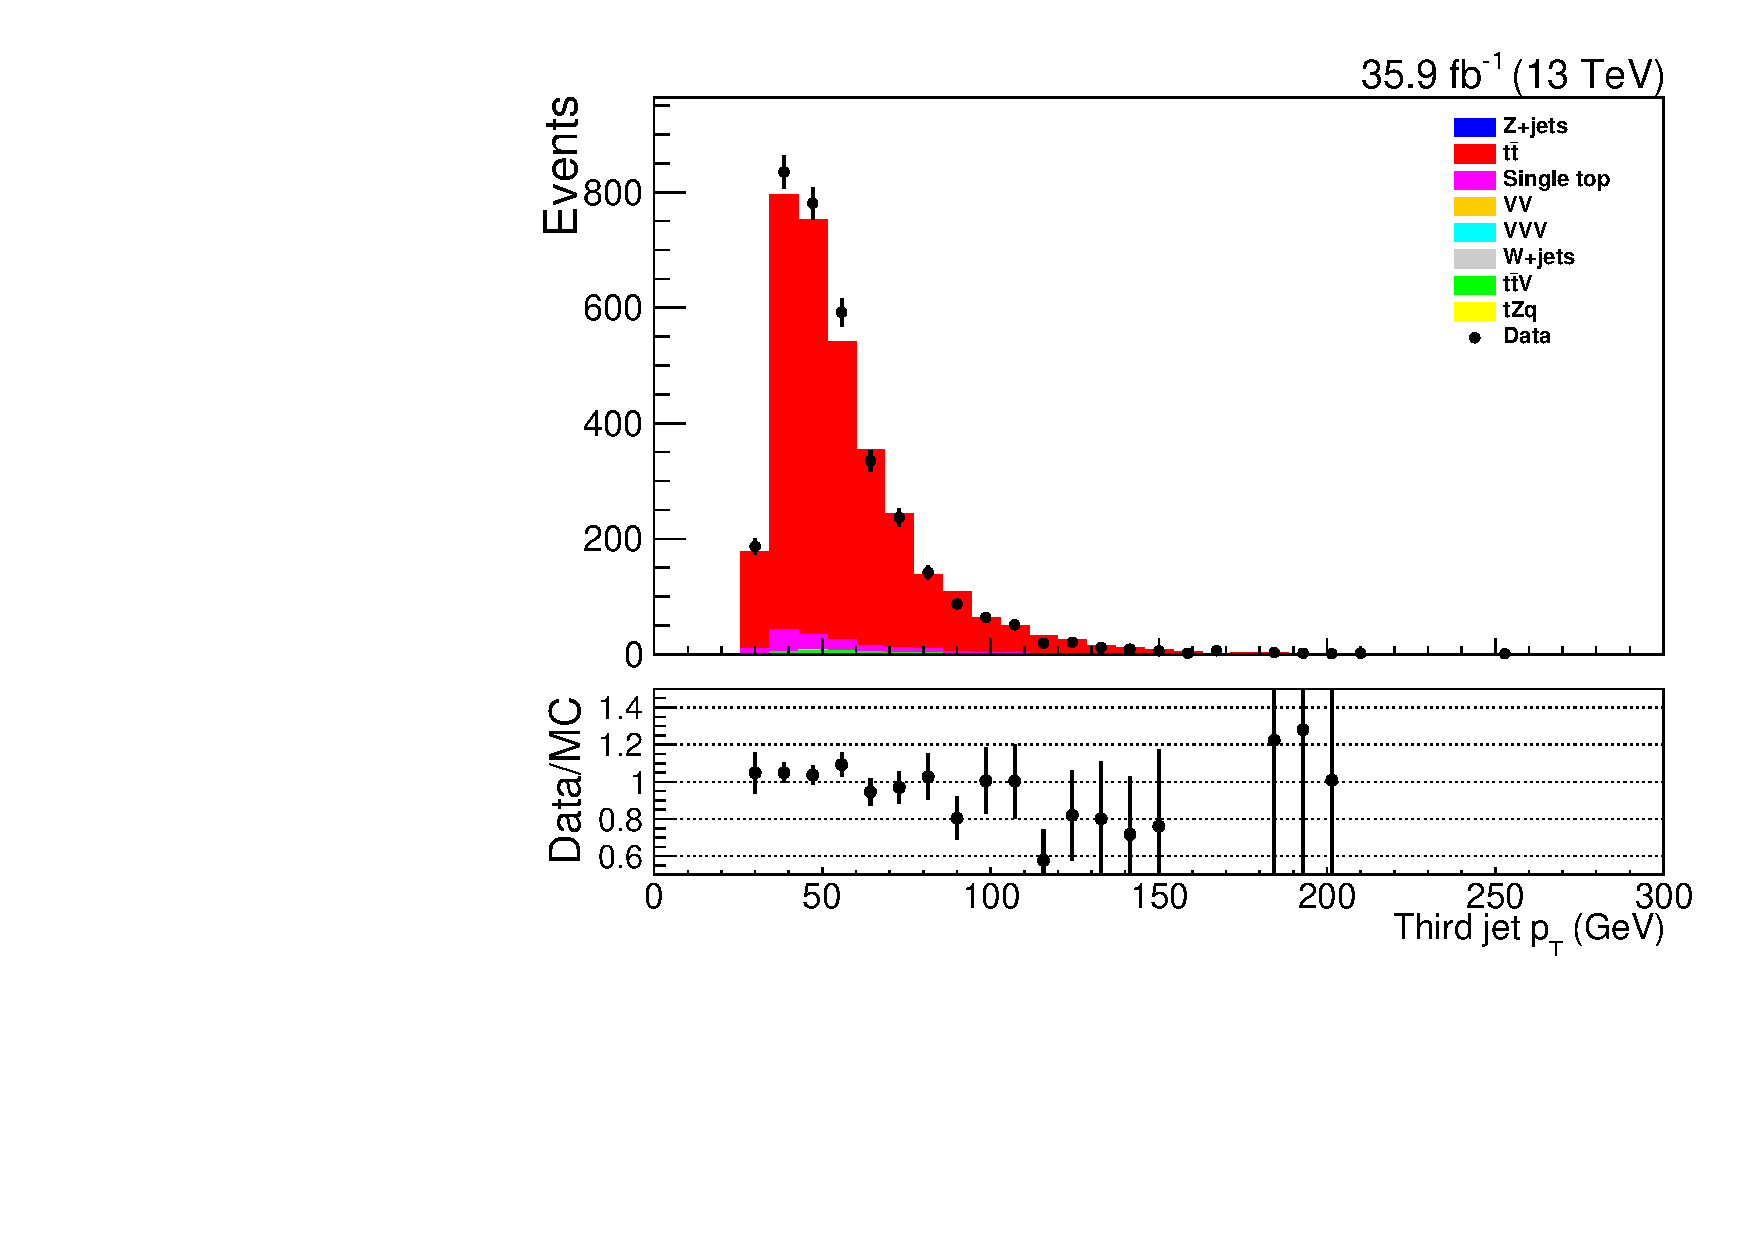
\includegraphics[width=0.47\textwidth]{figs/background-estimation/plots/unblinded/ttbar_control/thirdJetPt_SingleTop_wMass_emu.pdf}
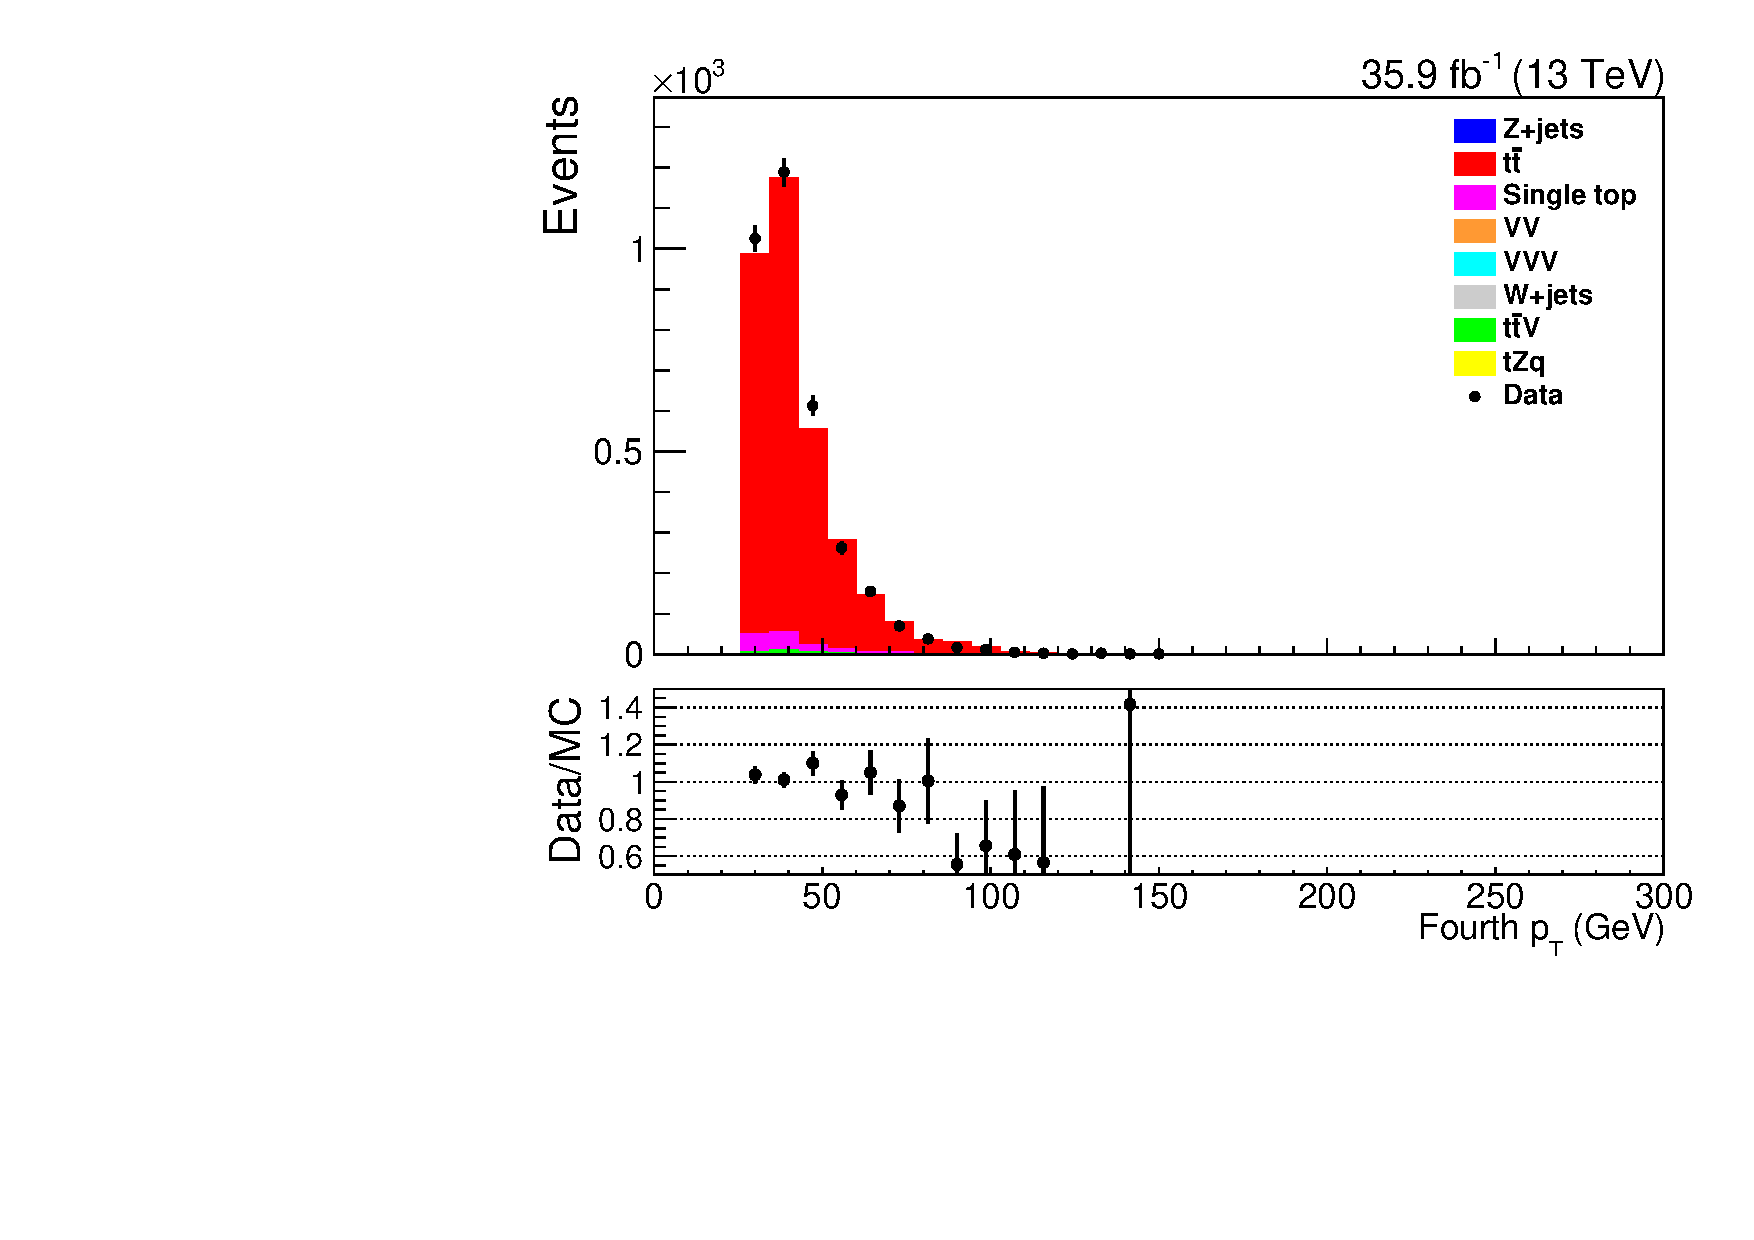
\includegraphics[width=0.47\textwidth]{figs/background-estimation/plots/unblinded/ttbar_control/fourthJetPt_SingleTop_wMass_emu.pdf}
\caption{
The distribution of the \pt of the four leading jets for the \ttbar control region following the application of the full control region selection criteria and simulation corrections.
}
\label{fig:ttbarCR_jetPt}
\end{figure}

\begin{figure}[h]
\centering
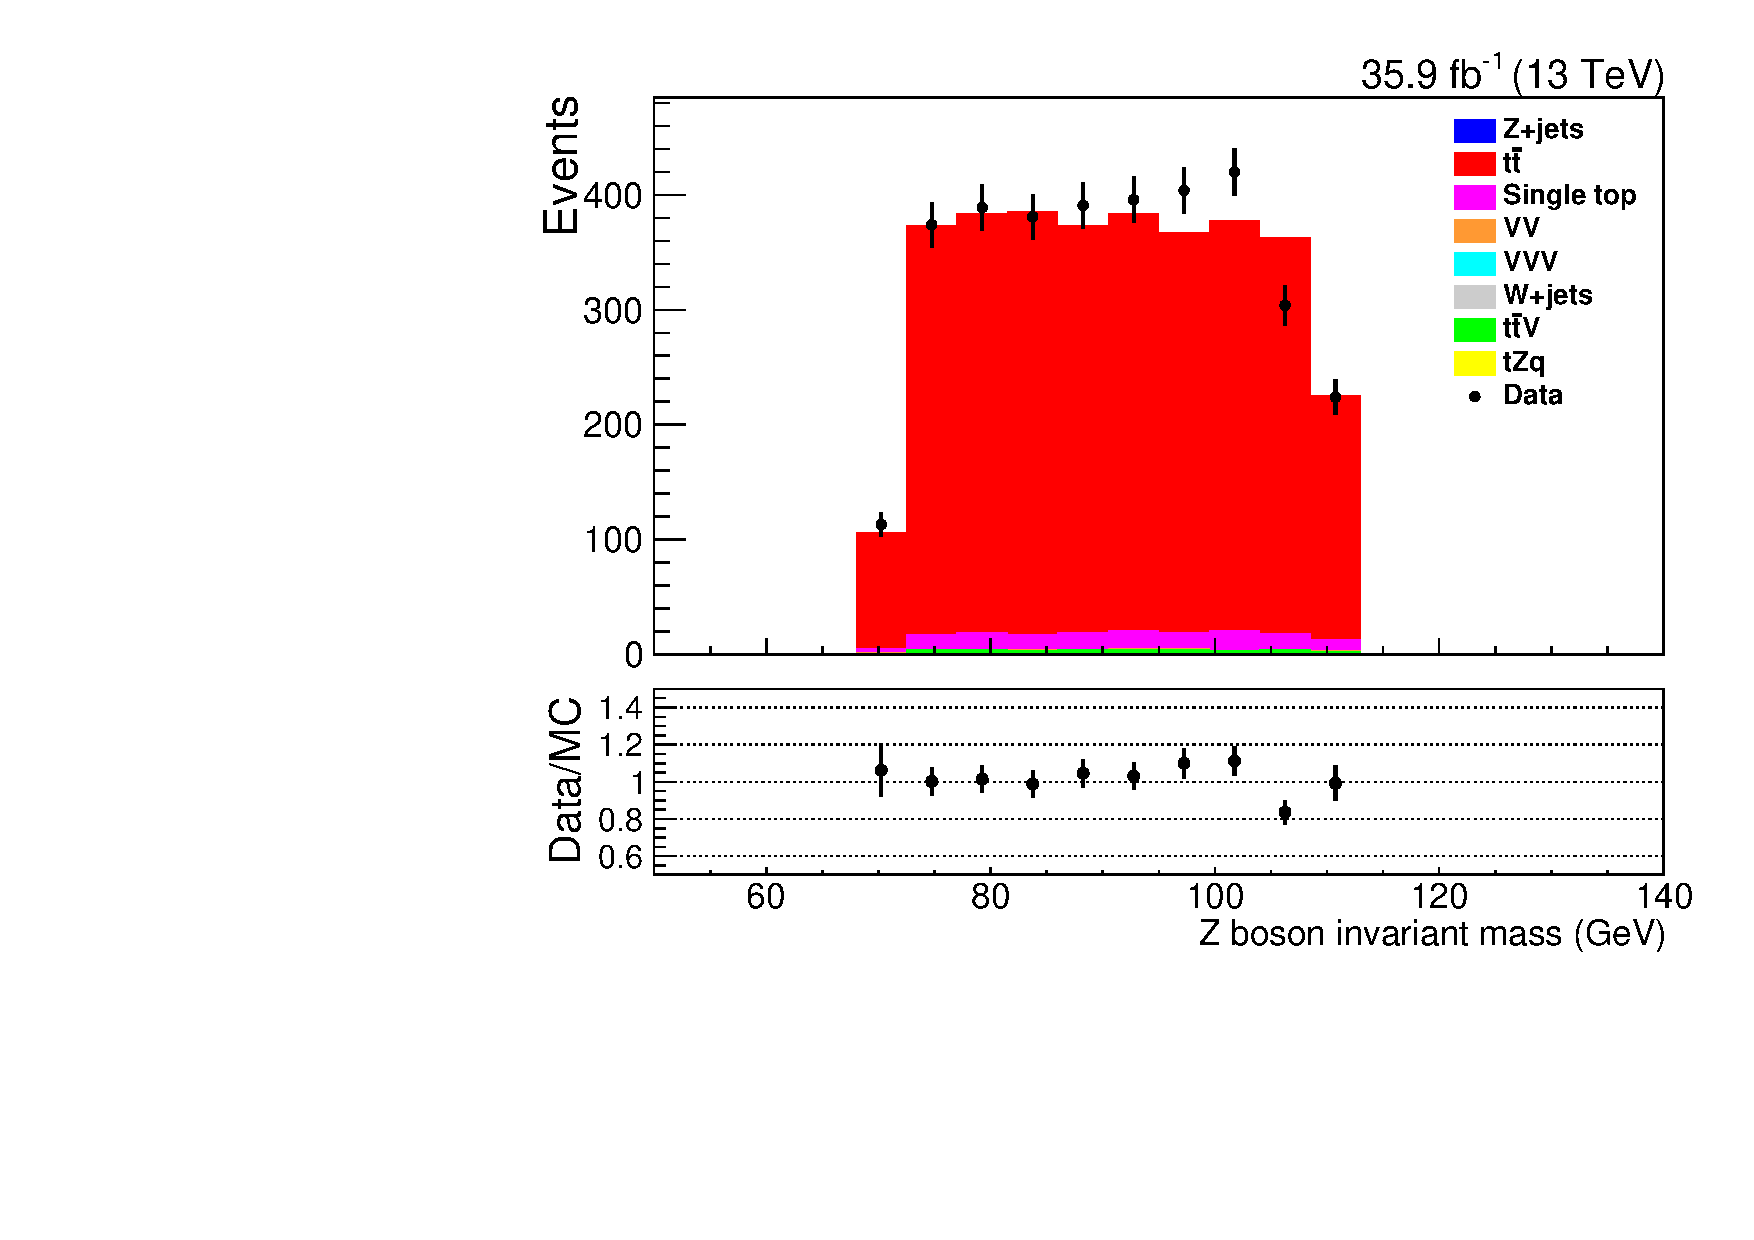
\includegraphics[width=0.49\textwidth]{figs/background-estimation/plots/unblinded/ttbar_control/zPairMass_SingleTop_wMass_emu.pdf}
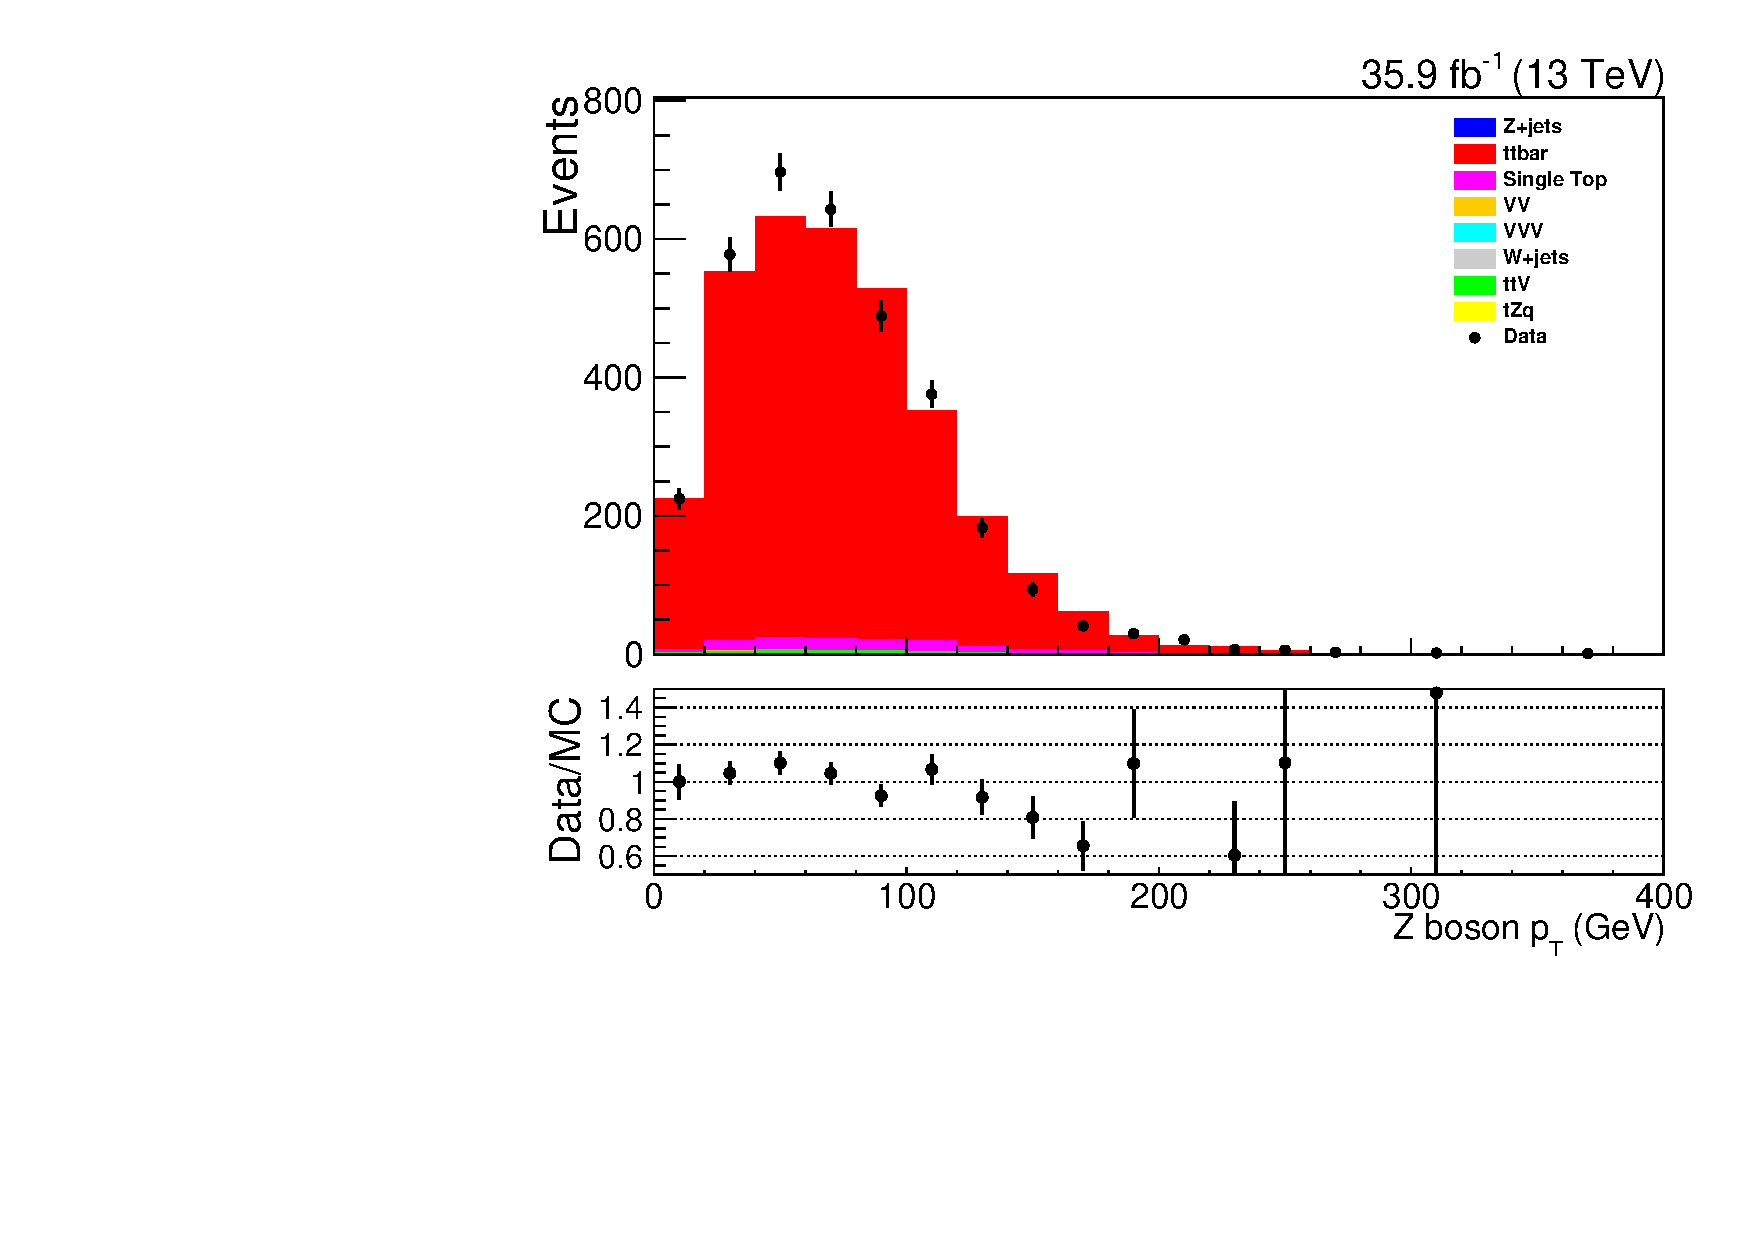
\includegraphics[width=0.49\textwidth]{figs/background-estimation/plots/unblinded/ttbar_control/zPairPt_SingleTop_wMass_emu.pdf}
\caption{
The distribution of the selected electron's and muon's combined invariant mass and \pt for the \ttbar control region following the application of the full control region selection criteria and simulation corrections.
}
\label{fig:ttbarCR_leptons}
\end{figure}

%A larger selection of data and simulation comparison plots for this control region is provided in Appendix~\ref{app:plots}.
\clearpage
\newpage
\section{Systematic Uncertainties}\label{sec:systematics}
%%% Intro
For any meaningful and robust measurement to be made in any physics analysis, it is vital that the sources of systematic uncertainties associated with it are both understood and controlled.
This is particularly important for this analysis as the low signal process production cross section compared to those of the backgrounds result in the scale of the statistical uncertainties being comparable to that of the systematic uncertainties of the measurement.

These sources of uncertainty originate from either experimental or theoretical uncertainties and influence the normalisation of the distributions considered and/or the shape of the distributions.
The statistical uncertainties arising from the size of the simulated samples available are also considered.

These uncertainties are treated as nuisance parameters in the signal extraction, which is described, along with the impact of the uncertainties on the result, in Section~\ref{sec:statisticalModel}.

\subsection{Experimental Uncertainties}
\subsubsection*{Jet Energy Corrections}
The CMS Jet Energy Corrections group provides the uncertainties associated with the JES and JER values they determine (discussed in Sections~\ref{subsubsec:JECs} and~\ref{subsec:jesjer})~\cite{Khachatryan:2016kdb}. 

The impact of the JES is evaluated by varying the JES values applied to all jets up and down by a standard deviation.
The uncertainty associated with the JER smearing is accounted for by varying the smearing factor up and down by the associated statistical uncertainty.

\subsubsection*{Missing Transverse Energy Uncertainties}
As missing transverse energy is calculated from the sum of the \pT of all PF objects in a given event along with the remaining unclustered energy deposits, the uncertainties associated with both have to be considered.

The impact of the uncertainties associated with both the JES and JER on the PF \MET are accounted for by propagating the JEC uncertainties through to the \MET and evaluating the impact they have.
As the unclustered energy remains uncorrected, the impact on the \MET uncertainty is evaluated by varying the contributions to the unclustered energy from each particle by their respective resolution.

\subsubsection*{Pileup Reweighting}
The uncertainty associated with the \PU reweighting (see Section~\ref{subsec:puSF}) is determined by varying the expected minimum bias cross section in simulation by $\pm 4.6\%$.

\subsubsection*{Parton Density Functions}\label{subsec:pdfSysts}
%%Discussion of what PDFs are, is given in an earlier chapter 
As PDFs are derived from data measured by different experiments, the uncertainties associated with each measurement must be propagated to the momentum fractions and energies that have been assigned to partons of the incoming protons.

The impact of the PDF uncertainties are evaluated according to PDF4LHC recommendations~\cite{Butterworth:2015oua}, namely as the standard deviation of the weights of the nominal and the variations of the PDF set.
For almost all of the MC samples considered, this is achieved by considering the nominal event weight and one hundred alternative PDF weights.

The single top tW-channel samples are the exception to this as at the time of their generation it was not possible to generate the required per-event weights.
In this case, the LHAPDF (Les Houches Accord Parton Distribution Function) library was used to access 100 eigenvalues from the NNPDF3.0 PDF set~\cite{Ball:2014uwa} in order to produce 200 alternative weights for each event.

\subsubsection*{b-tagging Uncertainties}
The uncertainties associated with the b-tagging scale factors described in Section~\ref{subsec:btagEff} are obtained by varying their value by $\pm 1\sigma$.

\subsubsection*{Non-prompt Lepton Contributions}
Based on the experience of other analyses which determine similar background contributions, CMS recommends a 30\% normalisation uncertainty to conservatively cover the uncertainties related to the variation of the ratio of opposite-sign over same-sign events as a function of the lepton flavour and the cut level. 
%\subsubsection*{Z+jets Background}
%The uncertainty associated with the normalisation of the aMC@NLO Z+jets background sample is evaluated as part of the signal extraction process described in Section~\ref{sec:statisticalModel}.
%This involves a simultaneous fit of the Z+jets background enriched control region and the signal region to measure the yields for both tZq and Z+jets processes.
%As such, it incorporates the impact of the statistical uncertainty on the fit of the Z+jets control region as a nuisance parameter, which then controls the normalisation of the Z+jets contribution in the final signal region fit.

\subsubsection*{Luminosity Uncertainties}
The overall uncertainty in the integrated luminosity collected by CMS in 2016 was estimated to be 2.5\%~\cite{CMS:2017_lumi}.

\subsubsection*{Lepton Efficiencies}
The uncertainties associated with the lepton identification, isolation and reconstruction efficiency scale factors discussed in Section~\ref{subsec:leptonRecoSFs} are varied by $\pm 1 \sigma$.

Several systematic studies were performed to estimate the systematic uncertainty associated with the trigger scale factors.
These studies were the comparison of the trigger efficiencies \ttbar and Z+jets processes in simulation and the strength of the correlation of the \MET trigger selection to the lepton triggers used in the analysis.

When comparing the trigger efficiencies in simulation between the for the \ttbar and Z+jets samples, it was found that the differences between the trigger efficiencies in each channel was covered by the statistical uncertainties.
The trigger efficiencies determined for the \ttbar and Z+jets simulation samples in each channel are shown in table~\ref{tab:zPlusTriggerSFs}.

\begin{table}[htbp]
\topcaption {
The trigger efficiencies for the lepton selection criteria for \ttbar and Z+jets in simulation.
The uncertainties given only include the statistical uncertainty associated with each value. 
}\label{tab:zPlusTriggerSFs}
  \centering
%  \resizebox{\textwidth}{!}{
% This right-aligns numbers in column, but centers them under column title.
 \begin{tabular}{llc}
   \hline
   \textbf{Channel} & \textbf{MC Sample} & \textbf{$\epsilon _{MC}$} \\
   \hline   
   \multirow{2}{*}{$ee$} & \ttbar & 0.98823 $\pm$ 0.00086 \\
   & Z+jets & 0.98849 $\pm$ 0.00106 \\
   \multirow{2}{*}{$\mu\mu$} & \ttbar & 0.99192 $\pm$ 0.00074 \\
   & Z+jets & 0.99258 $\pm$ 0.00083 \\
   \multirow{2}{*}{$e \mu$} & \ttbar & 0.99148 $\pm$ 0.00722 \\
   & Z+jets & 0.98838 $\pm$ 0.01183 \\
   \hline
 \end{tabular}%}
\end{table}

In order to evaluate the independence of the \MET and lepton triggers used, the efficiency of each set of triggers is first considered individually.
If both sets triggers are independent, then the efficiency of fulfilling both trigger selections can be expressed as:

\begin{equation}
\frac{\epsilon_{X + lepton triggers}}{\epsilon_{X triggers} \times \epsilon_{lepton triggers}} = \alpha
\label{eq:triggerCorrelation}
\end{equation}

If the \MET and lepton trigger selection requirements are uncorrelated, then the ratio ($\alpha$) of the left and right hand sides of equation~\ref{eq:triggerCorrelation} will be 1.
Table~\ref{tab:triggerCorrelation} shows that for the all channels, $\alpha$ only exhibits small differences from unity, indicating negligible correlation between the triggers used.

\begin{table}[htbp]
\topcaption {
The values of $\alpha$, expressing the strength of correlation between the lepton and cross triggers used to determine the trigger scale factors, for each channel.
}\label{tab:triggerCorrelation}
  \centering
%  \resizebox{\textwidth}{!}{
% This right-aligns numbers in column, but centers them under column title.
 \begin{tabular}{cc}
   \hline
   \textbf{Channel} & \textbf{$\alpha$}   \\
   \hline   
   $ee$ & 0.99890 $\pm$ 0.01379\\
   $\mu\mu$ & 1.00151 $\pm$ 0.01291\\
   $e \mu$ & 0.98883 $\pm$ 0.09415\\
   \hline
 \end{tabular}%}
\end{table}

Both the statistical uncertainties of the trigger efficiencies and the results of the above studies were consistent with those determined for other top physics analyses.
As such, it was determined that systematic uncertainties of 1.0\%, 1.0\% and 2.0\% for the $ee$, $\mu\mu$, and $e\mu$ channels, respectively, would be sufficient to account for the residual differences in trigger efficiency between data and simulation.

%The impact on the scale factors of applying the analysis selection cuts following the dilepton selection criteria, and the minimum Z boson mass criteria used for the trigger efficiencies, was found to be ...
%
%\editComment{Update table with trigger efficiencies post selection cuts following revised trigger SFs}
%\begin{table}[htbp]
%\topcaption {
%Comparison of the trigger scale factors following the application of each of the event selection criteria.
%}\label{tab:eventSelectionImpactTriggerSF}
%  \centering
%  \resizebox{\textwidth}{!}{
%% This right-aligns numbers in column, but centers them under column title.
% \begin{tabular}{lccc}
%   \hline
%   \textbf{Selection criteria} & \textbf{$ee$} & \textbf{$\mu\mu$} & \textbf{$e \mu$} \\
%   \hline   
%   Dilepton & 0.98715 $\pm$ 0.00063 & 0.99318 $\pm$ 0.00015 & 0.99148 $\pm$ 0.00722 \\
%   4-6 jets  & 1.0 & 1.0 & 1.0 \\
%   1-2 b-jets & 1.0 & 1.0 & 1.0 \\
%   \hline
% \end{tabular}}
%\end{table}

%-----------------------------------------------------------
%Double Electron data efficiency: 0.14295 +/- -0.00030/0.00030
%Double Electron MC efficiency: 0.35126 +/- -0.00076/0.00076
%Double Electron trigger SF: 0.40696 +/- 0.00003
%-----------------------------------------------------------
%Double Muon data efficiency: 0.32028 +/- -0.00039/0.00039
%Double Muon MC efficiency: 0.41928 +/- -0.00078/0.00079
%Double Muon trigger SF: 0.76388 +/- 0.00049
%-----------------------------------------------------------
%MuonEG data efficiency: 0.20692 +/- -0.00059/0.00059
%MuonEG MC efficiency: 0.40262 +/- -0.00108 / 0.00108
%MuonEG trigger SF: 0.51393 +/- 0.00009
%-----------------------------------------------------------
%alpha for DoubleEG/DoubleMuon/MuonEG Triggers: 0.84805/1.04366/0.90554
%-----------------------------------------------------------
%-----------------------------------------------------------
%

\subsection{Theoretical Uncertainties}\label{sec:theorySysts}
\subsubsection{Cross section normalisation}
The uncertainty associated with the cross sections of the simulated samples was taken into account by associating a normalisation uncertainty with each of the simulated samples considered.
While the CMS Collaboration's search for tZq production using the trilepton channel at $\sqrt{s} = 13\TeV$ assumed a value of 30\% for this source of systematic uncertainty~\cite{Sirunyan:2017nbr}, it is now CMS policy to assume an uncertainty of 10\%.

\subsubsection{Factorisation and renormalisation scales}
The impact of the uncertainty associated with the choice of factorisation ($\mu_{F}$) and renormalisation scales ($\mu_{R}$) used in perturbative QCD is evaluated by varying each scale up and down by a factor or 2 from their nominal value.

Events weights are produced for the variation of $\mu_{F}$ and $\mu_{R}$ at the ME level, where both scales are varied individually and simultaneously in order to evaluate the impact of the uncertainties for these scales.
The impact of varying $\mu_{F}$ and $\mu_{R}$ for the PS level however, was evaluated through the use of dedicated samples for certain processes.
These centrally produced samples are listed in Table~\ref{tab:theorySampleList} as the ``scale up'' and ``scale down'' samples. 

The scale variations for initial-state radiation and final-state radiation are considered separately for the \ttbar simulation samples.
The dedicated \ttbar samples used to evaluation the impact of independently varying the scale for ISR and FSR are listed in table~\ref{tab:theorySampleList} as the ``isr/fsr up'' and ``isr/fsr down'' samples.

As mentioned above in Section~\ref{subsec:pdfSysts}, it was not possible for the single top tW production simulation samples to be produced with per-event weights to account for the matrix element factorisation and renormalisation scales.
To account for this, the ``scale up'' and ``scale down'' samples listed in Table~\ref{tab:theorySampleList} for tW production also include the impact of varying $\mu_{F}$ and $\mu_{R}$ for both the ME and PS levels.

\subsubsection{Matrix Element - Parton Shower Matching Thresholds}
The POWHEG V2 matching threshold energy is defined as $\frac{h_{damp}^{2}}{h_{damp}^{2}+p_{T}^{2}}$, where $h_{damp}$ has been tuned to be $1.58 \times m_{top}$.
The uncertainty associated with this matching threshold was evaluated using dedicated samples for the \ttbar and single top t-channel processes where $h_{damp}$ is varied up and down by one standard deviation~\cite{CMS:2016kle}.
These dedicated simulated samples are listed in table~\ref{tab:theorySampleList} as ``matching up '' and ``matching down'' for the respective variations of $h_{damp}$.

\subsection{Pre-Fit Impact of the Systematic Uncertainties}\label{sec:uncertainitiesPreFitImpact}
The impact of the each of the systematics on the event yield (in percentage) of the simulated processes in the signal region following the application of the signal region selection criteria is shown in Table~\ref{tab:systImpact}.
These rates, whilst giving an overview of which systematics are the most important, do not show how the shape of the fitted variable, the BDT discriminant, is influenced by each uncertainty.

Prior to performing the likelihood fit described in Chapter~\ref{chapter:results}, the theoretical sources of uncertainty are observed to have the greatest impact on the observed yields of the simulated samples.
While the majority of the experimental uncertainties have a smaller impact on the event yields than the theoretical uncertainties, the JER and PDF uncertainties are observed to have a greatest impact on the yields of the Z+jets and tZq processes, respectively.

\begin{sidewaystable}[htbp]
\topcaption{Rate impact of systematics on MC templates}\label{tab:systImpact}
\begin{center}
\linespread{2}
\resizebox{\textwidth}{!}{\begin{tabular}{lcccccc}
\hline
Systematic      &  tZq                  & Z+jets                   & \ttbar                  & \ttV         & VV &  Other \\
($ee$ / $\mu\mu$) & (\%)  & (\%)  & (\%)  & (\%)  & (\%)  &  (\%)   \\
\hline
Statistical &  $\pm0.23\%$ /  $\pm0.18$   & $\pm2.03\%$ / $\pm1.49\%$  & $\pm1.43\%$ / $\pm1.04\%$ & $\pm0.32\%$ / $\pm0.25\%$ & $0.66\pm\%$ / $0.50\pm\%$ & $\pm\%$ / $1.64\pm\%$  \\
\hline
Lepton Eff.     &  $_{-5.41\%}^{+5.42\%}$ /  $_{+0.77\%}^{+4.87\%}$   & $_{-4.88\%}^{+5.45\%}$ / $_{+0.69\%}^{+4.77\%}$  & $_{-5.35\%}^{+5.14\%}$ / $_{+1.19\%}^{+5.19\%}$ & $_{-5.63\%}^{+5.48\%}$ / $_{+1.21\%}^{+5.24\%}$  & $_{-5.13\%}^{+6.48\%}$ / $_{+0.61\%}^{+4.85\%}$ & $_{-4.34\%}^{+5.01\%}$ / $_{+0.48\%}^{+4.10\%}$ \\
JER             &  $_{-4.12\%}^{+3.85\%}$ /  $_{-4.48\%}^{+4.01\%}$   & $_{-11.53\%}^{+13.87\%}$ / $_{-12.09\%}^{+14.42\%}$  & $_{-7.02\%}^{+7.71\%}$ / $_{-8.08\%}^{+8.93\%}$  & $_{-0.08\%}^{-1.22\%}$ / $_{+0.08\%}^{+0.20\%}$ & $_{-8.34\%}^{+8.41\%}$ / $_{-8.42\%}^{+8.99\%}$ & $_{-6.67\%}^{+8.48\%}$ / $_{-10.53\%}^{+9.67\%}$\\
JES             &  $_{-0.17\%}^{+0.08\%}$ /  $_{-0.14\%}^{-0.14\%}$   & $_{-0.69\%}^{-0.65\%}$ / $_{+0.12\%}^{-0.16\%}$  & $_{-0.68\%}^{-0.01\%}$ / $_{-0.11\%}^{-0.34\%}$  & $_{-0.14\%}^{-0.03\%}$ / $_{-0.16\%}^{+0.18\%}$ & $_{+0.46\%}^{+0.50\%}$ / $_{+0.01\%}^{+0.36\%}$ & $_{+1.57\%}^{-1.25\%}$ / $_{-0.16\%}^{-0.67\%}$\\
Pileup             &  $_{+0.59\%}^{-0.59\%}$ /  $_{+0.01\%}^{-0.32\%}$   & $_{-1.54\%}^{+0.34\%}$ / $_{-2.15\%}^{+2.08\%}$  & $_{-0.41\%}^{-0.92\%}$ / $_{-0.97\%}^{+0.28\%}$  & $_{+0.57\%}^{-0.81\%}$ / $_{+0.11\%}^{-0.15\%}$  & $_{-0.55\%}^{+0.99\%}$ / $_{-1.39\%}^{+1.68\%}$ & $_{+0.13\%}^{+0.44\%}$ / $_{-1.40\%}^{-1.34\%}$\\
bTag             &  $_{-2.97\%}^{+3.11\%}$ /  $_{-3.4\%}^{+2.86\%}$   & $_{-6.07\%}^{+5.42\%}$ / $_{-5.65\%}^{+4.83\%}$  & $_{-3.01\%}^{+3.29\%}$ / $_{-3.75\%}^{+3.49\%}$  & $_{-3.21\%}^{+3.19\%}$ / $_{-3.13\%}^{+3.14\%}$  & $_{-5.86\%}^{+6.65\%}$ / $_{-5.98\%}^{+5.67\%}$ & $_{-2.56\%}^{2.98+\%}$ / $_{-3.00\%}^{+3.34\%}$\\
PDF             &  $_{-16.13\%}^{+15.92\%}$ /  $_{-16.39\%}^{+15.88\%}$   & $_{-8.36\%}^{+7.28\%}$ / $_{-8.57\%}^{+7.95\%}$  & $_{-2.70\%}^{+2.17\%}$ / $_{-2.30\%}^{+2.34\%}$  & $_{-7.03\%}^{+6.74\%}$ / $_{-6.80\%}^{+7.23\%}$  & $_{-7.14\%}^{+8.09\%}$ / $_{-5.45\%}^{+8.39\%}$ & $_{-7.58\%}^{+8.07\%}$ / $_{-8.85\%}^{+6.70\%}$\\
ME $\mu_{R}$ and $\mu_{F}$ scales             &  $_{+7.33\%}^{-7.14\%}$ /  $_{+6.26\%}^{-6.96\%}$   & $_{+9.94\%}^{-8.05\%}$ / $_{+9.59\%}^{-8.98\%}$  & $_{+15.84\%}^{-13.464\%}$ / $_{+15.04\%}^{-13.46\%}$  & $_{+11.61\%}^{-18.82\%}$ / $_{+11.07\%}^{-11.38\%}$  & $_{+10.86\%}^{-7.14\%}$ / $_{+10.14\%}^{-8.38\%}$ & $_{+8.29\%}^{-8.08\%}$ / $_{+9.41\%}^{-9.57\%}$\\
PS $\mu_{R}$ and $\mu_{F}$ scales             &  $_{-10.33\%}^{+6.74\%}$ /  $_{-6.51\%}^{+4.47\%}$  & $-$  & $-$  & $-$  & $-$ & $_{-13.34\%}^{-9.90\%}$ / $_{-7.55\%}^{-5.01\%}$  \\
ISR             &  $-$   & $-$  & $^{+4.35}_{-6.57}$/$_{-6.44}^{+3.16}$ & $-$  & $-$ & $-$  \\
FSR             &  $-$   & $-$  & $_{+15.31}^{-3.87}$/$^{-5.78}_{+12.63}$ & $-$  & $-$ & $-$  \\ 
ME-PS matching Scale             &  $-$   & $-$  & $^{-2.15}_{-9.01}$/$_{-5.89}^{+1.02}$ & $-$  & $-$ & $-$ \\
Cross section normalisation             &  $_{-10.0\%}^{+10.0\%}$ /  $_{-10.0\%}^{+10.0\%}$    & $_{-10.0\%}^{+10.0\%}$  / $_{-10.0\%}^{+10.0\%}$   & $_{-10.0\%}^{+10.0\%}$  / $_{-10.0\%}^{+10.0\%}$   & $_{-10.0\%}^{+10.0\%}$  / $_{-10.0\%}^{+10.0\%}$  & $_{-10.0\%}^{+10.0\%}$  / $_{-10.0\%}^{+10.0\%}$ & $_{-10.0\%}^{+10.0\%}$  / $_{-10.0\%}^{+10.0\%}$ \\    
Luminosity             &  $_{-2.5\%}^{+2.5\%}$ /  $_{-2.5\%}^{+2.5\%}$    & $_{-2.5\%}^{+2.5\%}$  / $_{-2.5\%}^{+2.5\%}$   & $_{-2.5\%}^{+2.5\%}$  / $_{-2.5\%}^{+2.5\%}$   & $_{-2.5\%}^{+2.5\%}$  / $_{-2.5\%}^{+2.5\%}$  & $_{-2.5\%}^{+2.5\%}$  / $_{-2.5\%}^{+2.5\%}$ & $_{-2.5\%}^{+2.5\%}$  / $_{-2.5\%}^{+2.5\%}$ \\    
\hline
\end{tabular}
}
\end{center}
\end{sidewaystable}

\clearpage
\newpage

\section{Multivariate Analysis Techniques}\label{sec:mvas}
Multivariate Analysis (MVA) techniques are used to enhance the separation between signal and background processes which are difficult to discriminate between by applying individual selection criteria.

Therefore, a MVA technique was used to enhance the separation between the signal process from the background processes present following the application of the selection requirements described in Chapter~\ref{chapter:tzq-search}.
\emph{Boosted Decision Trees}~(BDTs) were chosen for this analysis as they were found to give superior performance compared to other MVA techniques and they are a widely used and supported technique with CMS existing expertise.

\subsection{Boosted Decision Trees}\label{subsec:bdt}
As illustrated in Figure~\ref{fig:decisionTree}, a decision tree is a series of sequential binary decisions (nodes) used to classify an event.
At each node in the decision tree, a single input variable is compared against a threshold to determine which of the next two nodes it will be sent to.
When the last node is reached, the object is classified as either signal (S) or background (B).

\begin{figure}[h]
\centering
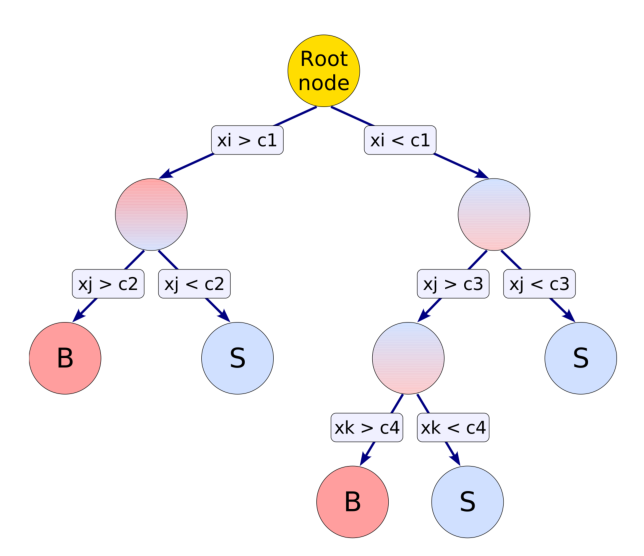
\includegraphics[width=0.75\textwidth]{figs/background-estimation/decisionTree.pdf}
\caption{A simple decision tree where repeated cuts a member of the set of variables $\textbf{x}$ are perfomed until a leaf node is reached and the object is classified as either signal (S) or background (B)~\cite{Hocker:2007ht}.
}
\label{fig:decisionTree}
\end{figure}

As the decision criterion for each node is dependent on the decisions of the preceding nodes, decision trees have the potential to obtain better separation between signal and background processes through individual cuts on isolated variables.
Without any prior knowledge of the system however, a single isolated tree is not expected to be an efficient classifier.
Despite this however, such a weak learner will still contain some knowledge about the underlying structure of the classification problem.

\emph{Boosting} aims to exploit this knowledge by using an ensemble of repeatedly trained weak learners to produce a more effective classifier.
Following each training iteration the dataset is reweighted based on the success of the previous classifiers in order to force the weak learners to attempt to classify objects that are harder to identify.
At the end of this process a weighted average of all the weak learners are combined to produce a single strong learner.

Therefore by extending boosting to decision trees, the resultant forest of Boosted Decision Trees produces a classifier that is both much more effective and resilient to fluctuations in the training sample than one created by a single tree.
Typically the classifier produced by a BDT takes the form of a single discriminator whose response ranges between $-1$ to $+1$, denoting completely background-like and signal-like objects, respectively.

BDTs are however, particularly sensitive to the effects of \emph{overtraining}.
This phenomena occurs when a BDT is overly optimised on correctly classifying events from the training dataset and results in the poor classification of unseen data.
In order to minimise the potential of overtraining occurring, the signal and background process samples are typically split into training and testing samples.
The testing samples are not trained on in order to check the effectiveness of the BDT trained using the training sample.

Two of the most common boosting algorithms used with decision trees are the Adaptive Boosting (\emph{AdaBoost})~\cite{Friedman:additivelogistic} and \emph{Gradient Boosting}~\cite{Friedman:greedyfunction,Friedman:GradientBoosting} algorithms.
Adaboost adjusts the weighting assigned to both  misclassified objects and the best performing weak learners after each iteration so that the best learners are trained to correctly identify the most difficult objects.
In contrast, gradient boosting uses gradient descent following each iteration to determine the residuals of the objects in order to focus on correctly classifying the objects with the largest residuals.

A number of studies were performed to determine the optimal settings for this analysis.
These included the evaluation of:

\begin{itemize}
\item a number of different boosting algorithms;
\item which simulated background processes should be included in the training processes;
\item whether or not multiple BDTs trained on separate backgrounds would be more effective than a single BDT;
\item how to determine which input variables possessed the greater discriminating power;
\item and which \emph{hyperparameters}, the set of options used to control BDT behaviour, and associated values gave the optimal classification performance.
\end{itemize}

It was determined that the \emph{eXtreme Gradient Boosting} (XGBoost) implementation of the Gradiant Boost algorithm for a single BDT trained on all the MC simulation samples gave the optimal performance for this search~\cite{xgboost}.

\subsection{BDT Optimisation and Evaluation}\label{subsec:bdtOpt}
The methods used for determining the optimal input variables and model hyperparameters for this BDT are described in the following subsection.
Both the input variables and model hyperparameters were chosen separately for $ee$ and $\mu\mu$ channels and all the simulated MC samples were considered.

Once the optimisation is complete, the BDT is trained.
The BDT produces the output discriminant for each of the data and simulation samples considered.
These output discriminant distributions are used to extract the signal strength and its statistical significance, as described in Chapter~\ref{chapter:results}.

\subsubsection*{BDT Input Variable Optimisation}
From the selected reconstructed physics objects, a large number of possible input variables were constructed and considered as inputs for the BDT.
Training a BDT with all of the possible input variables increases its vulnerability to overtraining, as correlated input variables are considered multiple times and statistical fluctuations in poorly discriminating input variables may give the illusion of discriminative power.

In order to determine the optimal set of input variables, recursive feature elimination was used to those that had the greatest discriminating power between signal and background~\cite{Guyon2002}.
This process iteratively removes the least important input variable and re-trains the BDT until every input variable has been ranked in order of their removal.
From this process, the highest ranked input variables are identified for use in the BDT.

The input variables chosen by this method for the $ee$ and $\mu\mu$ channels are given in table~\ref{tab:selectedBdtVariables}.
As can be seen in Figures~\ref{fig:corr_ee}-\ref{fig:corr_mumu}, the majority of these variables are weakly correlated, as indicated by pale squares, signifying that they provide unique and useful information to the BDT.
Table~\ref{tab:allBdtVariables} in Appendix~\ref{app:bdt} provides a list of all the input variables that were considered.

\begin{table}[htb]
\topcaption {The name and descriptions of the variables chosen by recursive feature elimination to be used as input to the BDT to discriminate between potential tZq signal events and the dominant backgrounds.
}
\label{tab:selectedBdtVariables}
  \centering
% This increases column spacing.
\resizebox{\textwidth}{!}{
% This right-aligns numbers in column, but centers them under column title.
\begin{tabular}{cccc}
   \hline\
   \multirow{2}{*}{\textbf{Input variable}} & \multirow{2}{*}{\textbf{Description}} & \multicolumn{2}{c}{\textbf{Discriminating Power}}  \\
   & & \textbf{$ee$} & \textbf{$\mu\mu$} \\
   \hline
    topMass & Reconstructed top quark mass & $1.449 \times 10^{-1}$  & $1.794 \times 10^{-1}$  \\
    zMass & Reconstructed Z boson mass & $1.202 \times 10^{-1}$  & $1.372 \times 10^{-1}$  \\
    jetMass & Total mass of every jet in an event & $1.079 \times 10^{-1}$  & $9.304 \times 10^{-2}$  \\
    met & Missing transverse energy & $9.100 \times 10^{-2}$  & $9.382 \times 10^{-2}$  \\
    bTagDisc & Leading b-tagged jet CSVv2 discriminant & $6.773 \times 10^{-2}$  & $6.372 \times 10^{-2}$ \\ 
    leadJetPt & Leading jet \pt & $6.093 \times 10^{-2}$ & $4.926 \times 10^{-2}$  \\ 
    jjDelR & $\Delta R$ between the leading jets & $5.300 \times 10^{-2}$  & $3.987 \times 10^{-2}$  \\ 
    wPairMass & Reconstructed W boson mass & $5.093 \times 10^{-2}$ & $4.808 \times 10^{-2}$  \\
    lepHt & ${\ensuremath{H_{\mathrm{T}}}}$ of the Z boson's leptons & $4.620\times 10^{-2}$ & $5.395 \times 10^{-2}$ \\
    totHtOverPt & Total ${\ensuremath{H_{\mathrm{T}}}}$ divided by total \pt & $4.487 \times 10^{-2}$  & $3.284 \times 10^{-2}$  \\
    leadJetEta & Leading jet $\eta$ & $4.467 \times 10^{-2}$ & $6.138 \times 10^{-2}$  \\
    jetHt & ${\ensuremath{H_{\mathrm{T}}}}$ of all the jets in an event & - & $5.629 \times 10^{-2}$ \\ 
    secJetPt & Second jet \pt & $4.453 \times 10^{-2}$ & -  \\
    zlQuark2DelR & $\Delta R$ between the leading lepton and W boson's subleading jet & $4.093\times 10^{-2}$ & - \\
    thirdJetPt & Third jet \pt & $3.720 \times 10^{-2}$  & $3.753 \times 10^{-2}$  \\ 
    zlb1DelR & $\Delta R$ between the leading lepton and leading b-tagged jet & - & $3.245 \times 10^{-2}$ \\    
    zEta & Reconstructed Z boson $\eta$ & - & $2.111 \times 10^{-2}$ \\
    zlb2DelR & $\Delta R$ between subleading lepton and leading b-tagged jet & $2.627\times 10^{-2}$ & - \\
    fourthJetPt & Fourth jet \pt & $1.873 \times 10^{-2}$ & - \\ 
    \hline
 \end{tabular}}
\end{table}

\begin{figure}[h]
\centering
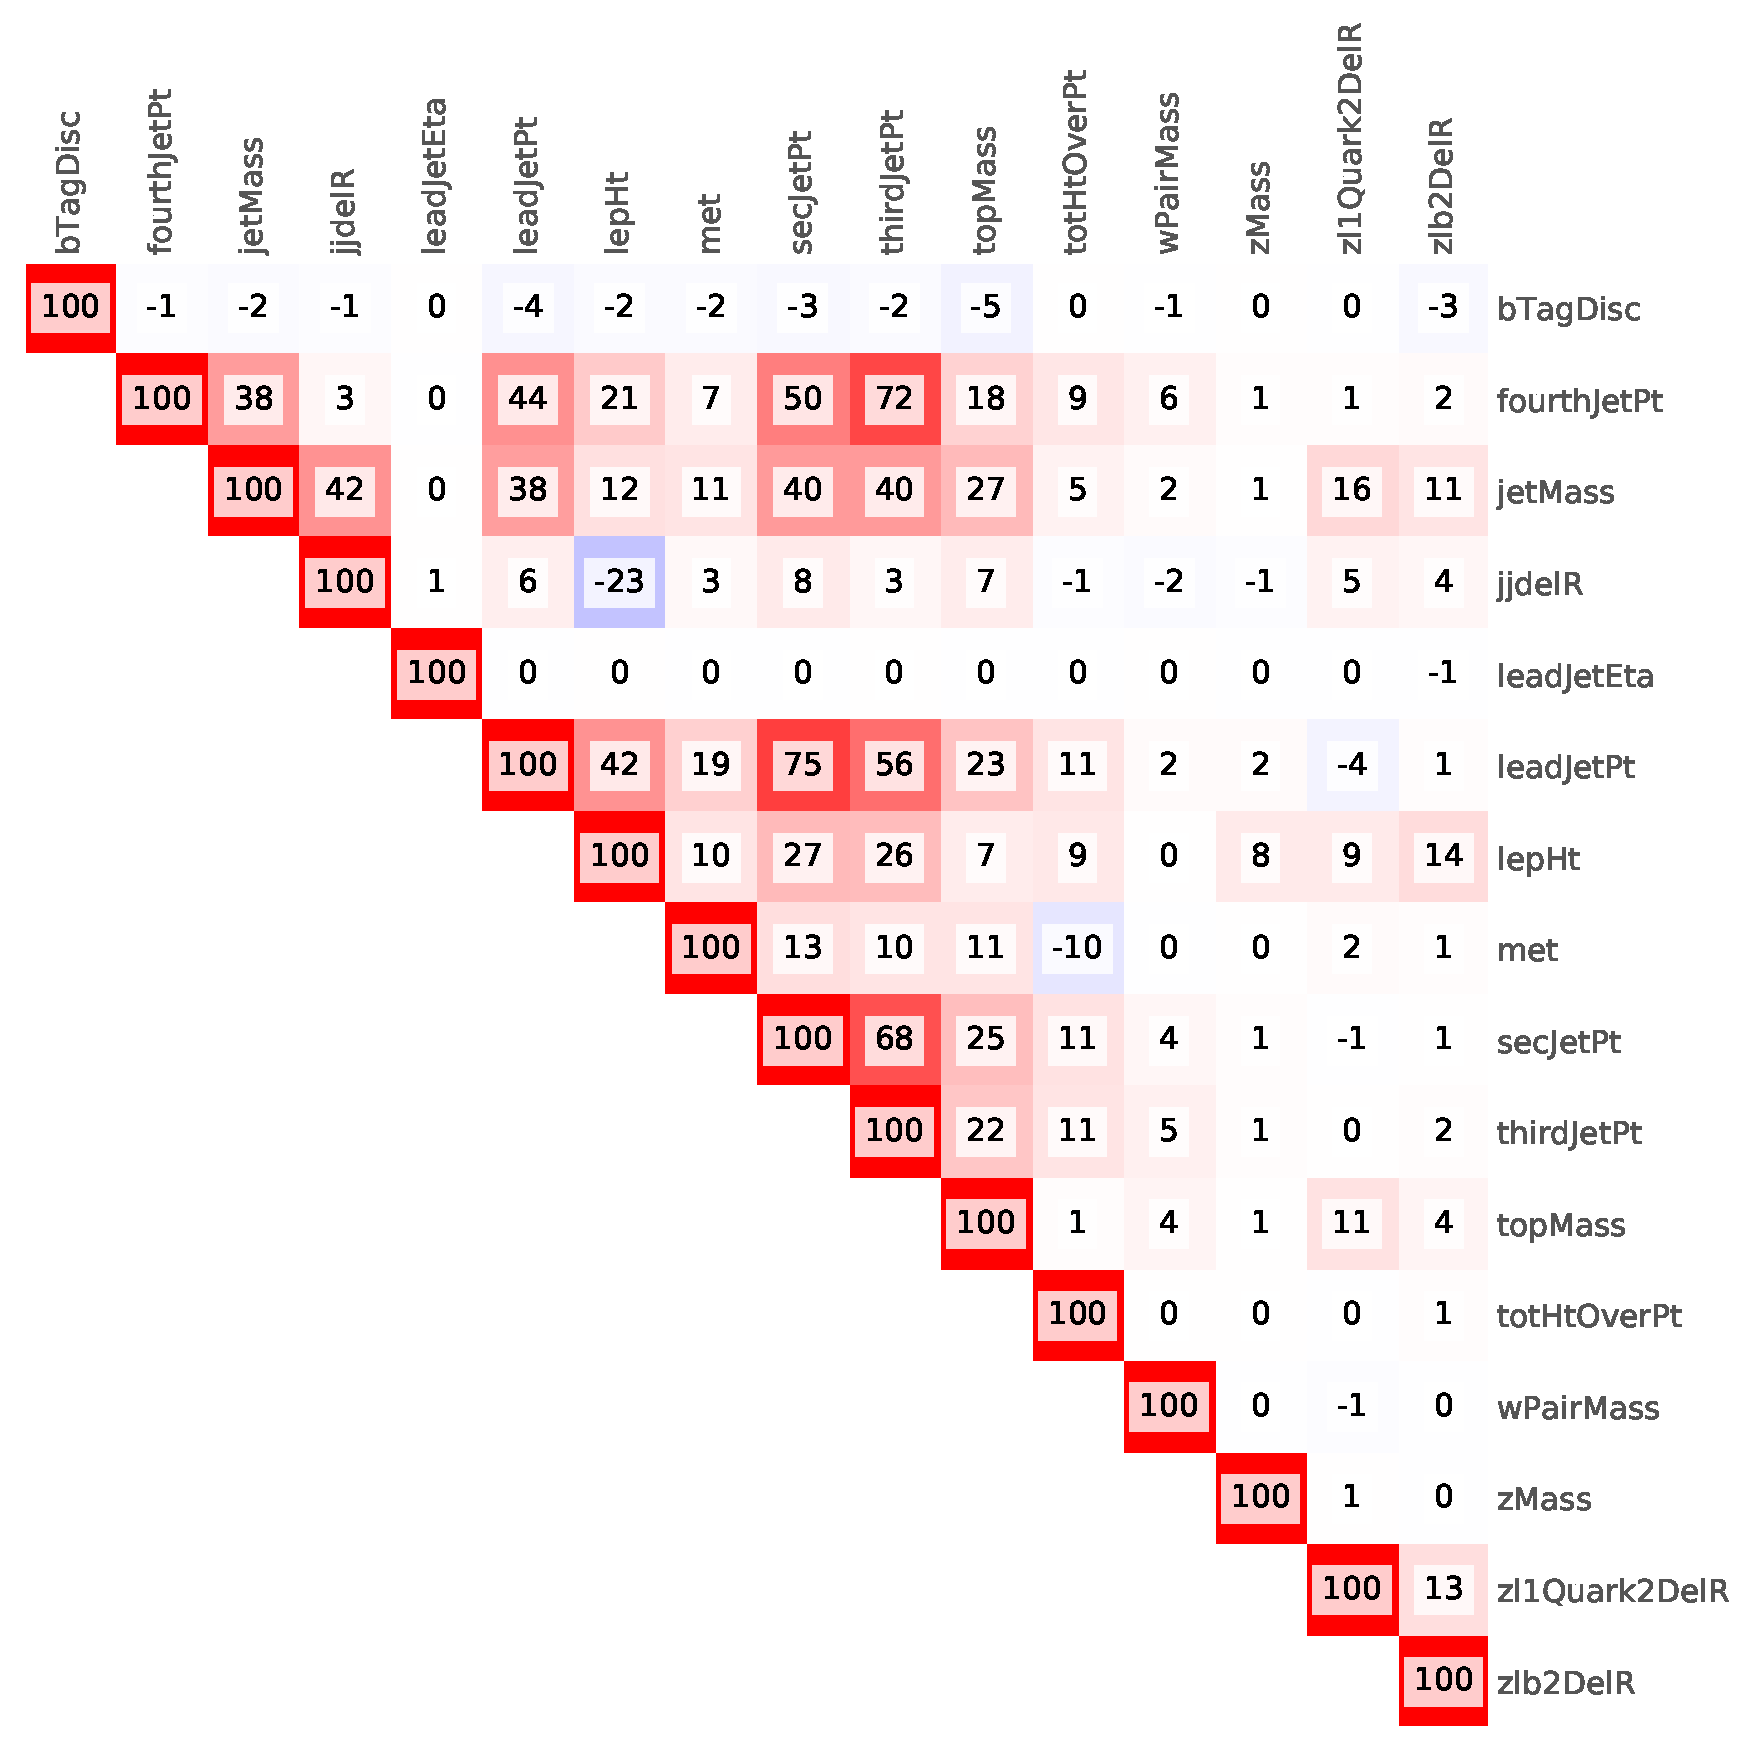
\includegraphics[width=0.7\textwidth]{figs/background-estimation/plots/corr_sig_ee.pdf}
\\
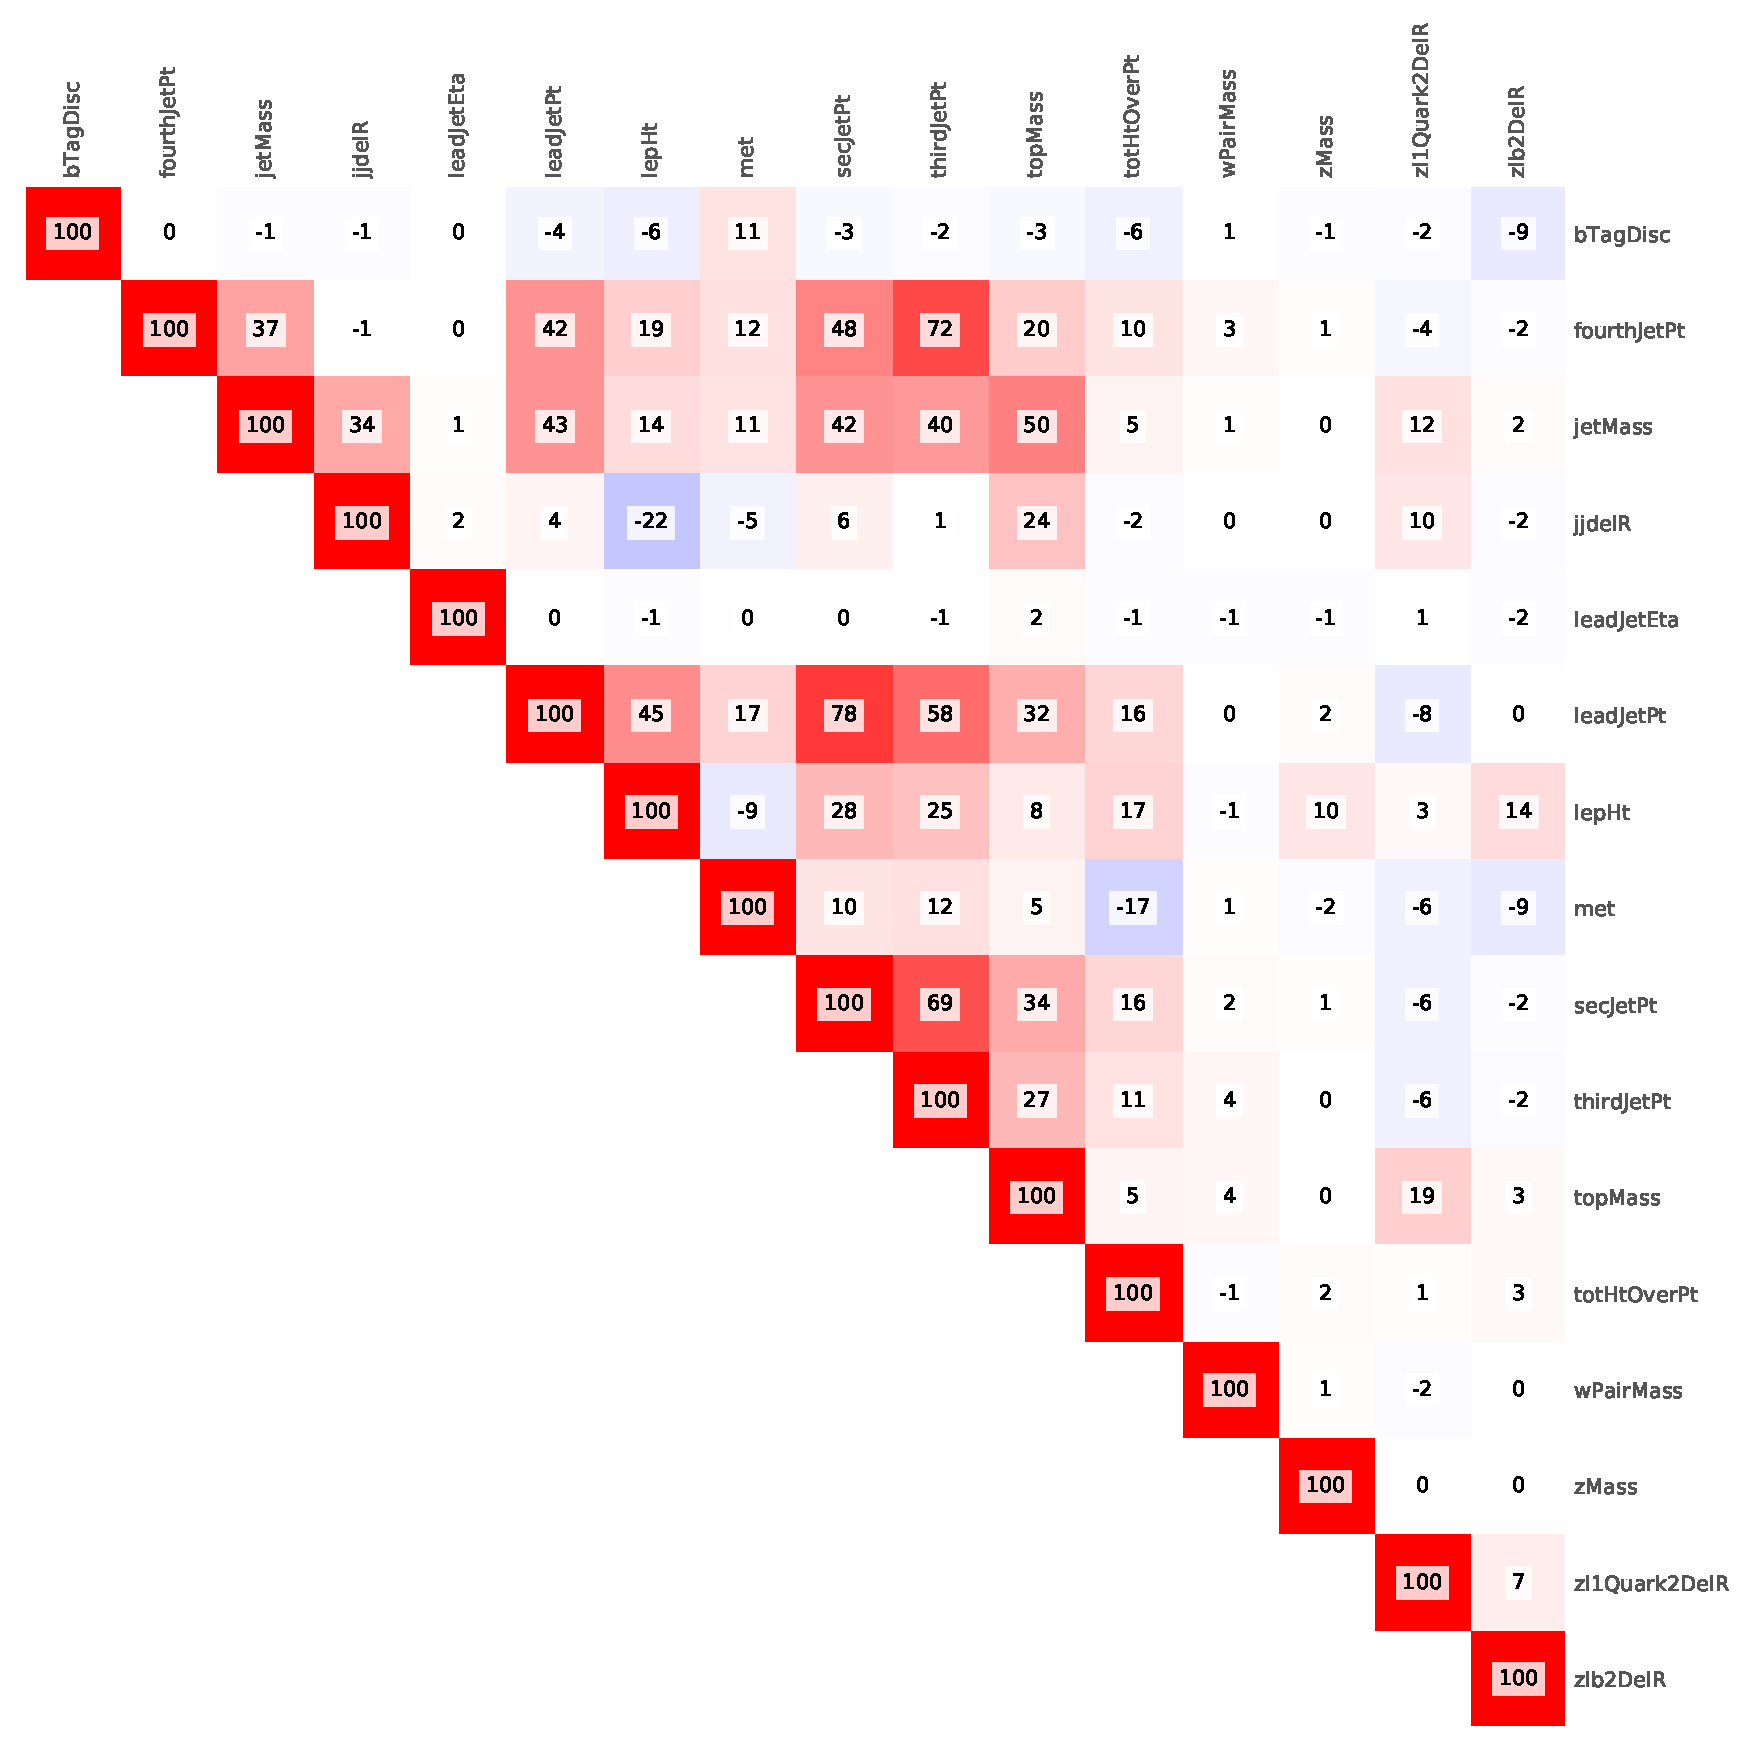
\includegraphics[width=0.7\textwidth]{figs/background-estimation/plots/corr_bkg_ee.pdf}
\caption{
The correlations between the input variables chosen for use with the BDT for the signal (top) and background (bottom) samples for the $ee$ channel.}
\label{fig:corr_ee}
\end{figure}

\begin{figure}[h]
\centering
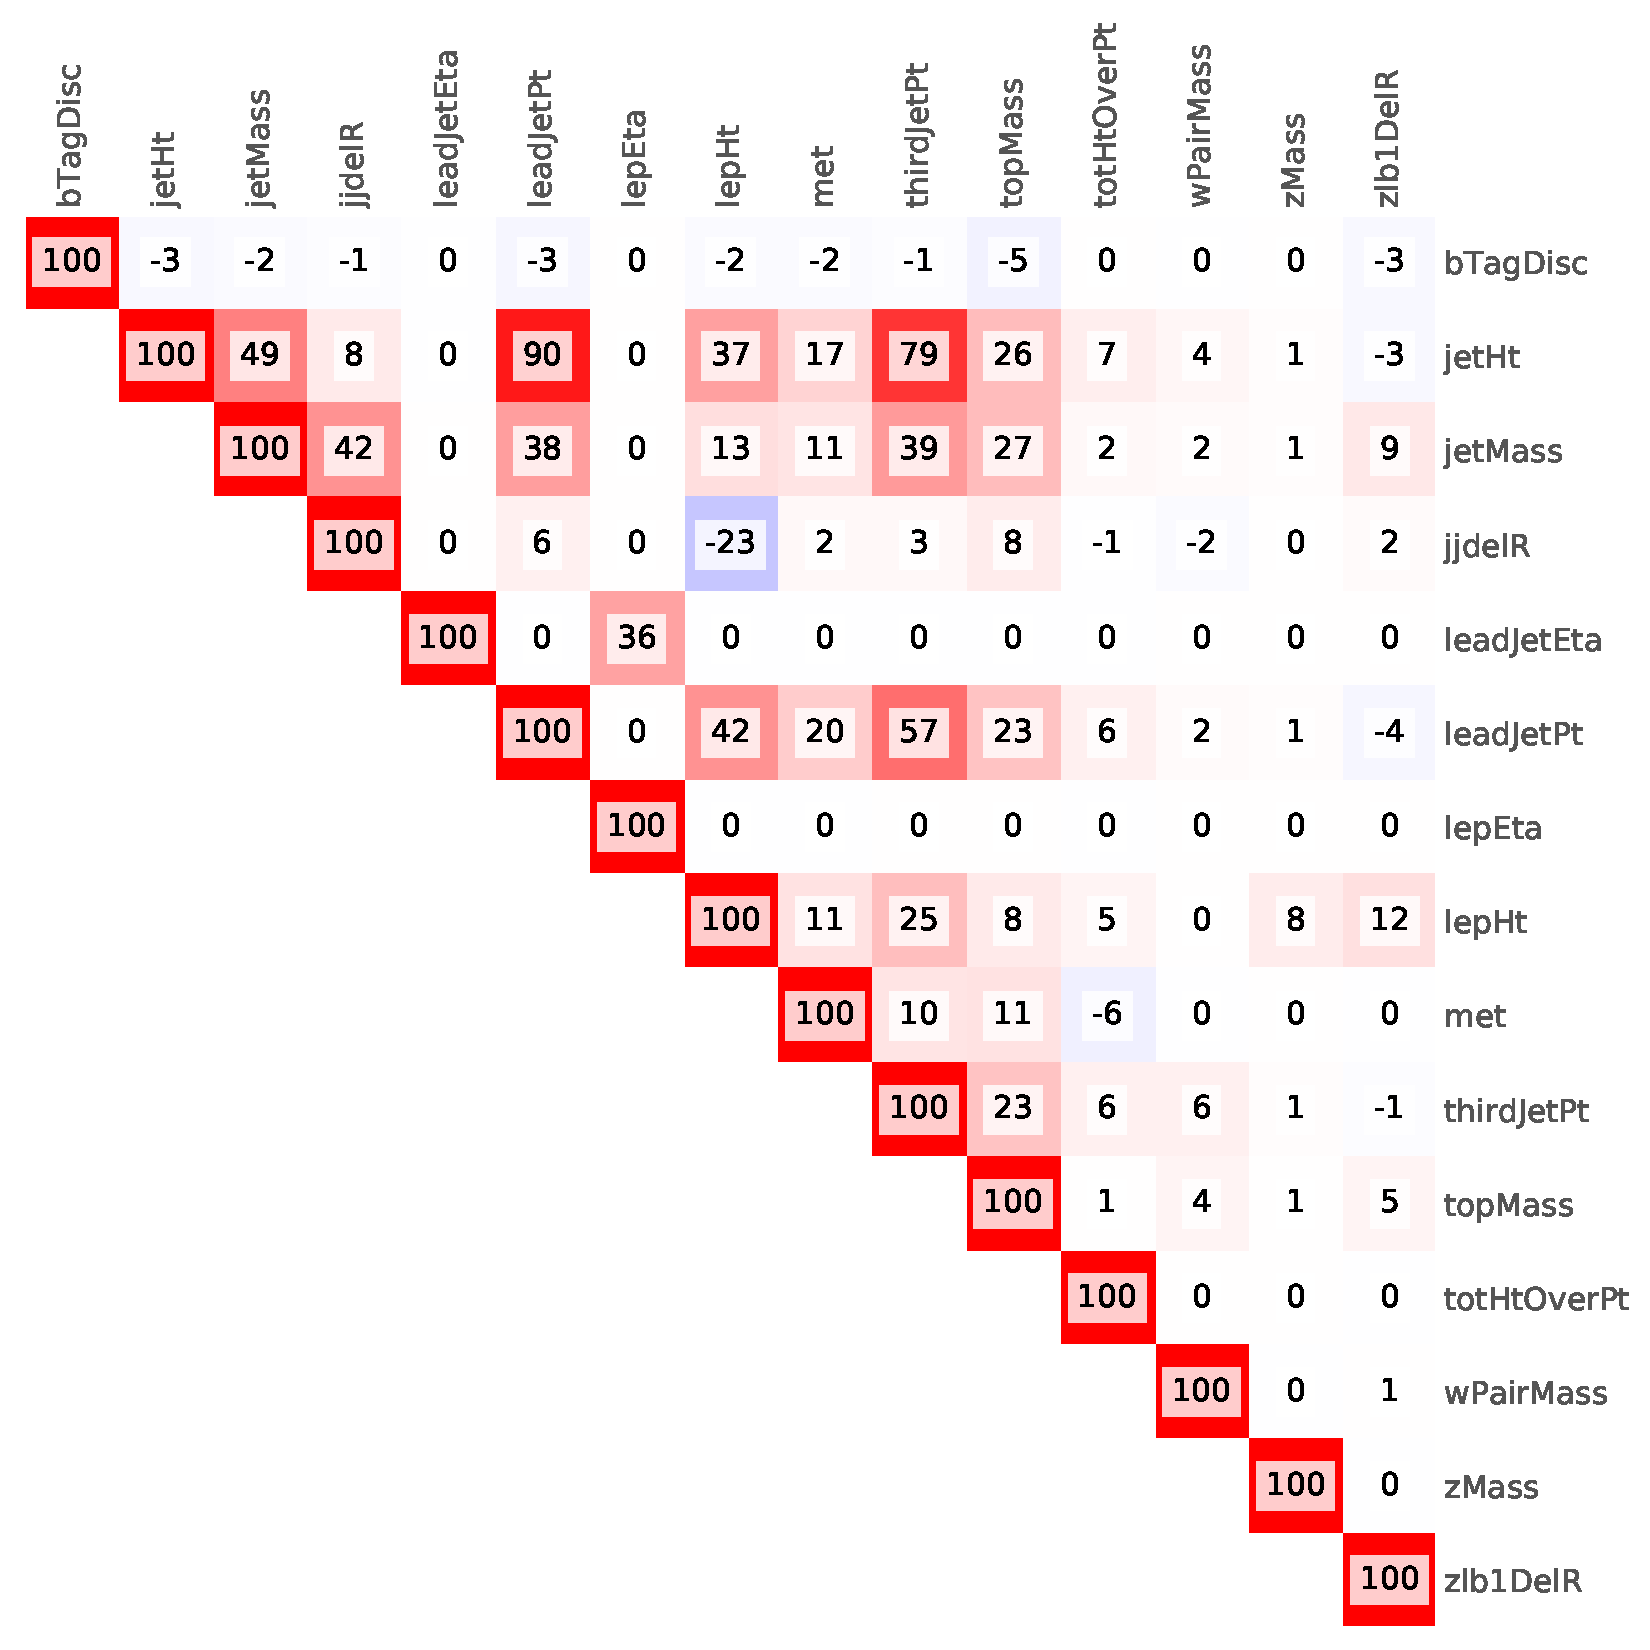
\includegraphics[width=0.7\textwidth]{figs/background-estimation/plots/corr_sig_mumu.pdf}
\\
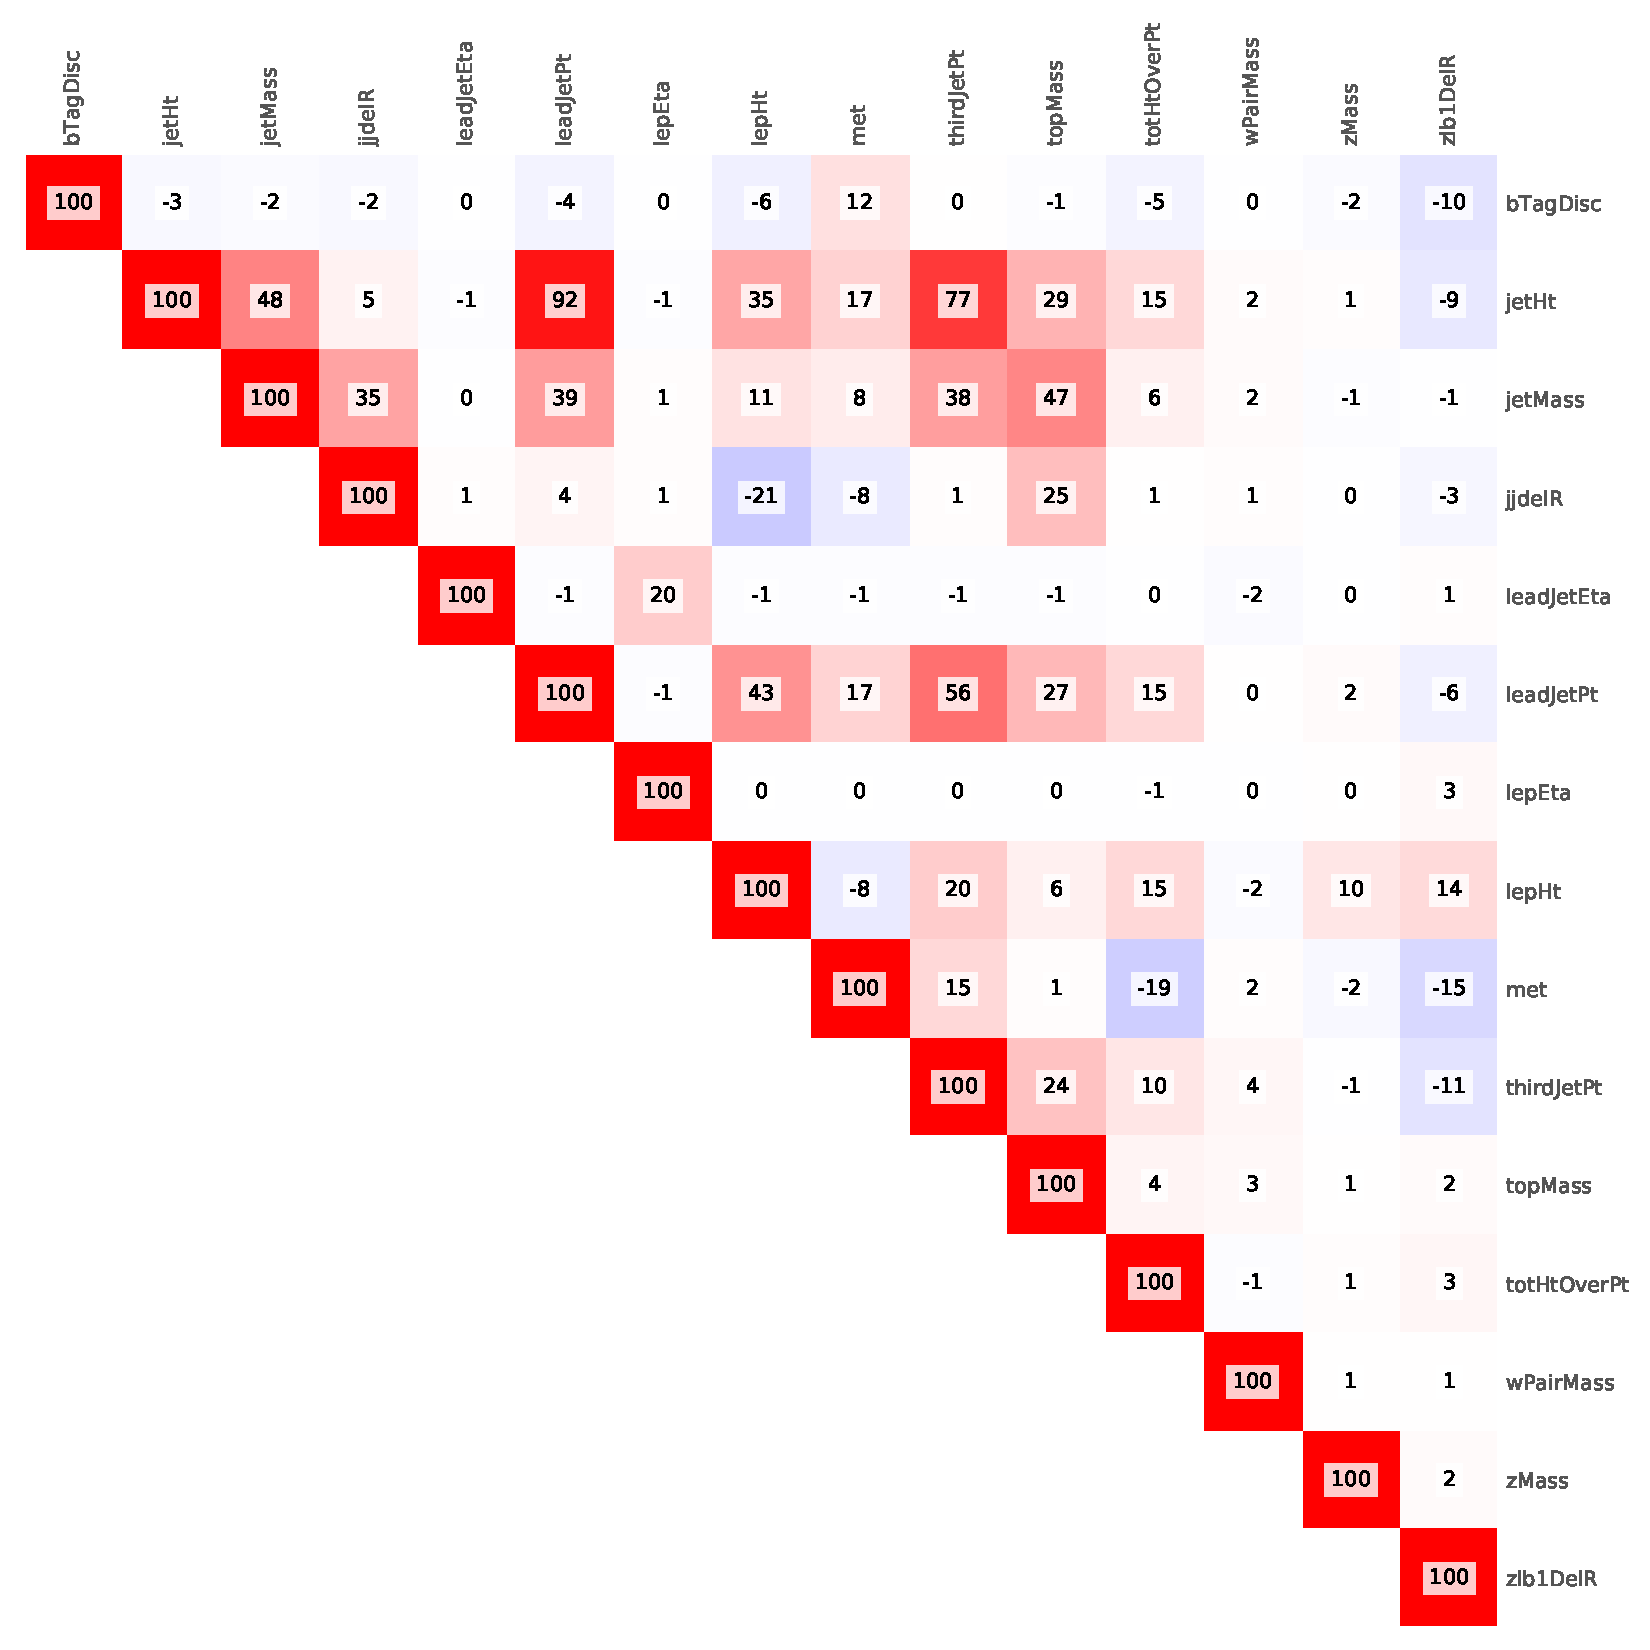
\includegraphics[width=0.7\textwidth]{figs/background-estimation/plots/corr_bkg_mumu.pdf}
\caption{
The correlations between the input variables chosen for use with the BDT for the signal (top) and background (bottom) samples for the $\mu\mu$ channel.}
\label{fig:corr_mumu}
\end{figure}

Figures~\ref{fig:inputFeaturesDataSimAgreement1},~\ref{fig:inputFeaturesDataSimAgreement2},~\ref{fig:inputFeaturesDataSimAgreement3},~\ref{fig:inputFeaturesDataSimAgreement4} and~\ref{fig:inputFeaturesDataSimAgreement5} show that good agreement was observed between simulation and data for the selected input variables.
Given the number of input variables used, when an input variable is used by both the $ee$ and $\mu\mu$ channels, only the distributions for the one of the two channels are given in this chapter.
The complete set of distributions for both channels is given in Appendix~\ref{app:bdt}.

\begin{figure}[h]
\centering
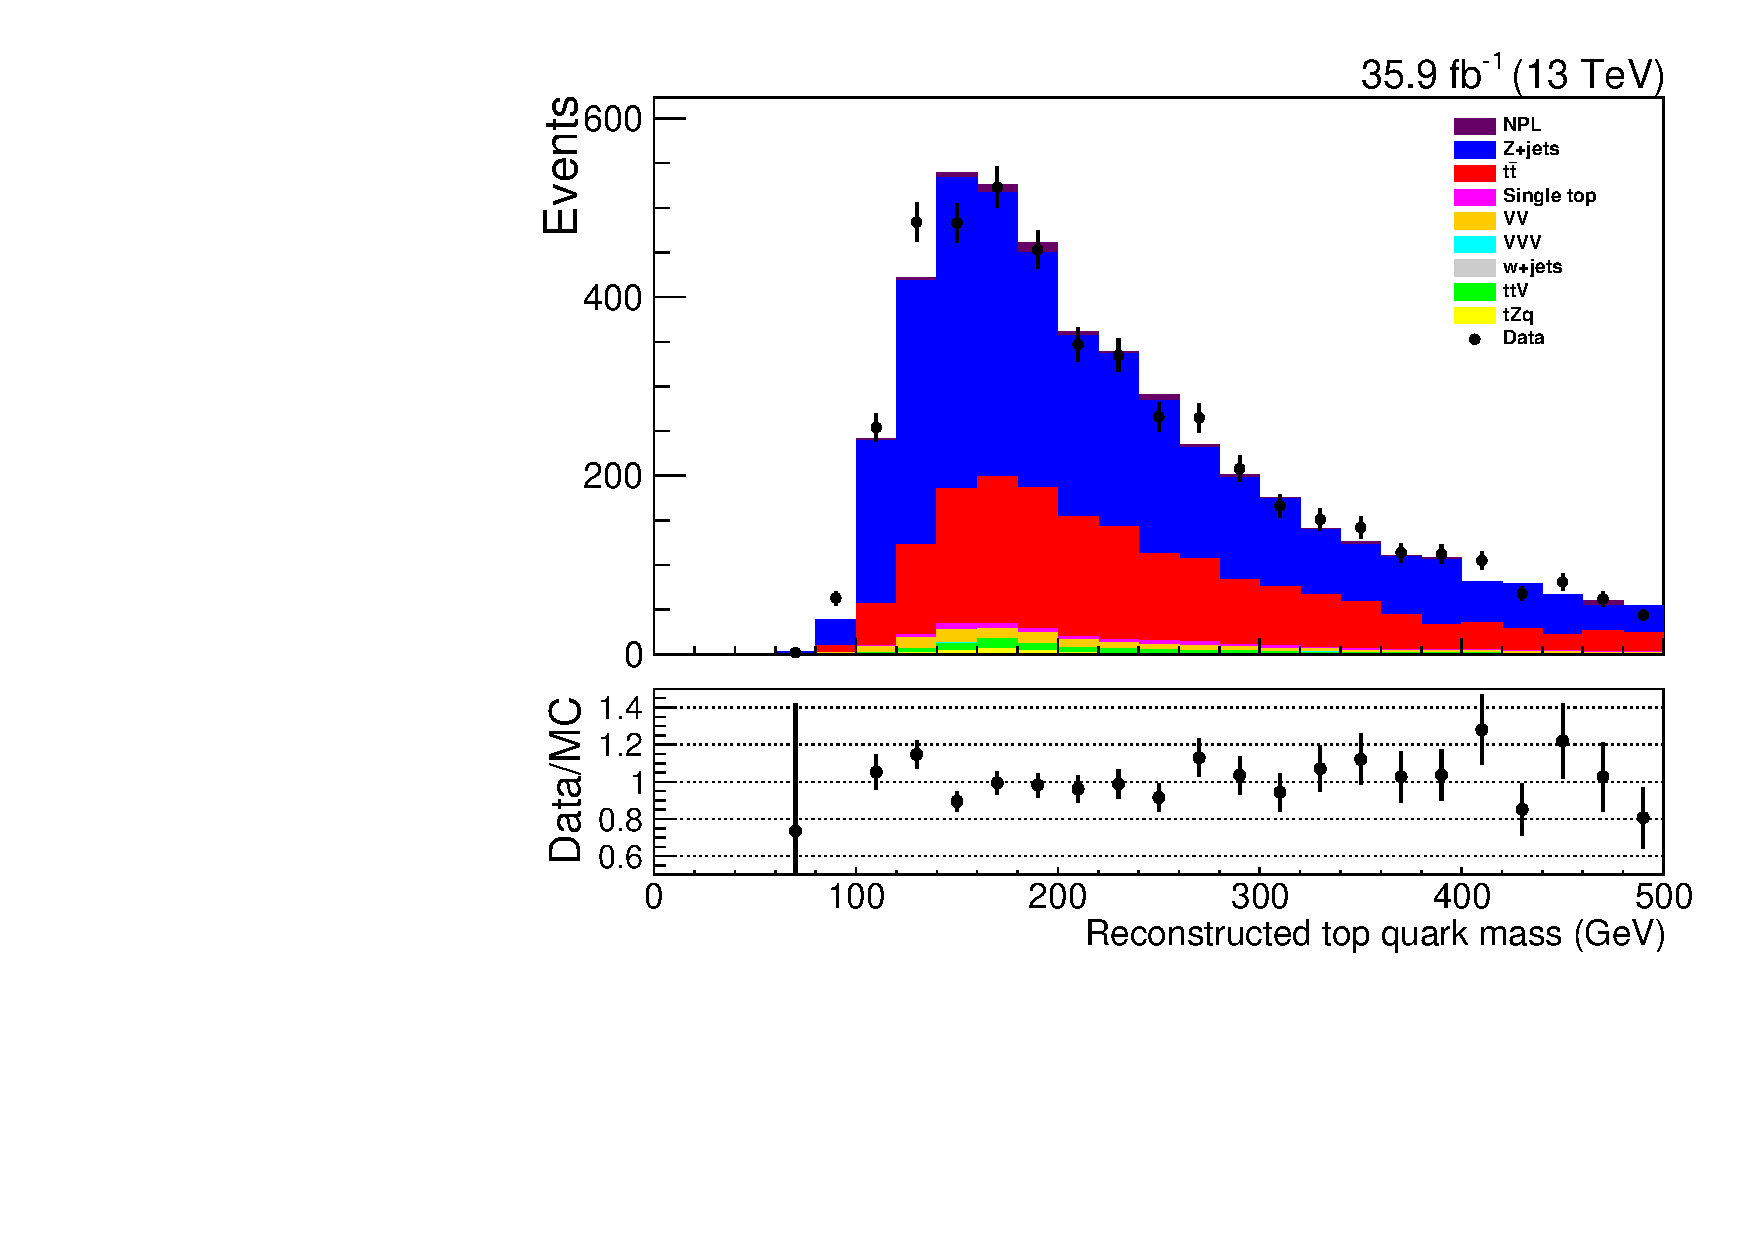
\includegraphics[width=0.47\textwidth]{figs/background-estimation/plots/unblinded/prompt_ee_ttbarInc/topMass_NPL_ee_wMass_ee.pdf}
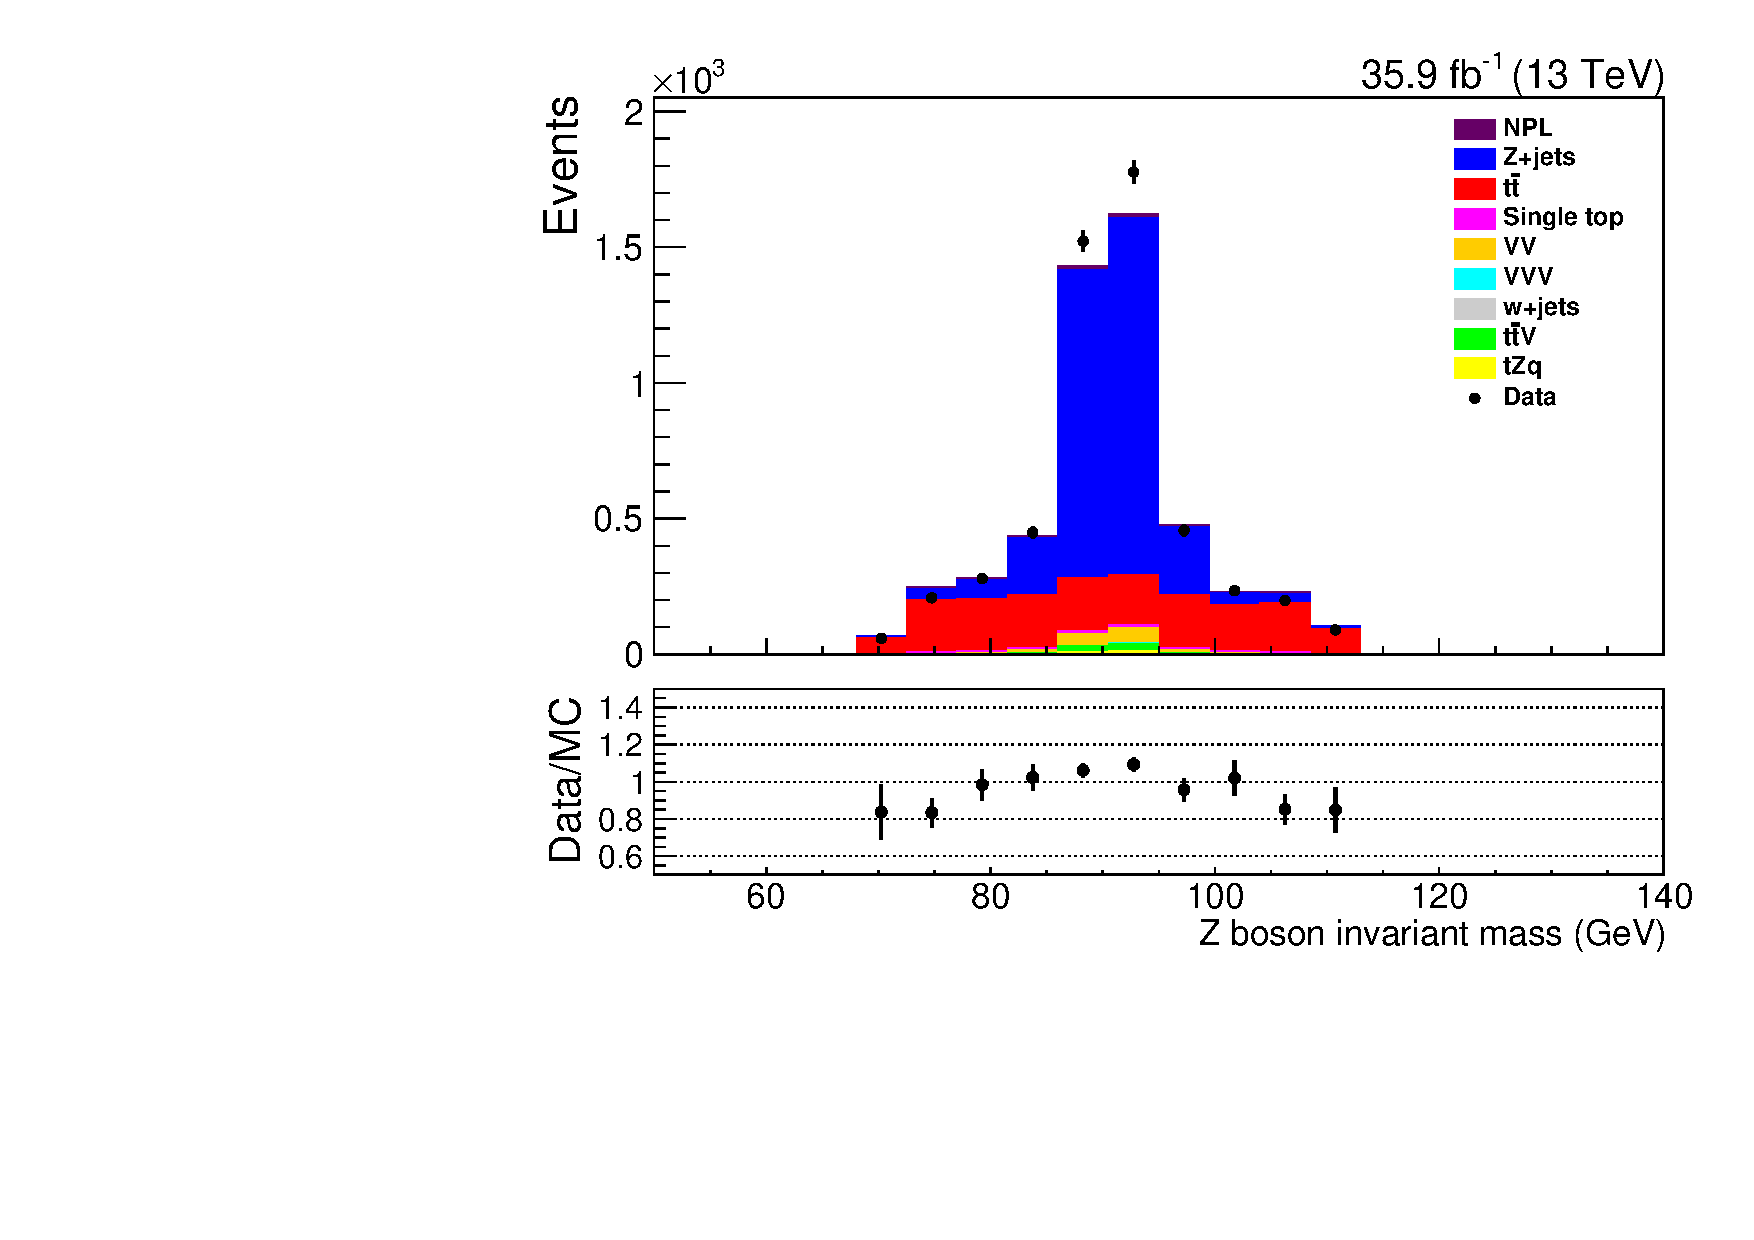
\includegraphics[width=0.47\textwidth]{figs/background-estimation/plots/unblinded/prompt_ee_ttbarInc/zPairMass_NPL_ee_wMass_ee.pdf}
\\
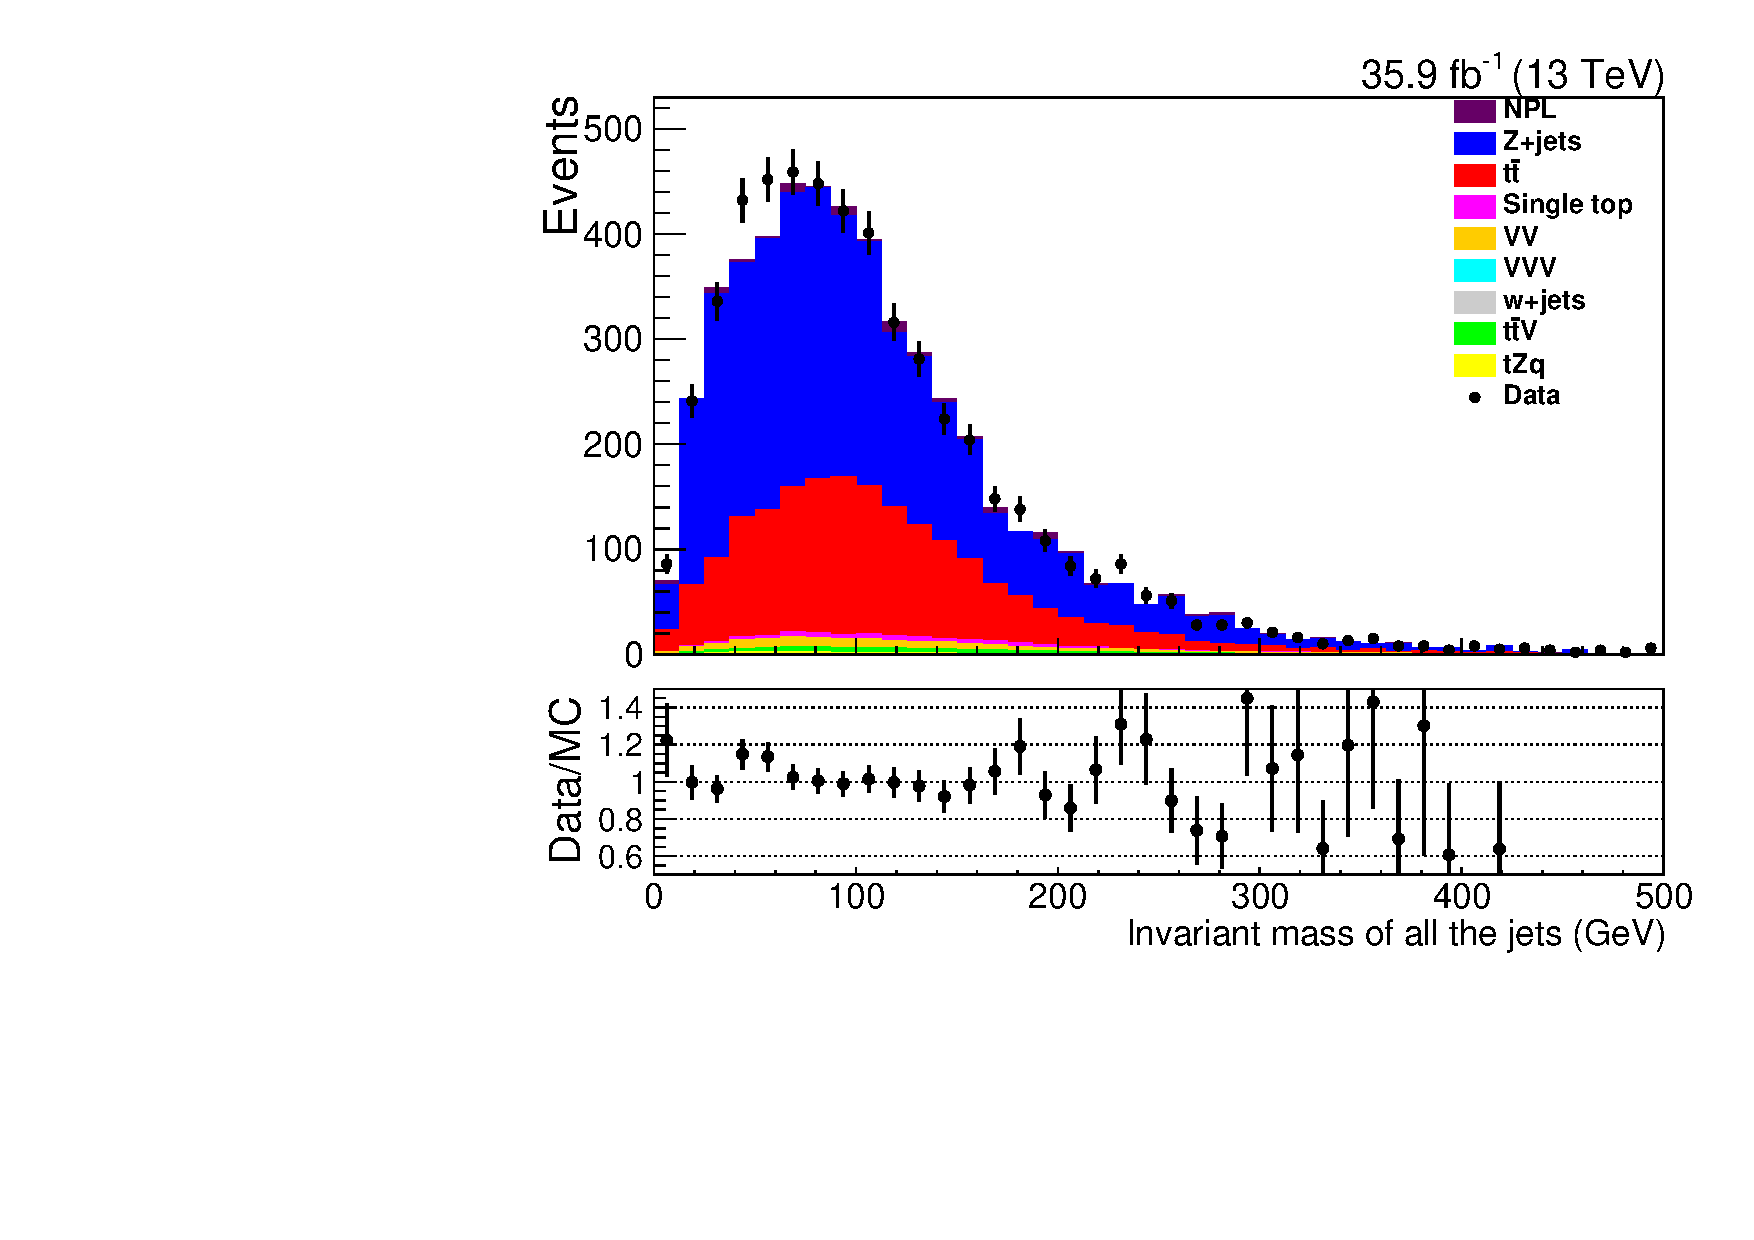
\includegraphics[width=0.47\textwidth]{figs/background-estimation/plots/unblinded/prompt_ee_ttbarInc/totalJetMass_NPL_ee_wMass_ee.pdf}
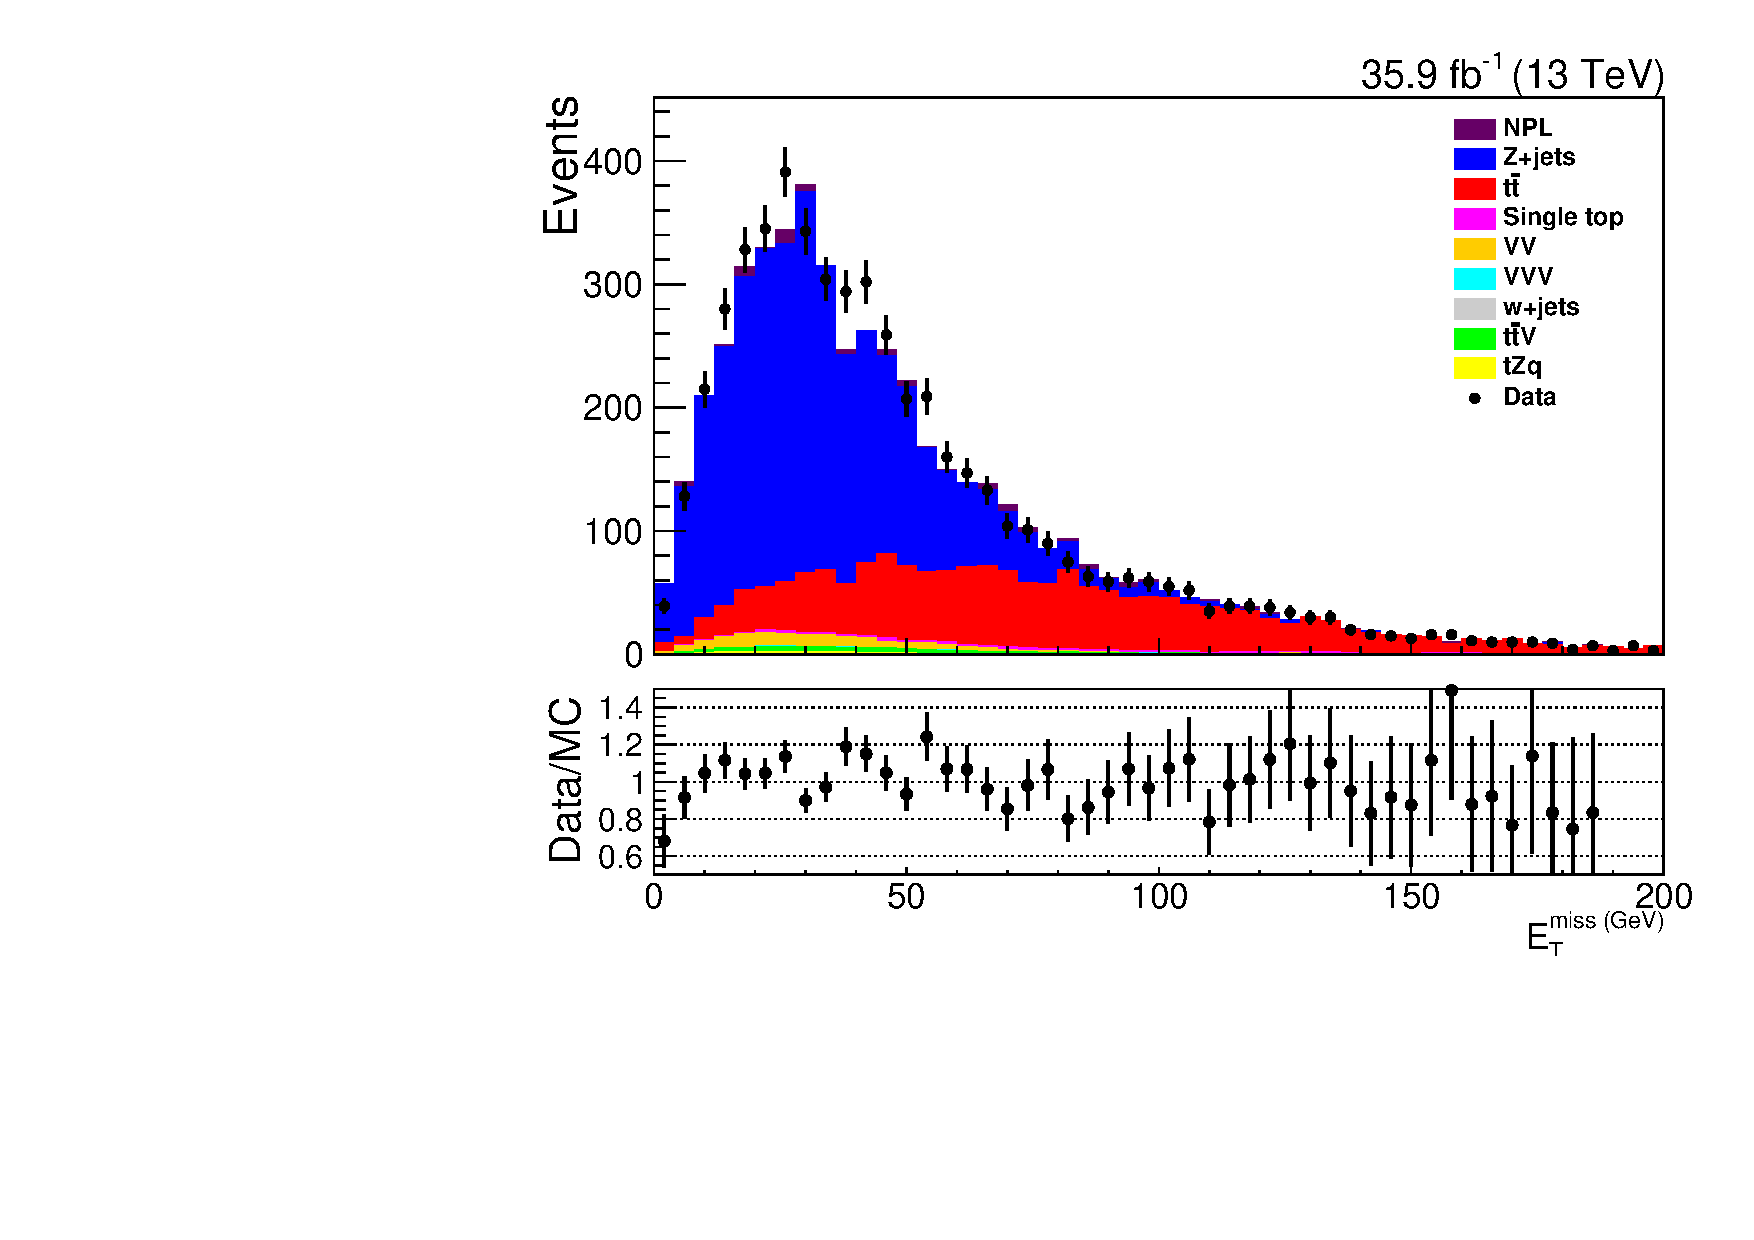
\includegraphics[width=0.47\textwidth]{figs/background-estimation/plots/unblinded/prompt_ee_ttbarInc/met_NPL_ee_wMass_ee.pdf}
\caption{
Reconstructed top mass, Z boson mass, total jet mass, and \MET distributions for the $ee$ channel comparing the agreement between data and simulation for the variables used as input variables in the BDT training.}
\label{fig:inputFeaturesDataSimAgreement1}
\end{figure}

\begin{figure}[h]
\centering
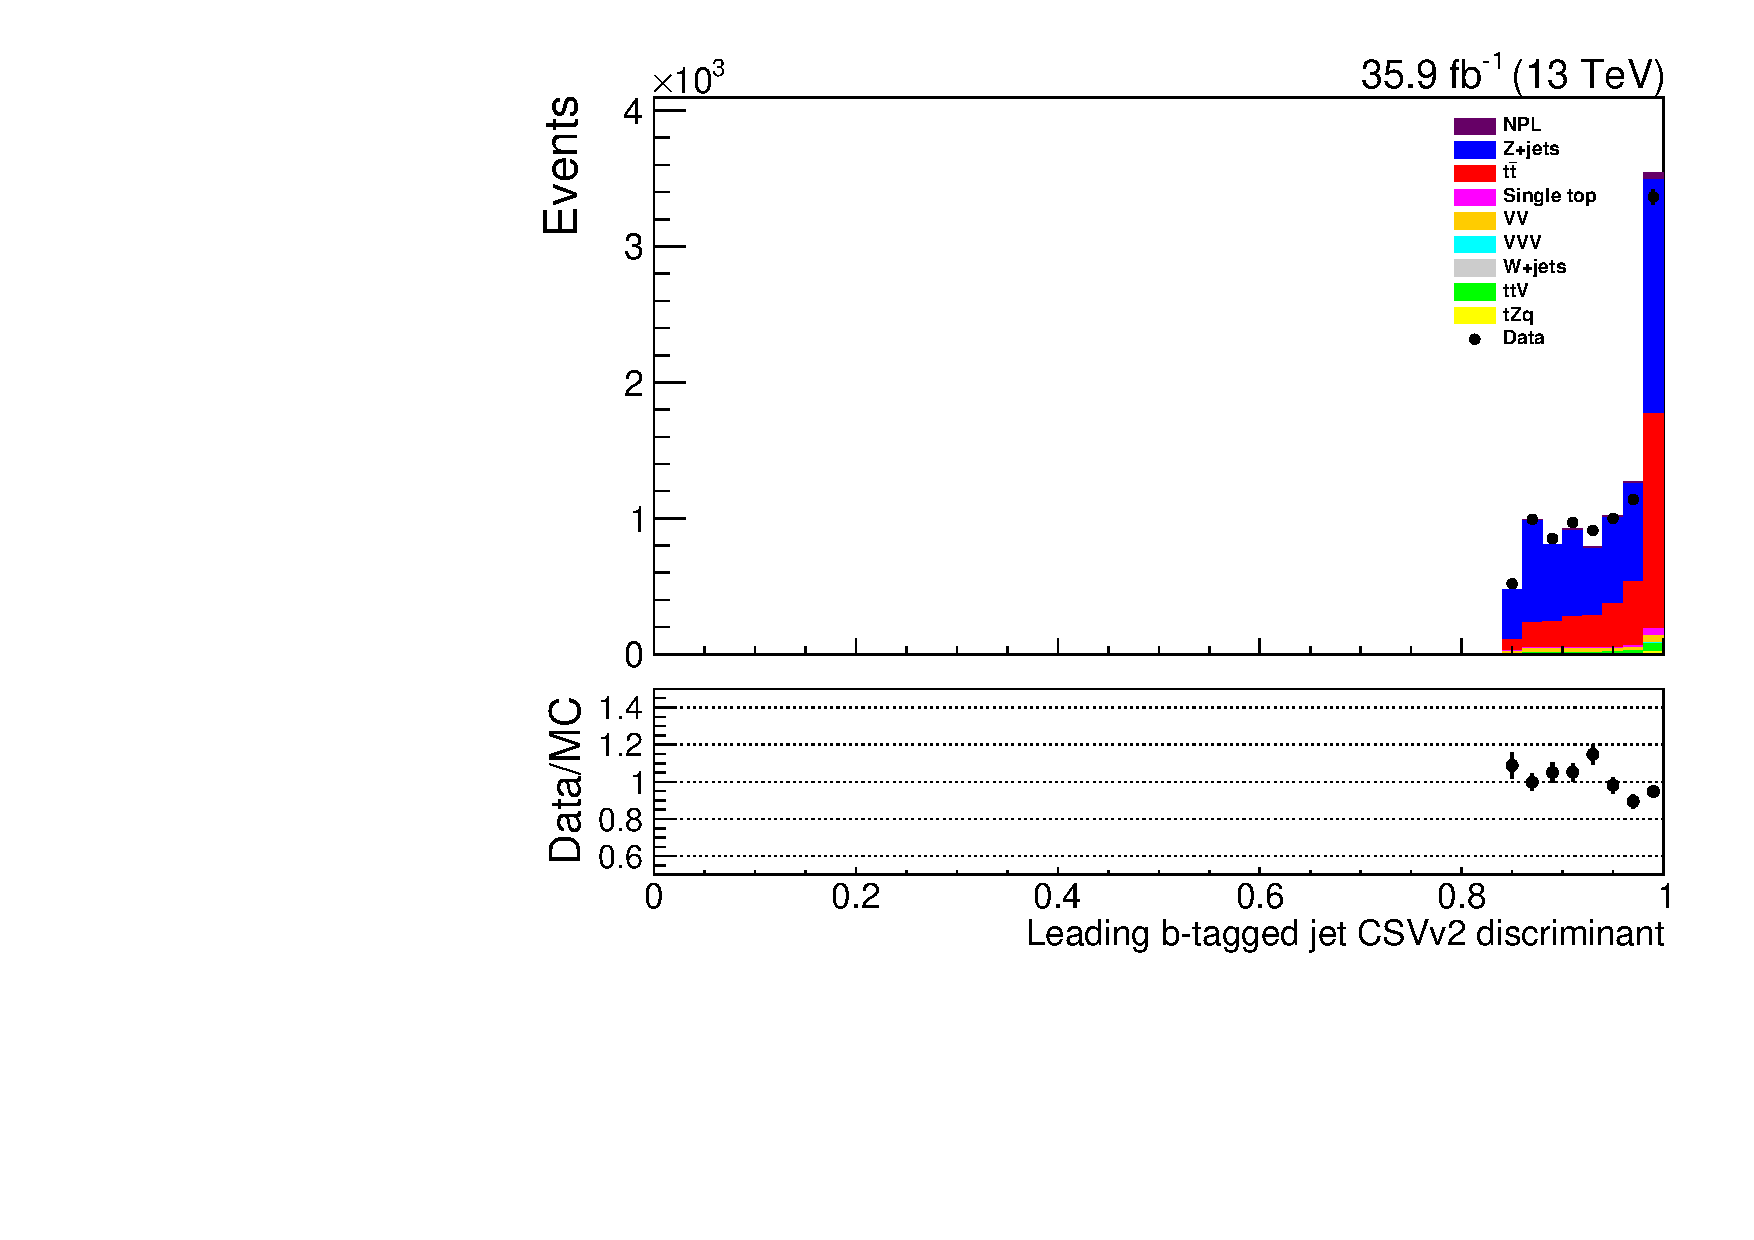
\includegraphics[width=0.47\textwidth]{figs/background-estimation/plots/unblinded/prompt_mumu_ttbarInc/bTagDisc_NPL_mumu_wMass_mumu.pdf}
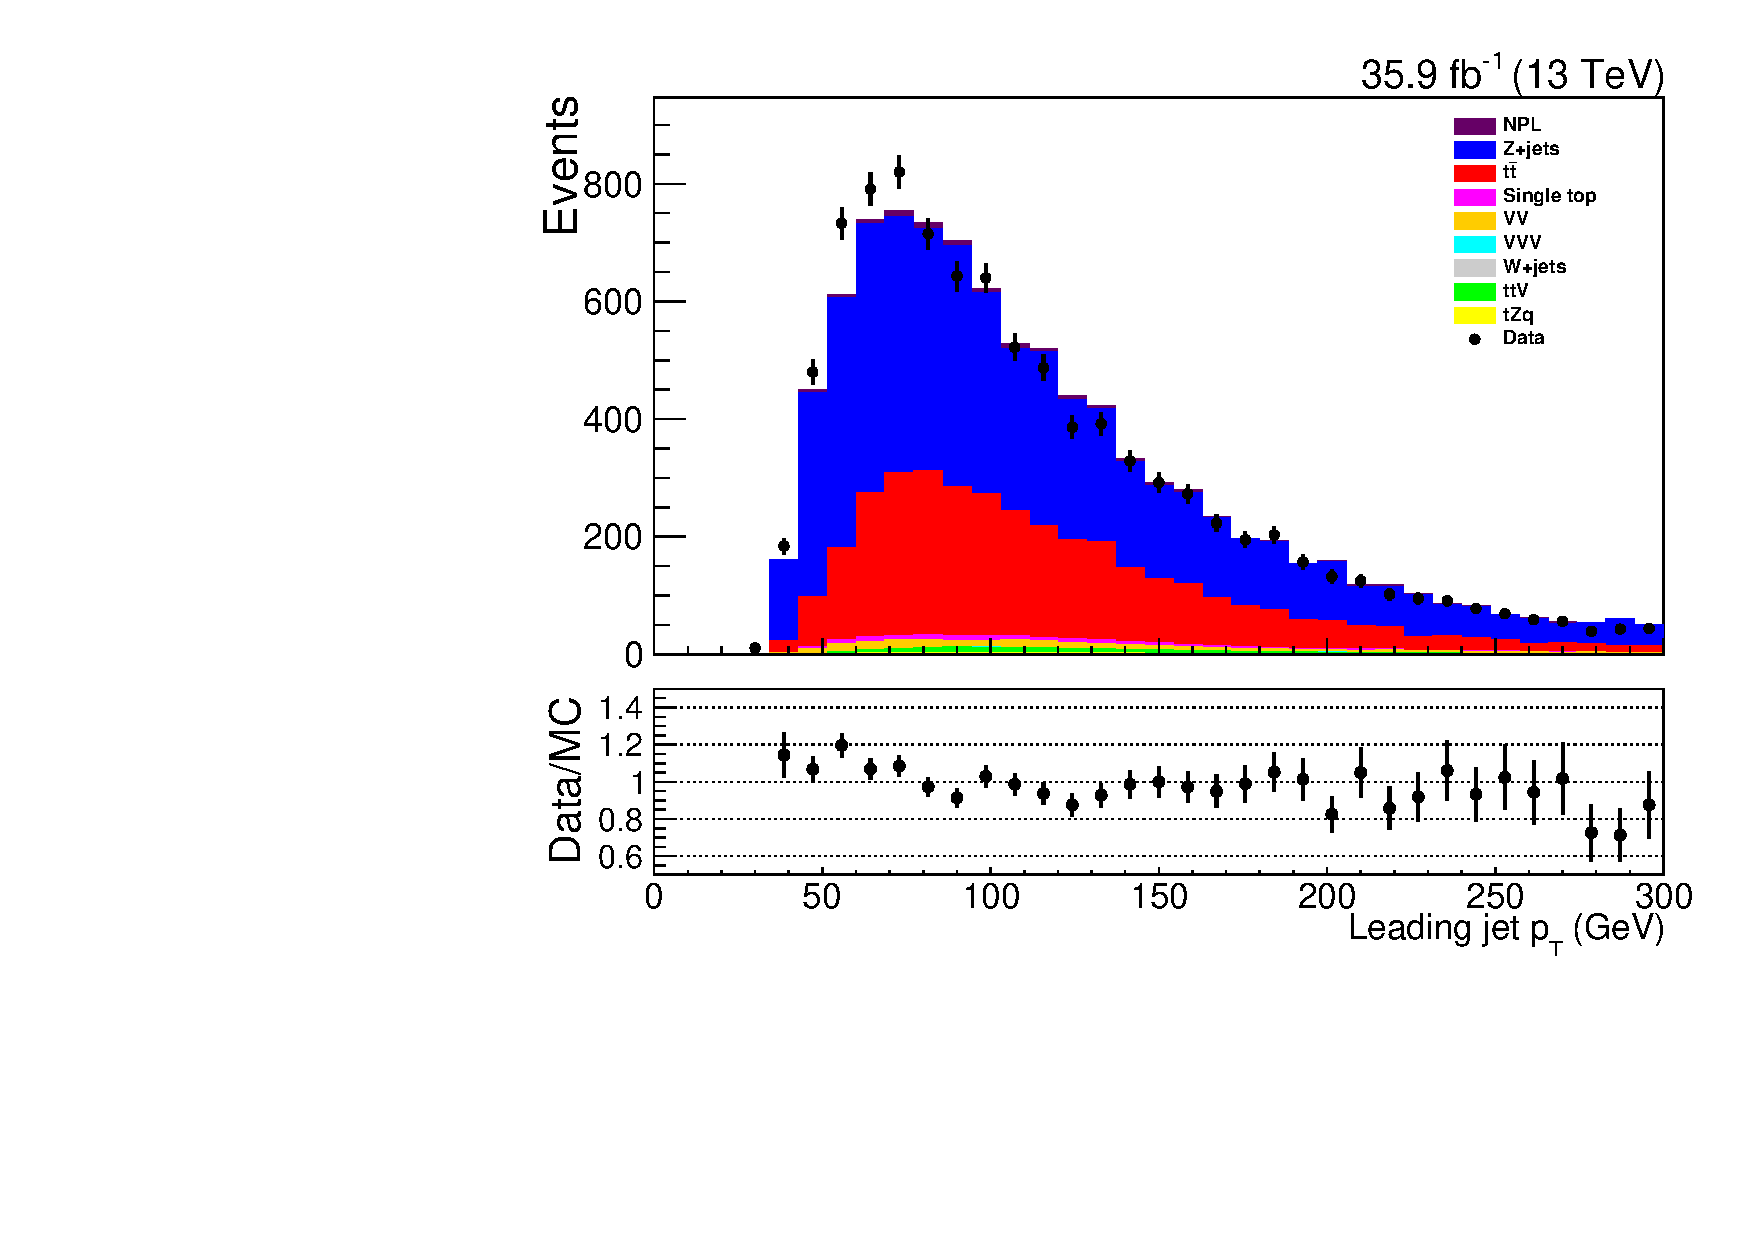
\includegraphics[width=0.47\textwidth]{figs/background-estimation/plots/unblinded/prompt_mumu_ttbarInc/leadingJetPt_NPL_mumu_wMass_mumu.pdf}
\\
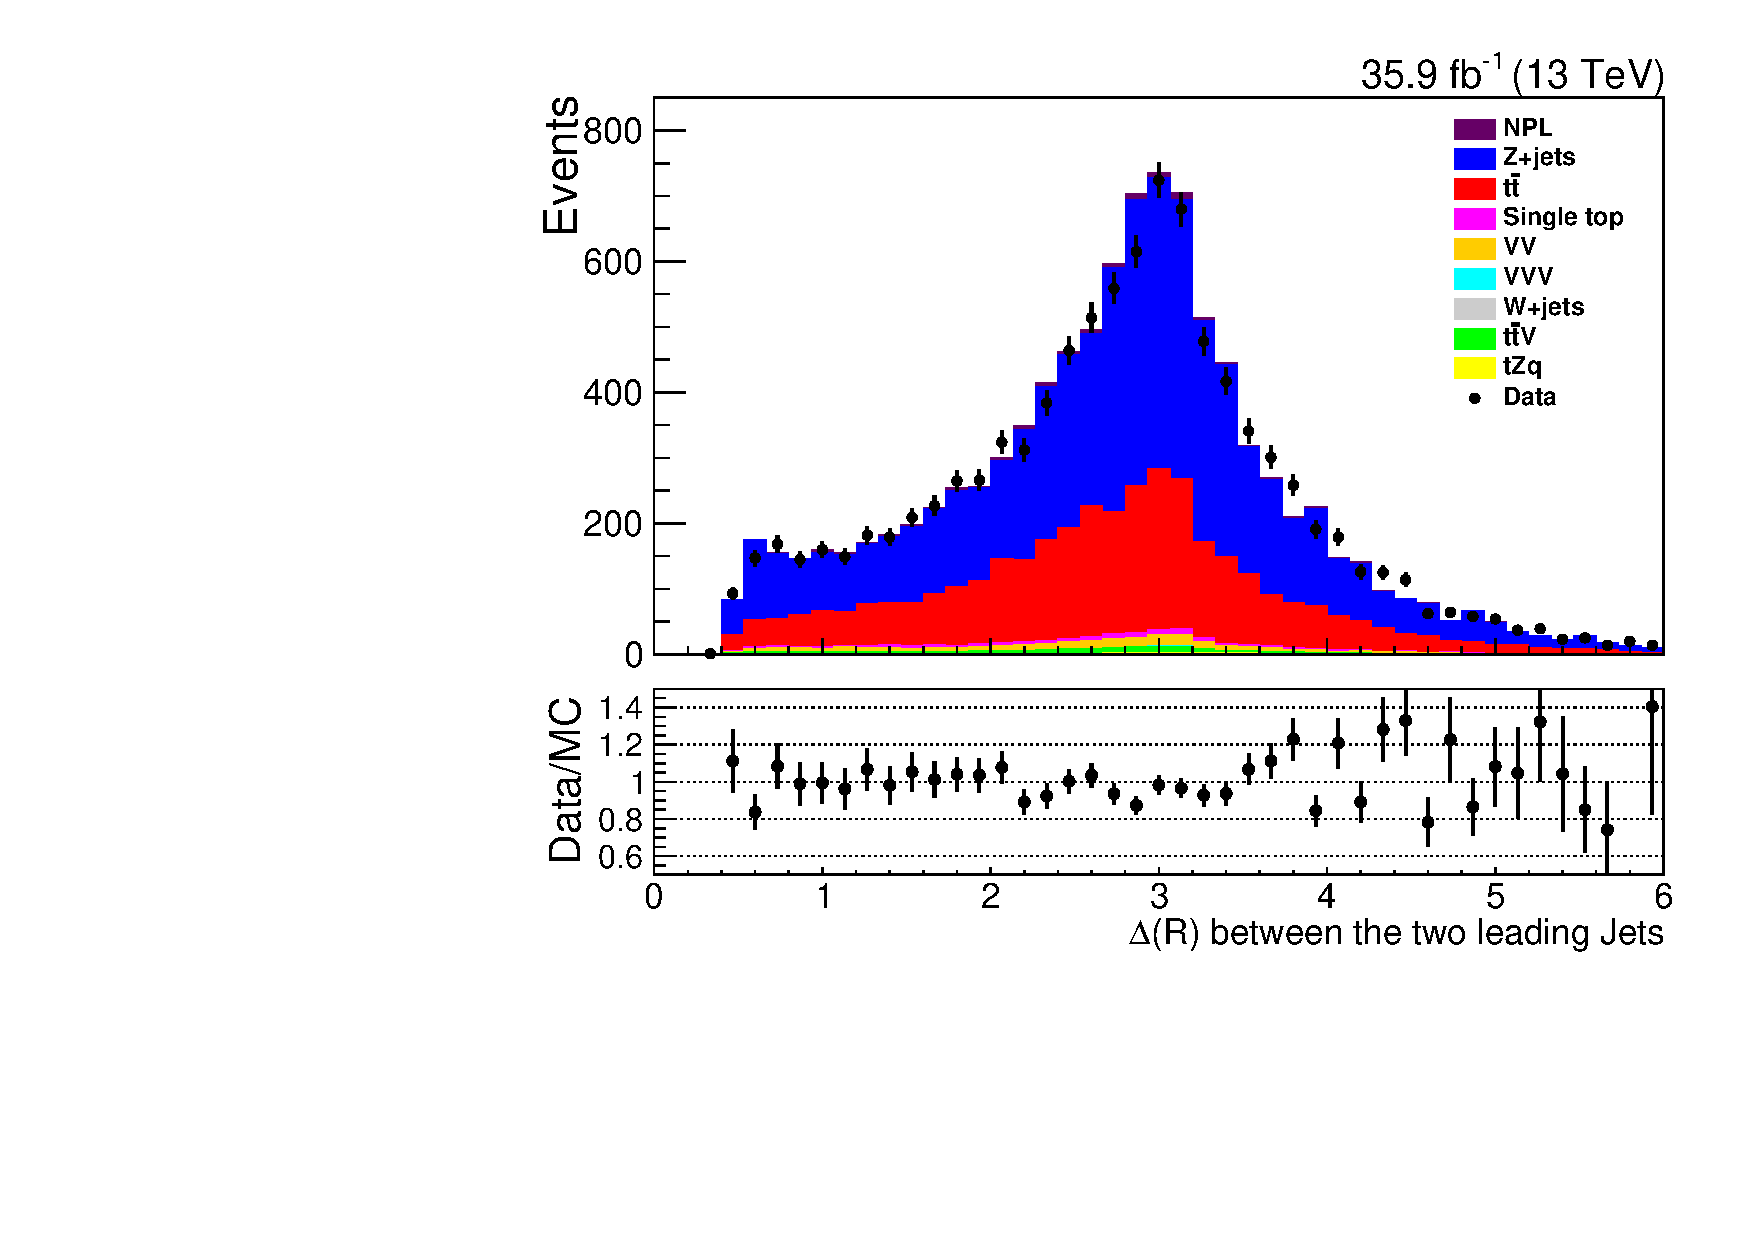
\includegraphics[width=0.47\textwidth]{figs/background-estimation/plots/unblinded/prompt_mumu_ttbarInc/jjDelR_NPL_mumu_wMass_mumu.pdf}
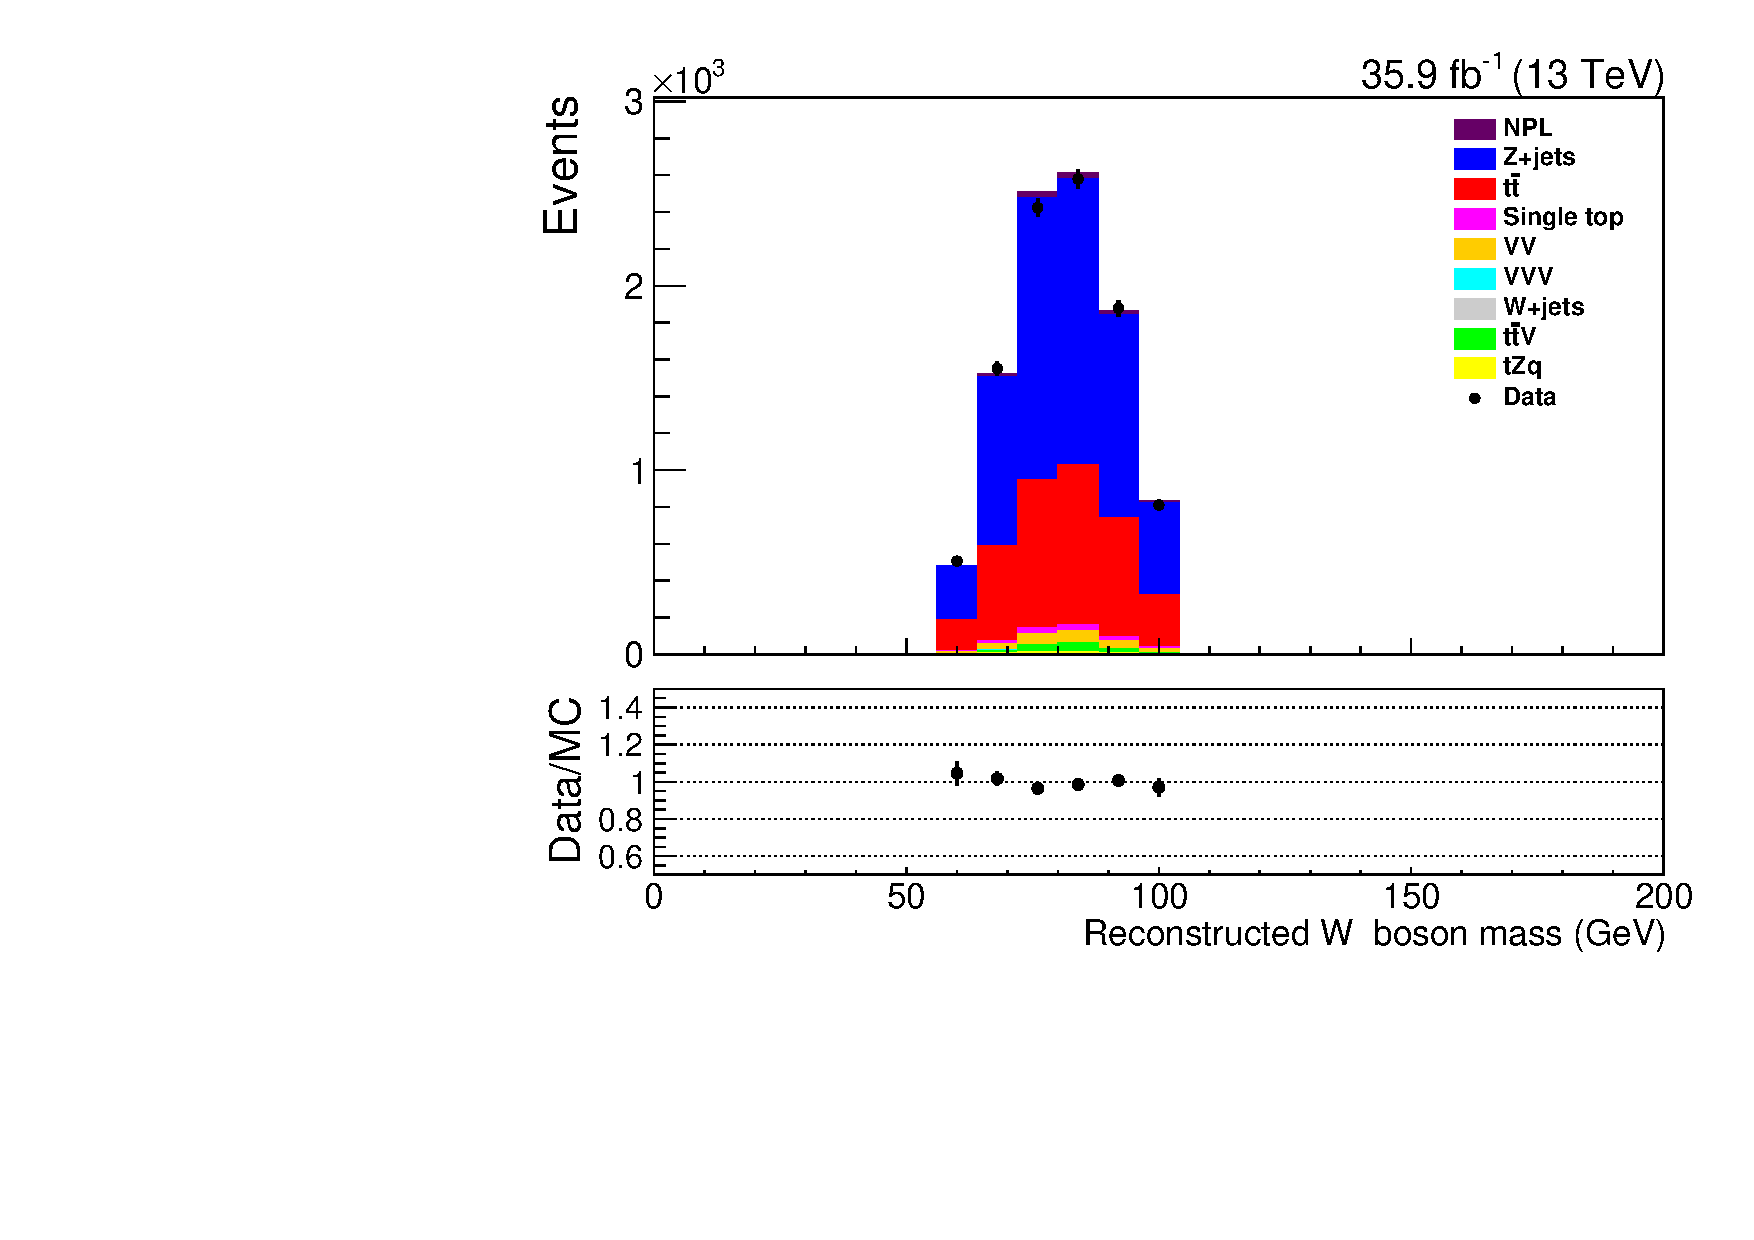
\includegraphics[width=0.47\textwidth]{figs/background-estimation/plots/unblinded/prompt_mumu_ttbarInc/wPairMass_NPL_mumu_wMass_mumu.pdf}
\caption{
Leading b-tagged jet CSVv2 discriminant, leading jet \pT, $\Delta R$ between the leading jets, and reconstructed W boson mass distributions for the $\mu\mu$ channel comparing the agreement between data and simulation for the variables used as input variables in the BDT training.}
\label{fig:inputFeaturesDataSimAgreement2}
\end{figure}

\begin{figure}[h]
\centering
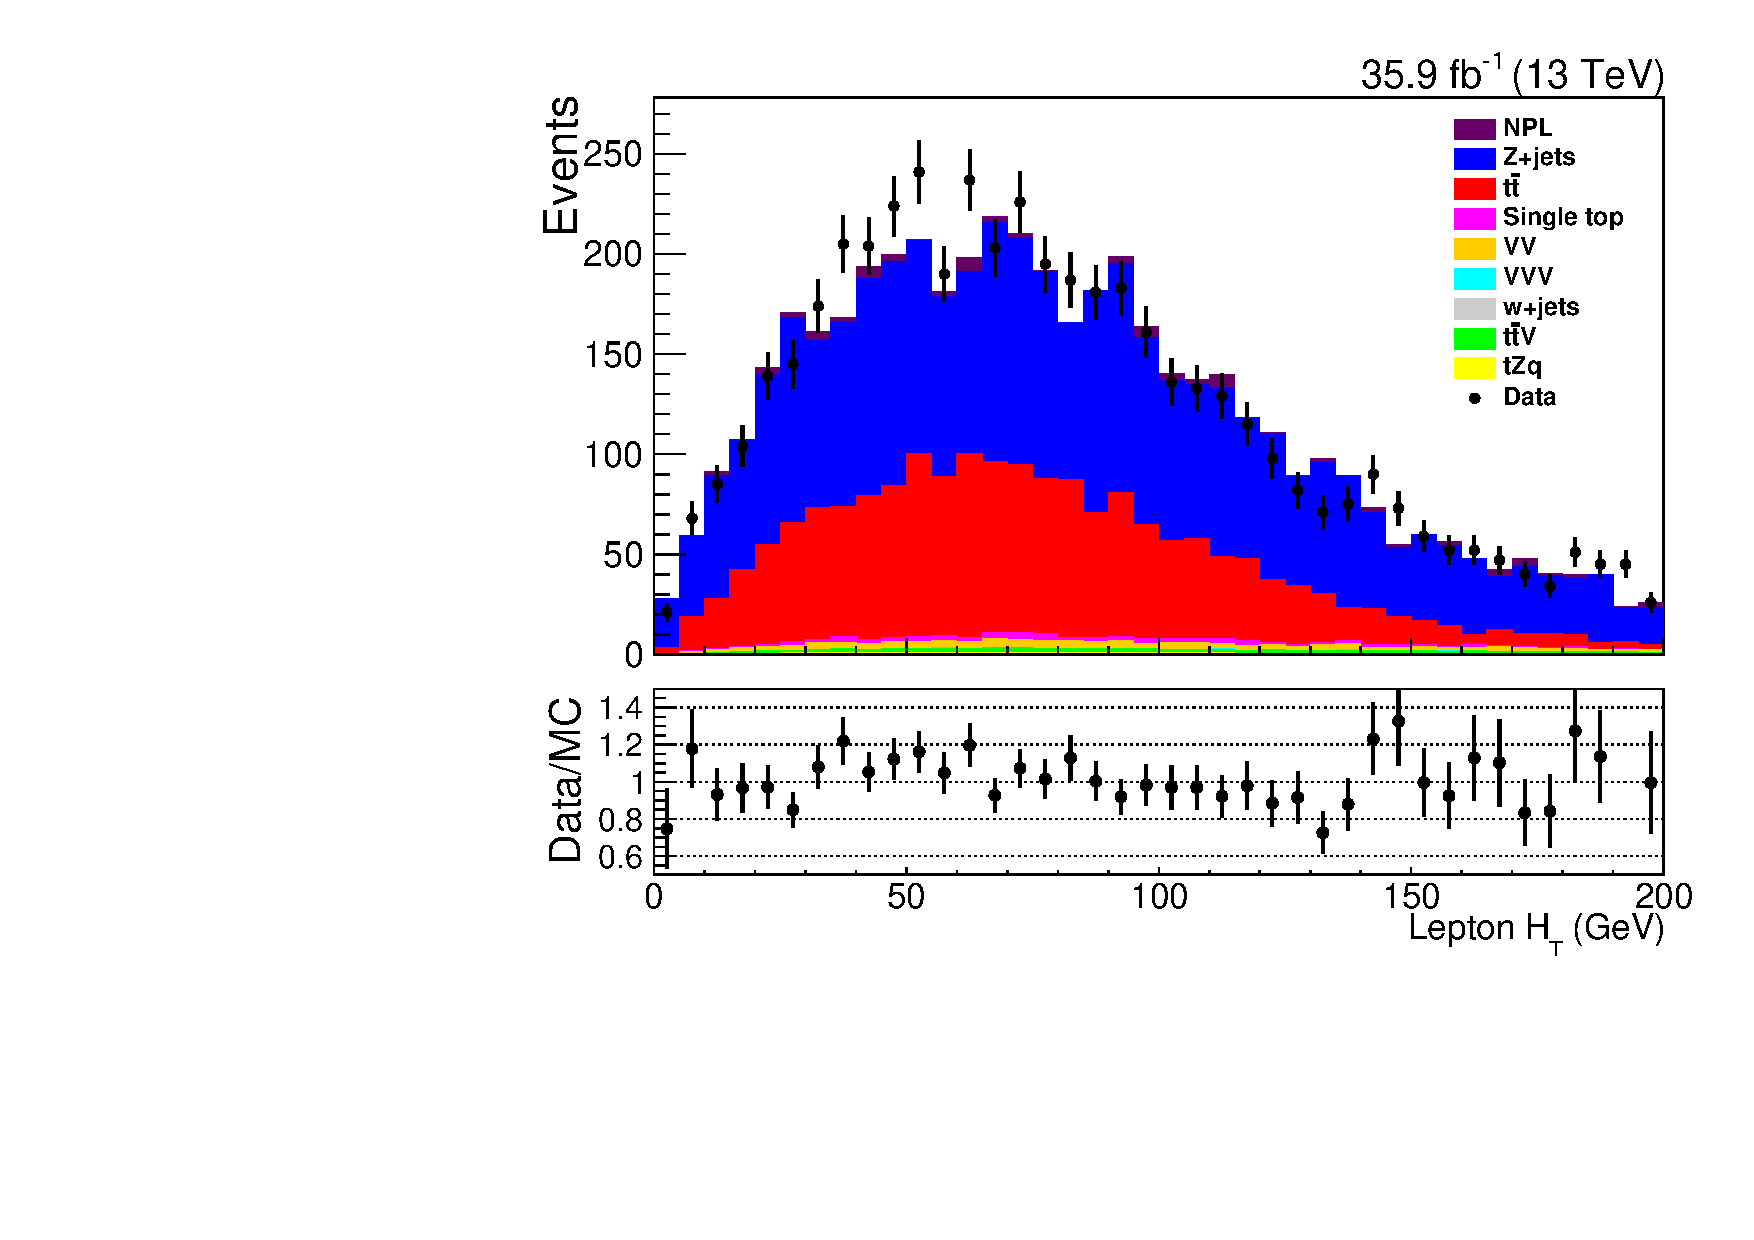
\includegraphics[width=0.47\textwidth]{figs/background-estimation/plots/unblinded/prompt_ee_ttbarInc/lepHt_NPL_ee_wMass_ee.pdf}
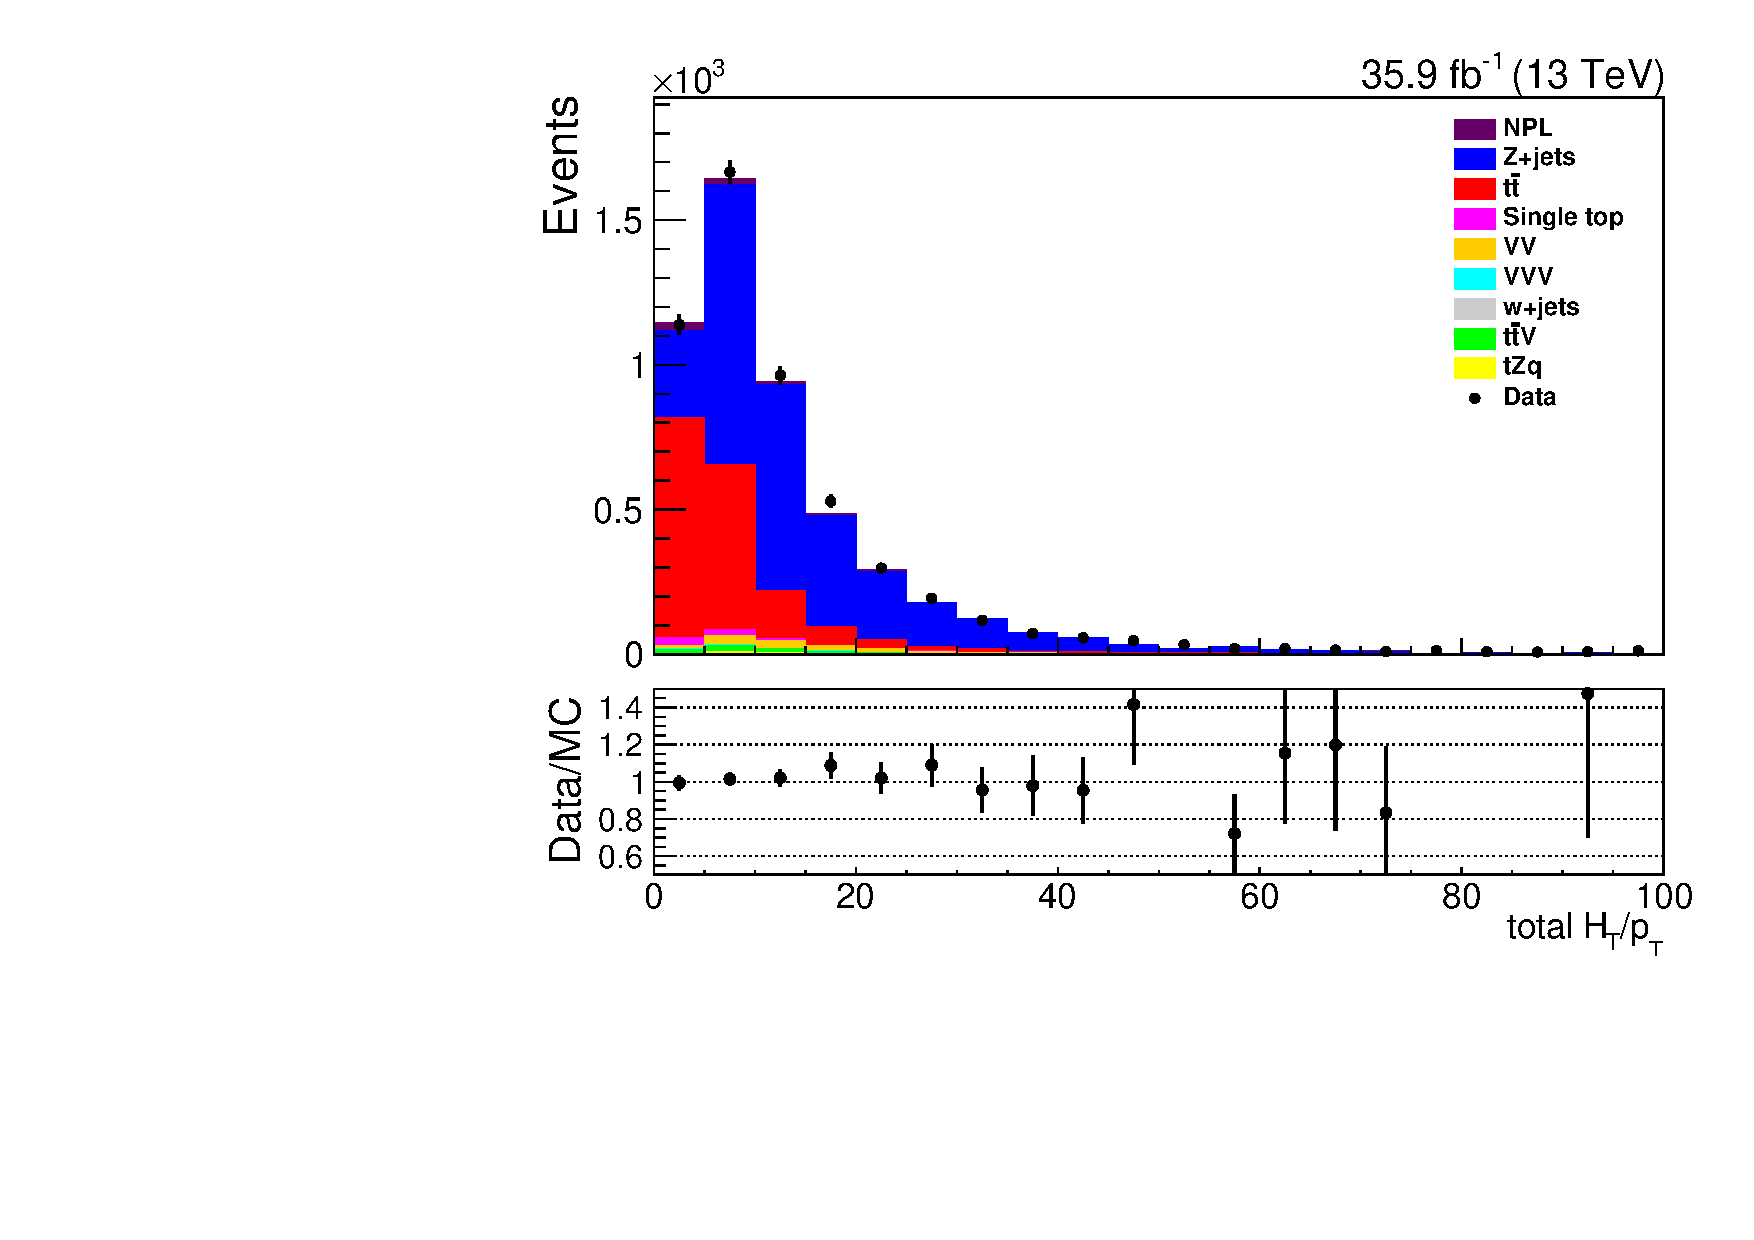
\includegraphics[width=0.47\textwidth]{figs/background-estimation/plots/unblinded/prompt_ee_ttbarInc/totHtOverPt_NPL_ee_wMass_ee.pdf}
\\
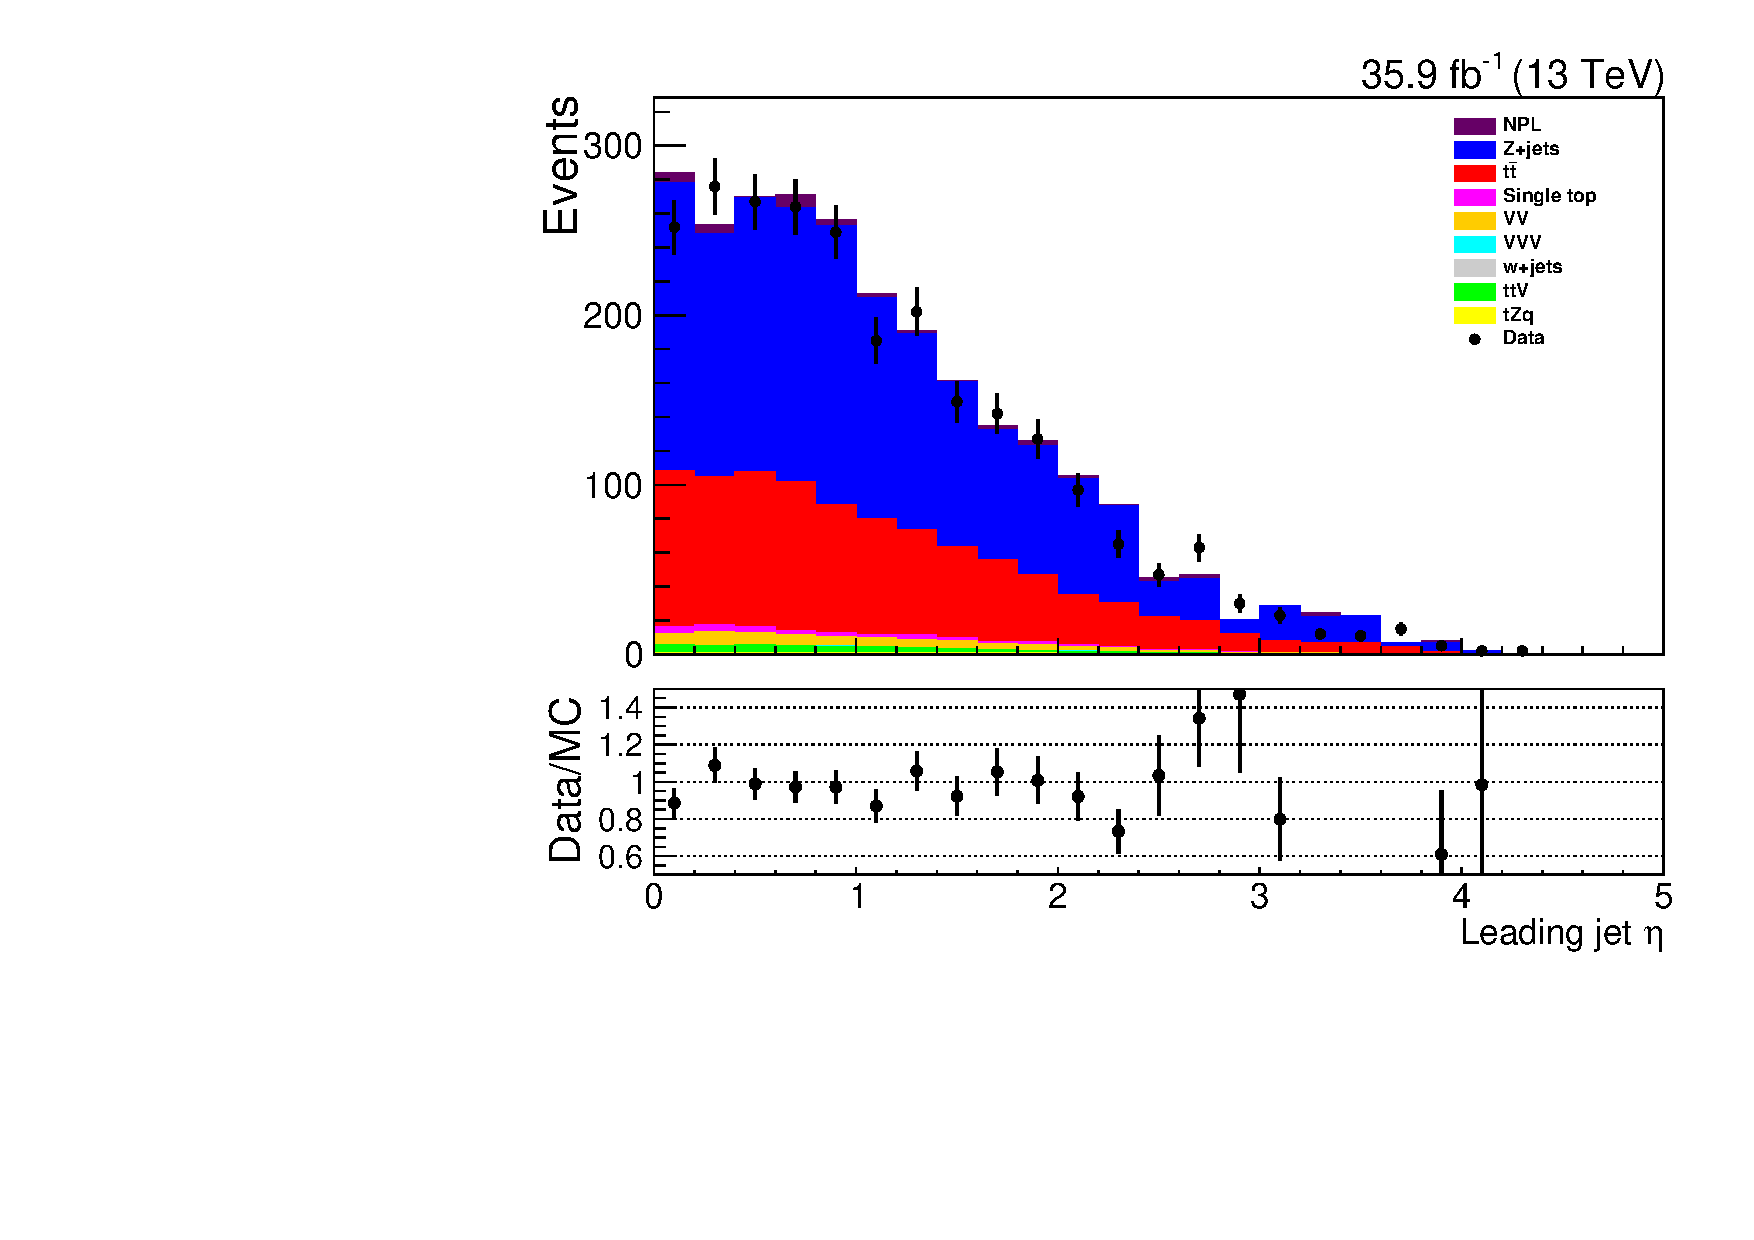
\includegraphics[width=0.47\textwidth]{figs/background-estimation/plots/unblinded/prompt_ee_ttbarInc/leadingJetEta_NPL_ee_wMass_ee.pdf}
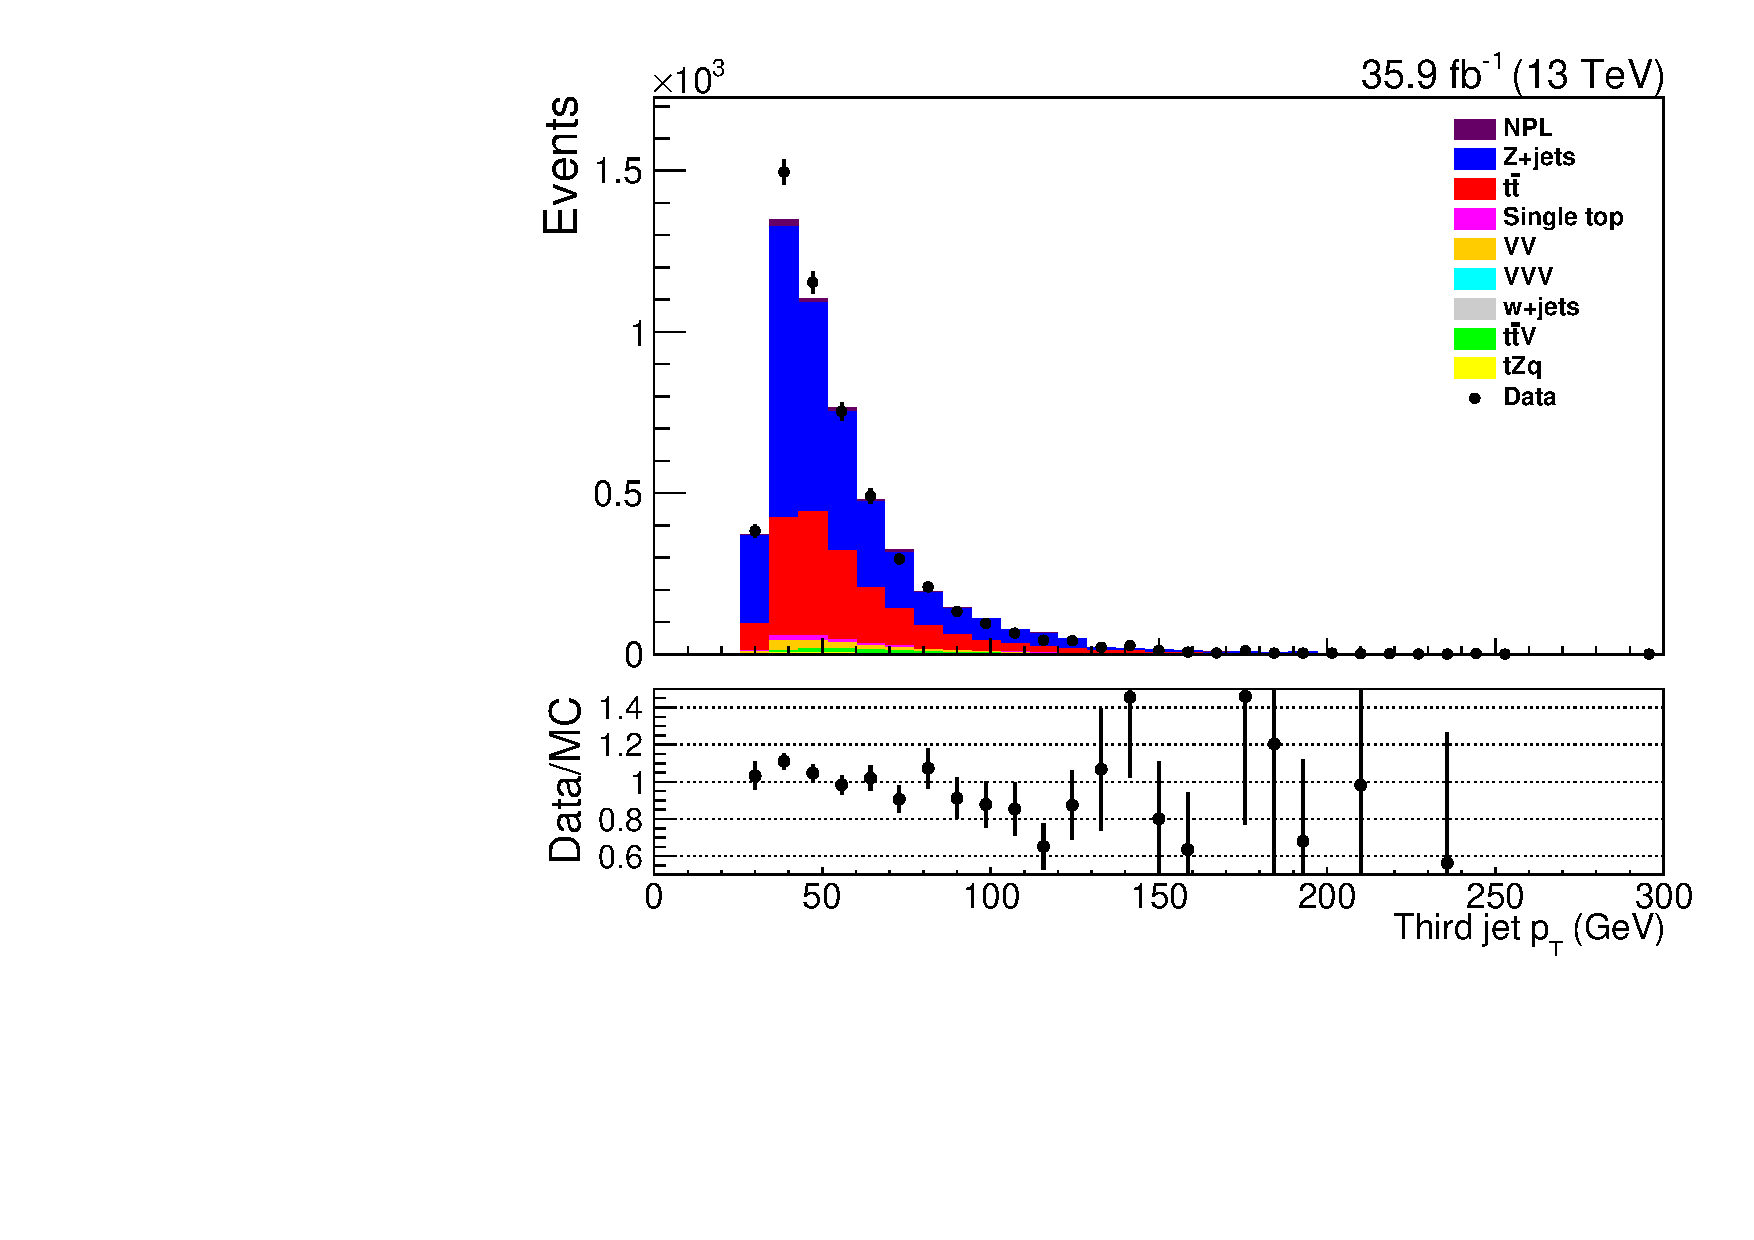
\includegraphics[width=0.47\textwidth]{figs/background-estimation/plots/unblinded/prompt_ee_ttbarInc/thirdJetPt_NPL_ee_wMass_ee.pdf}
\caption{
Lepton ${\ensuremath{H_{\mathrm{T}}}}$, total ${\ensuremath{H_{\mathrm{T}}}}$ divided by total \pt, leading jet $\eta$ and third jet \pT distributions for the $ee$ channel comparing the agreement between data and simulation for the variables used as input variables in the BDT training.}
\label{fig:inputFeaturesDataSimAgreement3}
\end{figure}

\begin{figure}[h]
\centering
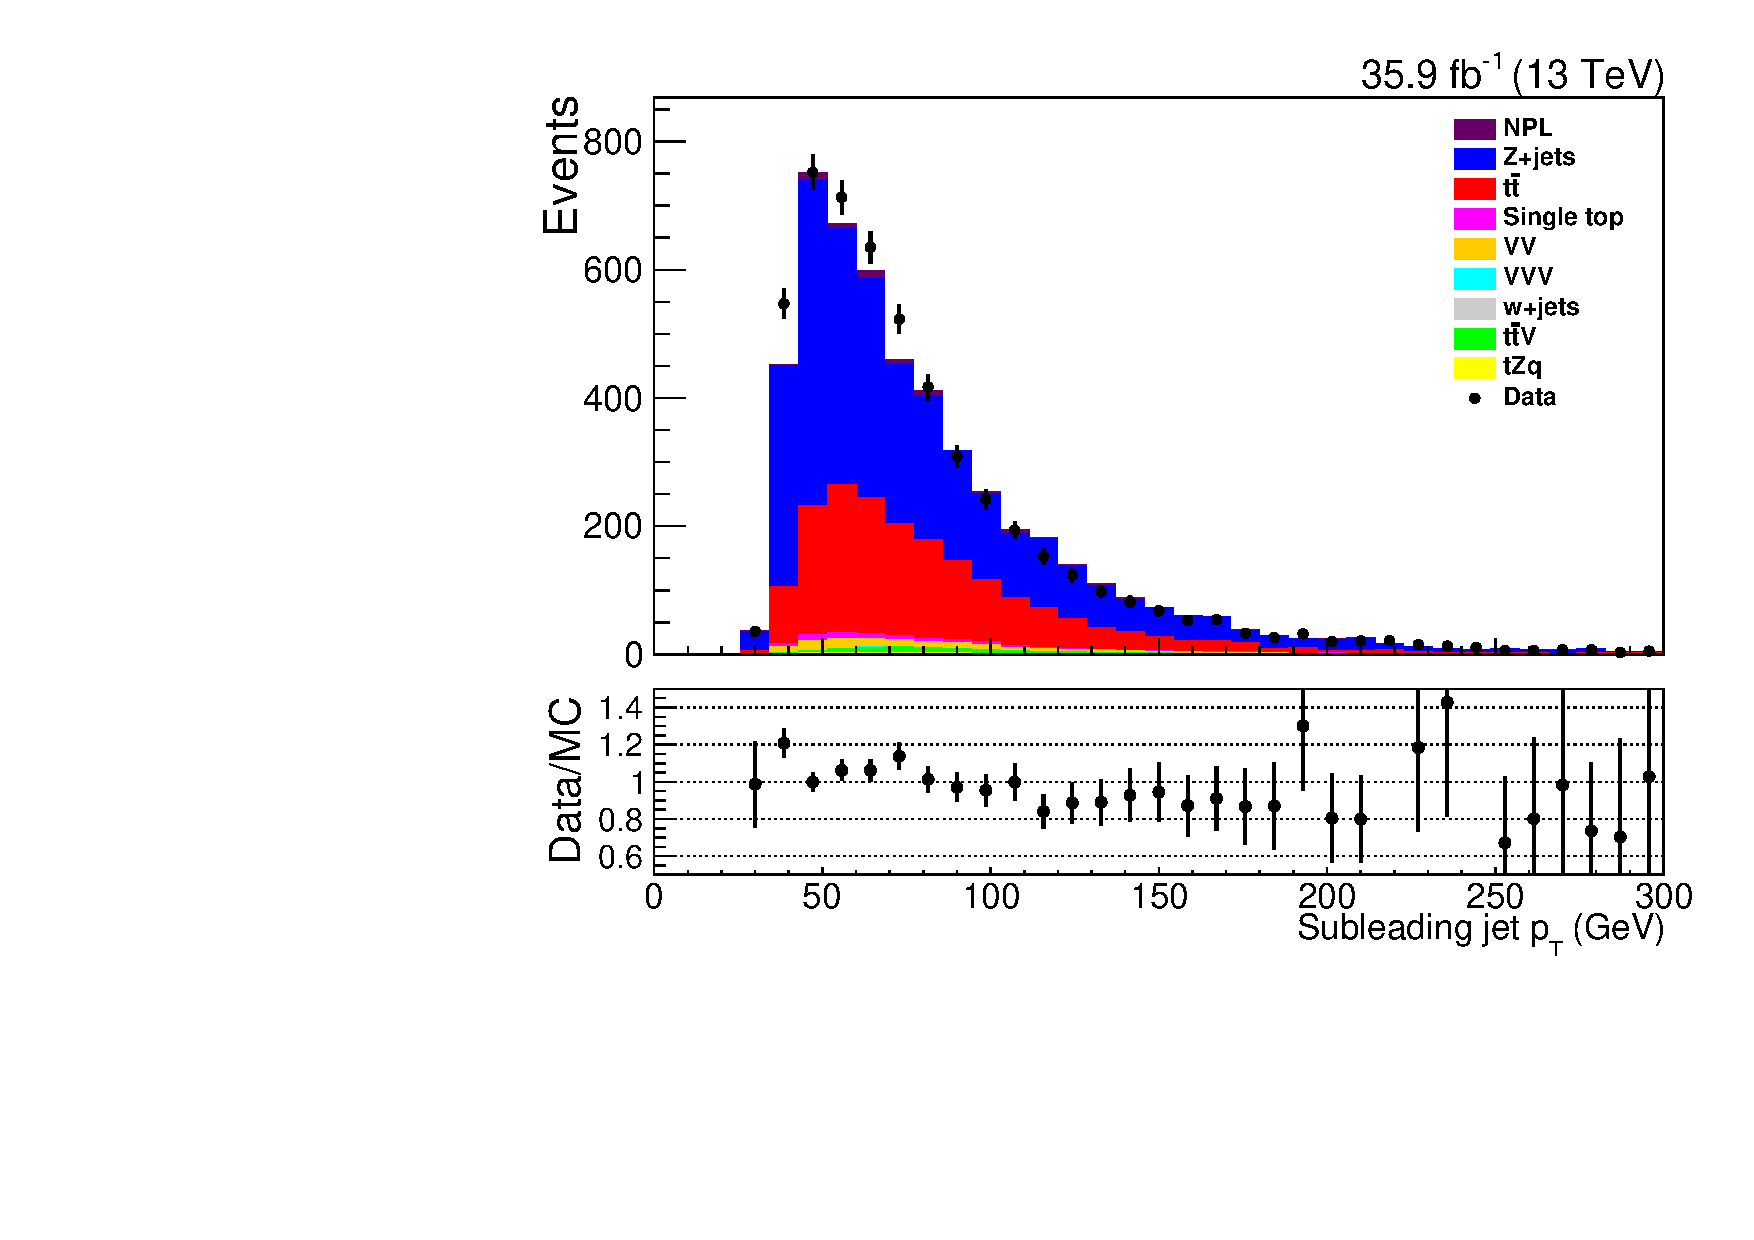
\includegraphics[width=0.47\textwidth]{figs/background-estimation/plots/unblinded/prompt_ee_ttbarInc/secondJetPt_NPL_ee_wMass_ee.pdf}
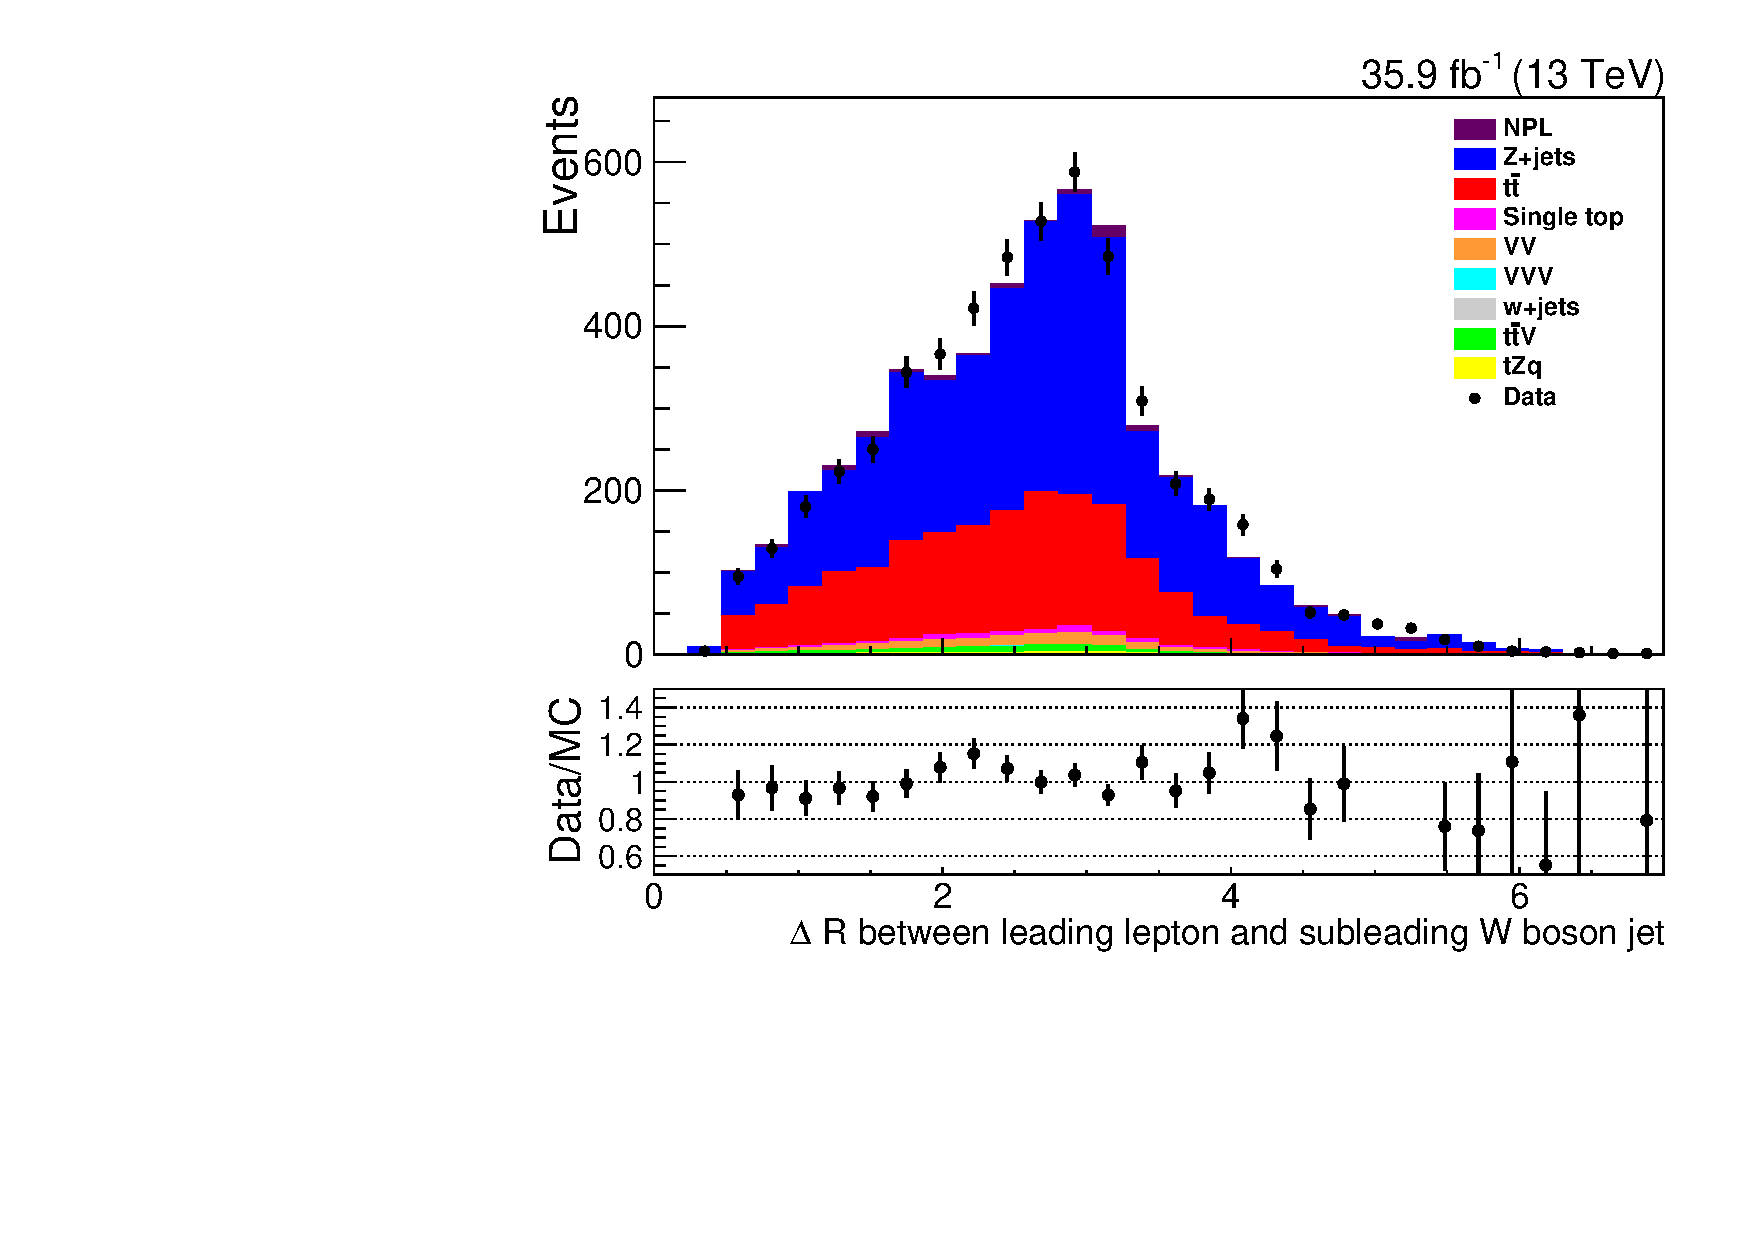
\includegraphics[width=0.47\textwidth]{figs/background-estimation/plots/unblinded/prompt_ee_ttbarInc/zLep1Quark2DelR_NPL_ee_wMass_ee.pdf}
\\
\includegraphics[width=0.47\textwidth]{figs/background-estimation/plots/unblinded/prompt_ee_ttbarInc/zLep2BjetDelR_NPL_ee_wMass_ee.pdf}
\includegraphics[width=0.47\textwidth]{figs/background-estimation/plots/unblinded/prompt_ee_ttbarInc/fourthJetPt_NPL_ee_wMass_ee.pdf}
\caption{
Second jet \pt, $\Delta R$ between subleading lepton and leading b-tagged jet, $\Delta R$ between subleading lepton and leading b-tagged jet and fourth jet \pT distributions for the $ee$ channel comparing the agreement between data and simulation for the variables used as input variables in the BDT training.}
\label{fig:inputFeaturesDataSimAgreement4}
\end{figure}

\begin{figure}[h]
\centering
\includegraphics[width=0.47\textwidth]{figs/background-estimation/plots/unblinded/prompt_mumu_ttbarInc/zLep1BjetDelR_NPL_mumu_wMass_mumu.pdf}
\includegraphics[width=0.47\textwidth]{figs/background-estimation/plots/unblinded/prompt_mumu_ttbarInc/zPairEta_NPL_mumu_wMass_mumu.pdf}
\\
\includegraphics[width=0.47\textwidth]{figs/background-estimation/plots/unblinded/prompt_mumu_ttbarInc/jetHt_NPL_mumu_wMass_mumu.pdf}
\caption{
$\Delta R$ between leading lepton and leading b-tagged jet, reconstructed Z boson $\eta$, and jet ${\ensuremath{H_{\mathrm{T}}}}$ distributions for the $\mu\mu$ channel comparing the agreement between data and simulation for the variables used as input variables in the BDT training.}
\label{fig:inputFeaturesDataSimAgreement5}
\end{figure}

\clearpage
\newpage
%% HYPERPARAMETERS
\subsubsection*{BDT Hyperparameter Optimisation}
Instead of tuning the of choice hyperparameters for optimal classification performance either by hand or using a time and computationally expensive grid search, a regression model was constructed and evaluated using the \emph{Scikit-Optimize} library~\cite{scikit-optimise}.
This regression model identifies the set of optimal hyperparameters as the minima of a metric used to rank the hyperparameters considered.

Table~\ref{tab:hyperparameters} lists the set of hyperparameters and their values for the $ee$ and $\mu\mu$ channels whose optimal values differ from their default values.
Further descriptions of all of the hyperparameters available are given in~\cite{xgboost}.

\begin{table}[htbp]
\topcaption {The optimal hyperparameters for the $ee$ and $\mu\mu$ channels for XGBoost that were found by the regression model and the maximum and minimum values that they can take.
}
\label{tab:hyperparameters}
  \centering
% This increases column spacing.
%\resizebox{\textwidth}{!}{
% This right-aligns numbers in column, but centers them under column title.
\begin{tabular}{lccccc}
   \hline
   \textbf{Option} & \textbf{$ee$} & \textbf{$\mu\mu$}\\
   \hline
    Number of estimators & 5000 & 3282 \\
    Subsample & 0.5 & 1.0 \\
    Learning rate & $2.82\times10^{-3}$ & $19.56\times10^{-3}$  \\
    Maximum tree depth & 2 & 2\\
    Minimum child weight & 1.496 & $1\times10^{-05}$ \\
    $\gamma$ & $56.2\times10^{-3}$ & 5.404 \\
    $\alpha$ & $1.63\times10^{-3}$ & $2.89$ \\
    $\lambda$ & 0.606 & 1.473 \\
   \hline
 \end{tabular}%}
\end{table}

Figure~\ref{fig:bdtResponse} shows the BDT responses for the $ee$ and $\mu\mu$ channels for both the training and testing samples.
As the response of the BDT classifier for both the training and testing samples are consistent with each other, this implies that negligible overtraining has occurred. 

\begin{figure}[htb]
\centering
\includegraphics[width=0.97\textwidth]{figs/background-estimation/plots/response_ee.pdf}
\\
\includegraphics[width=0.97\textwidth]{figs/background-estimation/plots/response_mumu.pdf}
\caption{
Distributions of the input variables chosen for use with the BDT for the signal and background samples.}
\label{fig:bdtResponse}
\end{figure}

Figures~\ref{fig:inputFeaturesDistributions_ee} and~\ref{fig:inputFeaturesDistributions_mumu} shows the distributions of the selected input variables in the signal and background samples for the $ee$ and $\mu\mu$ channels, respectively.

\begin{figure}[htb]
\centering
\vspace*{-3.25cm}\hspace*{-2.3cm}\includegraphics[width=1.27\textwidth]{figs/background-estimation/plots/vars_ee.pdf}
\vspace*{-1cm}\caption{
Distributions of the input variables chosen for use with the BDT for the signal (red) and background (blue) samples for the $ee$ channel.}
\label{fig:inputFeaturesDistributions_ee}
\end{figure}

\begin{figure}[htb]
\centering
\vspace*{-3.25cm}\hspace*{-2.3cm}\includegraphics[width=1.27\textwidth]{figs/background-estimation/plots/vars_mumu.pdf}
\vspace*{-1cm}\caption{
Distributions of the input variables chosen for use with the BDT for the signal (red) and background (blue) samples for the $\mu\mu$ channel.}
\label{fig:inputFeaturesDistributions_mumu}
\end{figure}

\clearpage
\newpage
\subsubsection*{BDT Evaluation}
Following the optimisation of the BDT input variables and hyperparameters, the BDT is trained.
The resultant output discriminant distributions shown in Figure~\ref{fig:prefitBDT}.
These distributions illustrates that there is both good agreement between simulation and data and that the BDT is effective at separating the majority of the backgrounds from the signal.
These output discriminant distributions are used to extract the signal strength and its statistical significance in the following chapter.

\begin{figure}[h]
\centering
\includegraphics[width=0.78\textwidth]{figs/results/prefit_ee.pdf}
\\
\includegraphics[width=0.78\textwidth]{figs/results/prefit_mumu.pdf}
\caption{
Pre-fit distributions of the BDT discriminant for the $ee$ channel (top) and $\mu\mu$ channel (bottom).}
\label{fig:prefitBDT}
\end{figure}
